\documentclass{article}
\usepackage[utf8]{inputenc}
\usepackage[T1]{fontenc}
\usepackage{lmodern}
\usepackage{microtype}
\usepackage{geometry}
\geometry{margin=1in}
\usepackage{setspace}
\onehalfspacing

\usepackage{amsmath,amssymb,amsthm}  
\usepackage{bm}                    
\usepackage{graphicx}             
\usepackage{caption}
\usepackage{subcaption}             
\usepackage{booktabs}                
\usepackage{hyperref}      
\usepackage{algorithm} 
\usepackage{algpseudocode}
\hypersetup{
    colorlinks=true,
    linkcolor=blue,
    citecolor=blue,
    urlcolor=blue
}
\usepackage{natbib}
\usepackage{xcolor,mathtools}                  
\mathtoolsset{showonlyrefs=true}       
\renewcommand{\aa}[1]{{\color{magenta}#1}}
\newtheorem{theorem}{Theorem}[section]
\newtheorem{lemma}[theorem]{Lemma}
\newtheorem{assumption}[theorem]{Assumption}
\newtheorem{corollary}[theorem]{Corollary}
\newcommand{\eqlnostar}[2]{\begin{align}\label{#1}#2\end{align}}
\newcommand{\eqstar}[1]{\begin{align*}#1\end{align*}}
\newcommand{\eq}[1]{\ifthenelse{\equal{#1}{*}}
  {\eqstar}
  {\eqlnostar{#1}}
 }
 
\title{Forecasting implied volatility surface with generative diffusion models\footnote{Full code available on \url{https://github.com/Austinjinc/rep_volgan/tree/refactor/new-ddpm}}}
\author{
Chen JIN\thanks{Department of Statistical and Actuarial Sciences, University of Western Ontario, London, ON, Canada. Email: cjin94@uwo.ca; aagarw93@uwo.ca} \and Ankush AGARWAL\footnotemark[2]
}

\begin{document}

\maketitle
\begin{abstract}
\noindent We introduce a conditional Denoising Diffusion Probabilistic Model (DDPM) for
generating arbitrage-free implied volatility (IV) surfaces, offering a more stable and accurate
alternative to existing GAN-based approaches. To capture the path-dependent nature of
volatility dynamics, our model is conditioned on a rich set of market variables, including
exponential weighted moving averages (EWMAs) of historical surfaces, returns and squared
returns of underlying asset, and scalar risk indicators like VIX. Empirical results demonstrate our
model significantly outperforms leading GAN-based models in capturing the stylized facts of IV
dynamics. A key challenge is that historical data often contains small arbitrage opportunities in
the earlier dataset for training, which conflicts with the goal of generating arbitrage-free
surfaces. We address this by incorporating a standard arbitrage penalty into the loss function,
but apply it using a novel, parameter-free weighting scheme based on the signal-to-noise ratio
(SNR) that dynamically adjusts the penalty's strength across the diffusion process. We
also show a formal analysis of this trade-off and provide a proof of convergence showing that
the penalty introduces a small, controllable bias that steers the model toward the manifold of
arbitrage-free surfaces while ensuring the generated distribution remains close to the real-world data.

\smallskip

\noindent \textbf{Keywords}: Implied volatility; Generative diffusion models; Volatility surface; Arbitrage; Forecasting.

\end{abstract}

\section{Introduction}

The implied volatility (IV) surface summarizes the market's expectation of future asset price uncertainty, it is central to quantitative finance and risk management. However, modelling and forecasting the IV surface is challenging. A valid surface is not an arbitrary collection of points but must satisfy strict no-arbitrage conditions, such as convexity in strike and non-decreasing behavior in time-to-maturity. These constraints mean that valid IV surfaces form a complex, non-linear, low-dimensional manifold embedded within a high-dimensional Euclidean space. An effective generative model must therefore not only capture the complex stochastic dynamics of the surface but also learn the geometry of this arbitrage-free manifold.

Traditional parametric models such as Heston model \citep{Heston_1993}, often impose rigid structural assumptions that fail to capture the full range of shapes observed in the market. With the availability of more computing resources, recent research has turned to deep generative models to learn the IV surface distribution in a data-driven way. These models are highly capable but can be challenging to train, and may suffer from mode collapse, or can struggle to generate statistically reliable uncertainty estimates. Furthermore, they often require carefully designed loss functions to prevent the generation of financially implausible surfaces with obvious arbitrage.

In this paper, we propose a new framework for this task based on Denoising Diffusion Probabilistic Models (DDPMs). DDPMs, which have demonstrated state-of-the-art performance in high-fidelity image generation, are naturally well-suited for this problem. Their stable training process and ability to learn complex data distributions make them an attractive alternative to generative adversarial networks (GANs). We frame the task of forecasting the one-day-ahead IV surface as a conditional generation problem. We adapt the continuous-time generalization of DDPMs, first proposed by \citet{DBLP:journals/corr/abs-2011-13456}, by selecting a Variance Preserving (VP) SDE, which is a natural choice for modelling bounded, normalized volatility data. Our model, based on a U-Net architecture \citep{pmlr-v37-sohl-dickstein15}, learns to approximate the score function of the data distribution, conditioned on previous market information, including the prior day's IV surface and scalar market drivers.

Our primary contribution is the design and application of a novel conditional diffusion model (DDPM) for forecasting the implied volatility surface. A key innovation of this model is its composite loss function, which combines the standard noise-matching objective with an explicit financial arbitrage penalty. This penalty is dynamically weighted by the Signal-to-Noise Ratio (SNR) of the current diffusion step. This weighting scheme prevents erratic gradients from high-noise samples from destabilizing training, while still strongly enforcing no-arbitrage constraints as the model generates the clean surface.

Our comprehensive empirical study shows this approach is highly effective. Compared to a GAN based benchmark, our model not only achieves a lower overall Mean Absolute Percentage Error (MAPE) but also produces better uncertainty estimates. The 90\% confidence intervals from our model are well-calibrated, with breach rates hovering near the theoretical 10\% target, and it generates qualitatively smoother surfaces free of the shape artifacts seen in the output of the GAN based benchmark.

Recent applications of diffusion models to implied volatility surfaces \citep{Hu_2024_tech}, have demonstrated their potential using synthetic data from models like Heston. These studies leverage clean, abundant Monte Carlo samples from the model to focus on unconditional generation or completion tasks, providing valuable insights into the method's capabilities. We move beyond using Monte Carlo samples from a specific model to a more challenging problem of one-day-ahead conditional forecasting with real market data and conditions, a more natural SNR-weighted arbitrage penalty, which yields stable and financially valid forecasts in real-world settings.

Second, we provide a theoretical convergence guarantee for our proposed penalized loss function. We show that for a sufficiently small penalty weight $\lambda$, the bias introduced by the arbitrage term is bounded, and the effective score-matching error $L^{\text{eff}}$ converges to the base model error $L$ with an added bias term of order $O(\lambda^2)$. This result, which leverages a conditional Girsanov theorem and a local strong convexity assumption, provides a convergence proof for a DDPM trained with an explicit financial constraint. This theoretical backing is further supported by recent work from \citet{Tang_Lin_Yang_2024}, which proves that such conditional models are minimax-optimal for distribution estimation on manifolds.

The remainder of this paper is organized as follows. Section \ref{sec:gen_modelling} introduces the generative modelling framework, discussing the manifold of implied volatility surfaces, the forward perturbation process, and the reverse generative SDE. Section \ref{sec:objectives} provides a formal derivation of the training objective, connecting the theoretical goal via Girsanov's theorem to a practical noise-prediction loss. Section \ref{sec:convergence} presents our main theoretical contribution: a convergence proof for the DDPM trained with our explicit arbitrage penalty. Section \ref{sec:procedure} details the practical implementation of our model, including data pre-processing, the conditional U-Net architecture, and our novel SNR-weighted loss function. Section \ref{sec:performance} provides a comprehensive empirical analysis, comparing our model's forecasting performance against the VolGAN benchmark in terms of qualitative, quantitative, and distributional fidelity. Section \ref{sec:conclusion} sums up the paper in the nutshell.

\section{Generative modelling on the Manifold of Implied Volatility Surfaces}
\label{sec:gen_modelling}

\subsection{The Manifold of Arbitrage-Free Implied Volatility Surfaces}

An implied volatility (IV) surface can be represented as a point in a high-dimensional Euclidean space. For a discrete grid of $N_m$ moneyness points and $N_\tau$ tenors, a single surface is an element $x \in \mathbb{R}^{N_m \times N_\tau}$. However, this ambient space also contains surfaces that are financially unviable. A valid IV surface must satisfy a set of no-arbitrage conditions, primarily ensuring convexity in strike (to prevent butterfly arbitrage) and non-decreasing behavior in time-to-maturity (to prevent calendar spread arbitrage) \citep{Gatheral_Jacquier_2014}. These no-arbitrage conditions are given below.

\begin{itemize}
    \item \textbf{No Butterfly Arbitrage (Convexity in Strike):} The price of a butterfly spread must be non-negative. This implies that call prices must be a convex function of the strike price. For call price $c(m, \tau)$ with moneyness $m$ and time to maturity $\tau$, this continuous theoretical condition is:
    $$
    \frac{\partial^2 c(m, \tau)}{\partial m^2} \ge 0.
    $$
    For a discrete grid of moneyness and time-to-maturity $(m_i, \tau_j)$, this is implemented using a finite-difference approximation to check for convexity:
    \begin{equation} \label{eq:no_butterfly}
        \frac{c(m_{i+1}, \tau_j) - c(m_i, \tau_j)}{m_{i+1} - m_i} \ge \frac{c(m_i, \tau_j) - c(m_{i-1}, \tau_j)}{m_i - m_{i-1}} \quad \forall i, j.
    \end{equation}

    \item \textbf{No Calendar Spread Arbitrage (Non-decreasing in Tenor):} The price of a call option must not decrease as time-to-maturity increases. This ensures that a long-dated option is always at least as valuable as a short-dated one with the same strike. The continuous condition is:
    $$
    \frac{\partial c(m, \tau)}{\partial \tau} \ge 0.
    $$
    On our discrete grid, this translates to the simple condition:
    \begin{equation} \label{eq:no_calendar}
        c(m_i, \tau_j) \le c(m_i, \tau_{j+1}) \quad \forall i, j \text{ (where } \tau_{j+1} > \tau_j\text{)}.
    \end{equation}
\end{itemize}
Clearly, these constraints imply that the set of all valid, arbitrage-free IV surfaces does not fill the ambient space. Instead, they form a lower-dimensional, non-linear manifold, which we denote as $\mathcal{M}$, embedded within the higher-dimensional space $\mathbb{R}^{N_m \times N_\tau}$. Thus, any generative model must learn the complex geometry of the data manifold $\mathcal{M}$ while being able to accurately model the stochastic evolution of surfaces on this manifold. Denoising Diffusion Probabilistic Models (DDPMs) provide a powerful, data-driven framework for solving this challenge. The popularity of their application to model complex data distributions is because the model convergence is supported by a theoretical foundation. This convergence was recently established under mild assumptions in the work of \citep{Nakano_2025}.

\subsection{The Forward Diffusion Process: Perturbation from the Manifold}

The first component of a DDPM is the forward process, a fixed procedure that systematically perturbs a data point $x_0 \in \mathcal{M}$ away from the manifold. This process gradually transforms the highly structured data point into a sample from a simple, known prior distribution, typically a standard Gaussian that covers the entire ambient space. The forward process is defined as a discrete-time Markov chain of length $T$. At each step $t \leq T$, a small amount of Gaussian noise is added to the data from the previous step, $x_{t-1}$, according to a pre-defined variance schedule $\{\beta_t\}_{t=1}^T \in (0, 1)$:
\begin{equation}
    q(x_t | x_{t-1}) = \mathcal{N}(x_t; \sqrt{1 - \beta_t} x_{t-1}, \beta_t \mathbf{I}).
\end{equation}
A key property of this process is that we can sample $x_t$ at any arbitrary timestep $t$ directly from the initial data point $x_0$ in a single step. Letting $\alpha_t = 1 - \beta_t$ and $\bar{\alpha}_t = \prod_{i=1}^t \alpha_i$, the closed-form relationship is given as:
\begin{equation} \label{eq:forward_direct}
    x_t = \sqrt{\bar{\alpha}_t} x_0 + \sqrt{1 - \bar{\alpha}_t} \boldsymbol{\epsilon}, \quad \text{where} \quad \boldsymbol{\epsilon} \sim \mathcal{N}(0, \mathbf{I}).
\end{equation}
This property is crucial for an efficient training procedure as it allows for random sampling of timesteps without iterating through the entire chain. As $t \to T$, the distribution of $x_T$ converges to a standard normal distribution since $\bar{\alpha}_t \to 0$. This effectively erases all information about the original manifold structure.

\begin{figure}[h!]
\centering
\includegraphics[width=0.9\linewidth]{fig/diffusion_process_grid.png}
\caption{Diffusion process of the implied volatility.}
\label{fig:diff_process}
\end{figure}

\subsubsection{Terminal Distribution and Approximation Error}
A key step in the DDPM framework is the assumption that the terminal distribution of the forward process $p(x_T)$ can be perfectly replaced by a standard isotropic Gaussian, $p_{\text{prior}}(x_T) = \mathcal{N}(0, \mathbf{I})$. Here, we quantify the error introduced by this approximation. For a fixed initial data point $x_0$, the true distribution at the final step $T$ is $P_1 = p(x_T|x_0) = \mathcal{N}(\sqrt{\bar{\alpha}_T}x_0, (1 - \bar{\alpha}_T)\mathbf{I})$. We compare this to the prior distribution $P_2 = \mathcal{N}(\mathbf{0}, \mathbf{I})$ using the Kullback-Leibler (KL) divergence. The KL divergence between two multivariate Gaussian distributions is given by:
\[
D_{KL}(P_1 \| P_2) = \frac{1}{2} \left( \log \frac{\det \boldsymbol{\Sigma}_2}{\det \boldsymbol{\Sigma}_1} - d + \text{tr}(\boldsymbol{\Sigma}_2^{-1}\boldsymbol{\Sigma}_1) + (\boldsymbol{\mu}_2 - \boldsymbol{\mu}_1)^\top \boldsymbol{\Sigma}_2^{-1} (\boldsymbol{\mu}_2 - \boldsymbol{\mu}_1) \right).
\]
Substituting the means and covariances of $P_1$ and $P_2$, the KL divergence for a given $x_0$ is:
\[
D_{KL}(p(x_T|x_0) \| p_{\text{prior}}(x_T)) = \frac{d}{2} \left( -\log(1 - \bar{\alpha}_T) - \bar{\alpha}_T \right) + \frac{\bar{\alpha}_T}{2} \|x_0\|^2.
\]
To find the overall expected error, we average this quantity over the entire data distribution $p_{\text{data}}(x_0)$:
\[
\mathbb{E}_{x_0}[D_{KL}] = \frac{d}{2} \left( -\log(1 - \bar{\alpha}_T) - \bar{\alpha}_T \right) + \frac{\bar{\alpha}_T}{2} \mathbb{E}_{x_0}[\|x_0\|^2].
\]
For a sufficiently long diffusion process, $\bar{\alpha}_T$ is very small. Using the Taylor expansion $-\log(1-x) - x \approx x^2/2$ for small $x$, the first term is of order $\mathcal{O}(d\bar{\alpha}_T^2)$. If the data is standardized to have approximately unit variance per dimension, then $\mathbb{E}[\|x_0\|^2] \approx d$, making the second term of order $\mathcal{O}(d\bar{\alpha}_T)$. The linear term dominates, so the expected KL divergence is bounded by $\mathbb{E}_{x_0}[D_{KL}] \approx \mathcal{O}(d\bar{\alpha}_T)$.

Finally, applying Pinsker's inequality, which relates the Total Variation (TV) distance to the KL divergence ($D_{TV} \le \sqrt{\frac{1}{2} D_{KL}}$), gives the final bound on the terminal error:
\[
\text{Error}_{\text{Terminal}} = D_{TV}(p(x_T), p_{\text{prior}}) \le \sqrt{\frac{1}{2} \mathcal{O}(d\bar{\alpha}_T)} = \mathcal{O}(\sqrt{d\bar{\alpha}_T}).
\]
This shows that for a well-designed variance schedule where $\bar{\alpha}_T \to 0$, the approximation error is controllable and can be made arbitrarily small, thus justifying the use of a standard normal prior in the reverse process.

\subsection{Continuous-Time Generalization via SDEs}

As shown by \citet{DBLP:journals/corr/abs-2011-13456}, this discrete-step process can be generalized into a more powerful continuous-time framework. When the number of steps $T \to \infty$, the discrete chain converges to the solution of a specific Stochastic Differential Equation (SDE). This SDE describes the continuous evolution of the data distribution over time $t \in [0, T]$:
\eqlnostar{eq:forward process}{
d\mathbf{x} = \mathbf{f}(\mathbf{x}, t)dt + g(t)d\mathbf{w}.}
Here, $\mathbf{f}(\mathbf{x}, t)$ is the \textit{drift coefficient} and $g(t)$ is the \textit{diffusion coefficient}. The specific forms of these functions are chosen by the modeler to define the forward process. The two most prominent formulations are:

\begin{itemize}
    \item \textbf{Variance Preserving (VP) SDE:} This is the direct continuous-time generalization of the DDPM formulation. The drift and diffusion coefficients are defined by a continuous noise schedule $\beta(t) \in (0, 1)$ as:
    $$
    \mathbf{f}(\mathbf{x}, t) = -\frac{1}{2}\beta(t)\mathbf{x} \quad \text{and} \quad g(t) = \sqrt{\beta(t)}.
    $$
    This results in the SDE:
    \eqlnostar{eq:vp sde}{
    d\mathbf{x} = -\frac{1}{2}\beta(t)\mathbf{x} dt + \sqrt{\beta(t)}d\mathbf{w}.}
    This SDE is designed to keep the variance of the perturbed data bounded.

    \item \textbf{Variance Exploding (VE) SDE:} This formulation generalizes score-matching models (NCSN). It uses a zero drift and a diffusion coefficient defined by an increasing noise scale $\sigma(t)$:
    $$
    \mathbf{f}(\mathbf{x}, t) = \mathbf{0} \quad \text{and} \quad g(t) = \sqrt{\frac{d[\sigma^2(t)]}{dt}}.
    $$
    This results in the SDE:
    \eqlnostar{eq:ve sde}{
    d\mathbf{x} = \sqrt{\frac{d[\sigma^2(t)]}{dt}}d\mathbf{w},
    }
    where the variance of $\mathbf{x}_t$ grows over time.
\end{itemize}
Here, $\sigma(t)$ is an increasing function of time that defines the noise scale. This formulation is effective for data where the scale is not necessarily normalized as it focuses on matching the score at different noise levels, regardless of the data's original variance.

The primary difference between these SDEs lies in how they perturb the data and manage the variance of the resulting distribution.
\begin{itemize}
    \item VP-SDE \eqref{eq:vp sde} perturbs data such that the variance stays roughly constant. It is analogous to corrupting a clean signal with noise while rescaling it to maintain its power.
    \item VE-SDE \eqref{eq:ve sde} only adds noise, causing the variance to increase over time. This is analogous to corrupting a clean signal with noise of a progressively larger magnitude, which eventually dominates the signal.
\end{itemize}
Despite these differences in the forward process, the insight from \citet{DBLP:journals/corr/abs-2011-13456} is that all of these forward SDEs have a corresponding reverse SDE that depends on the score of the perturbed data distribution, $\nabla_{\mathbf{x}} \log p_t(\mathbf{x})$. We will introduce the reverse SDE details in Section \ref{subsec: reverse_SDE}. The choice between these SDE formulations is therefore a critical modelling decision, which depends on the characteristics of the application and data.
The VE-SDE is highly effective for data where the absolute scale is less significant, as it corrupts the signal by adding noise of ever-increasing magnitude. In contrast, the VP-SDE is specifically designed for data that is well-scaled or normalized to a fixed range. It perturbs the data while ensuring its overall variance remains approximately constant throughout the diffusion process.

We use VP-SDE because normalized volatilities are bounded. This simplifies training compared to VE-SDE. This allows the model to focus entirely on learning the structural features of the smile and skew, leading to a more direct and stable learning objective compared to the other choices.

\subsection{The Reverse Process: Learning the Drift Towards the Manifold}
\label{subsec: reverse_SDE}
The generative component of the model is the reverse process, which learns to reverse the diffusion. Conceptually, it learns a path from a point of pure noise in the ambient space back towards the data manifold $\mathcal{M}$. The model learns the score function toward the high-density regions corresponding to valid IV surfaces.

The feasibility of reversing this process \citet{Anderson_1982} demonstrates that a forward-time SDE has a corresponding reverse-time SDE that describes the same diffusion process but evolving backwards in time. For the forward process described previously in \eqref{eq:forward process}, its reverse is given by:
$$ d\mathbf{x} = [\mathbf{f}(\mathbf{x}, t) - g(t)^2 \nabla_{\mathbf{x}}\log p_t(\mathbf{x})]dt + g(t)d\bar{\mathbf{w}}.$$
Here, $d\bar{\mathbf{w}}$ is a standard Wiener process when time flows backwards from $T$ to $0$. The drift term consists of the original forward drift $\mathbf{f}(\mathbf{x}, t)$ corrected by a crucial term: the gradient of the log-density of the perturbed data, $\nabla_{\mathbf{x}}\log p_t(\mathbf{x})$. This gradient is known as the score function.

While the reverse SDE provides a theoretical path for generation, it is not immediately computable because it depends on the score of the marginal distributions $\{p_t(\mathbf{x})\}_{t \in [0,T]}$, which are unknown. The core task of the generative model is therefore to learn a time-dependent neural network, $\mathbf{s}_\theta(\mathbf{x}, t)$, to approximate the true score function $s^*$. For the VP-SDE used in this work, the score function is directly related to the noise component $\boldsymbol{\epsilon}$ from the forward process. This insight allows us to re-parameterize our score model $\mathbf{s}_\theta(\mathbf{x}_t, t)$ in terms of a neural network $\boldsymbol{\epsilon}_\theta(\mathbf{x}_t, t)$ trained to predict the noise from the noisy data. This relationship is given by:
$$
\mathbf{s}_\theta(\mathbf{x}_t, t) = -\frac{\boldsymbol{\epsilon}_\theta(\mathbf{x}_t, t)}{\sqrt{1 - \bar{\alpha}_t}}.
$$
This approach is not only functionally equivalent to learning the score but is often more stable in practice.

As established in the preceding sections, minimizing the KL divergence between the true and model-generated trajectories is equivalent to minimizing a weighted score-matching objective. Through the noise-prediction parameterization shown above, this objective simplifies to the following L2 loss between the true and predicted noise:
\begin{equation}
    \mathcal{L}_{simple} = \mathbb{E}_{t, \mathbf{x}_0, \boldsymbol{\epsilon}} \left[ ||\boldsymbol{\epsilon} - \boldsymbol{\epsilon}_\theta(\mathbf{x}_t, t)||^2 \right].
\end{equation}
Minimizing this objective effectively trains the score-approximating network. Once trained, the learned function $\boldsymbol{\epsilon}_\theta$ is used to estimate the score and numerically solve the reverse SDE, generating implied volatility surfaces from pure noise.

\section{Derivation of the Training Objective}
\label{sec:objectives}
The objective of the generative model is to learn the reverse process that transforms a simple prior distribution into the complex data distribution. This is formally achieved by minimizing the Kullback-Leibler (KL) divergence between the path distribution generated by our model, $P_\theta$, and the true reverse process distribution, $Q$.

\subsection{Theoretical Objective via Girsanov's Theorem}
The KL divergence provides a natural measure of similarity between the two process distributions. For processes defined by Stochastic Differential Equations (SDEs), Girsanov's theorem offers a direct way to compute this divergence.

Let's consider the continuous-time reverse SDEs for the true process (driven by the true score $s^*$) and our parameterized model (driven by the learned score $s_\theta$):
\begin{align*}
    \text{True Process (Q):} \quad d\mathbf{x} &= \left[\mathbf{f}(\mathbf{x}, t) - g(t)^2 s^*(\mathbf{x}, t)\right]dt + g(t)d\bar{\mathbf{w}} \\
    \text{Model Process ($P_\theta$):} \quad d\mathbf{x} &= \left[\mathbf{f}(\mathbf{x}, t) - g(t)^2 s_\theta(\mathbf{x}, t)\right]dt + g(t)d\bar{\mathbf{w}}.
\end{align*}
The two processes share the same diffusion term $g(t)d\bar{\mathbf{w}}$ and differ only in their drift. The difference in drift is given by:
\[
\text{Drift Difference} = \left[\mathbf{f}(\mathbf{x}, t) - g(t)^2 s_\theta(\mathbf{x}, t)\right] - \left[\mathbf{f}(\mathbf{x}, t) - g(t)^2 s^*(\mathbf{x}, t)\right] = g(t)^2 (s^* - s_\theta).
\]
Girsanov's theorem states that the KL divergence between the path measures $P_\theta$ and $Q$ is half the expected squared norm of the drift difference, scaled by the diffusion coefficient and integrated over time:
\begin{align}
    D_{KL}(P_\theta \| Q) &= \frac{1}{2} \mathbb{E} \left[ \int_0^T \left\| \frac{g(t)^2 (s^*(\mathbf{x}_t, t) - s_\theta(\mathbf{x}_t, t))}{g(t)} \right\|^2 dt \right] \nonumber \\
    &= \frac{1}{2} \mathbb{E} \left[ \int_0^T g(t)^2 \|s^*(\mathbf{x}_t, t) - s_\theta(\mathbf{x}_t, t)\|^2 dt \right].
\end{align}

This fundamental result \citep{Revuz_Yor_1999} establishes that minimizing the KL divergence between the process distributions is equivalent to a continuous-time, weighted score-matching objective. This provides the core theoretical justification for the entire training procedure.

\subsection{Practical Implementation via Noise Prediction}
While Girsanov's theorem provides the theoretically sound objective of matching the score, its practical implementation is enabled by a specific parameterization of the score model. As established in the original DDPM framework \citep{Ho_Jain_Abbeel_2020}, the true score of the perturbed data distribution is directly related to the noise $\boldsymbol{\epsilon}$ added during the forward process:
$$
s^*(\mathbf{x}_t, t) = \nabla_{\mathbf{x}_t} \log p_t(\mathbf{x}_t | \mathbf{x}_0) = -\frac{\boldsymbol{\epsilon}}{\sqrt{1 - \bar{\alpha}_t}}.
$$
We can therefore parameterize our model's score $s_\theta$ to have the same functional form, using a neural network $\boldsymbol{\epsilon}_\theta(\mathbf{x}_t, t)$ to predict the noise $\boldsymbol{\epsilon}$ from the noisy data $\mathbf{x}_t$:
$$
s_\theta(\mathbf{x}_t, t) = -\frac{\boldsymbol{\epsilon}_\theta(\mathbf{x}_t, t)}{\sqrt{1 - \bar{\alpha}_t}}.
$$
Substituting these two expressions into our score-matching objective from Girsanov's theorem connects the theoretical goal to a practical noise-prediction task. The continuous integral becomes a sum over discrete timesteps, and the objective becomes minimizing:
\begin{align}
L(\theta) &\propto \sum_{t=1}^T \lambda(t) \mathbb{E}_{\mathbf{x}_0, \boldsymbol{\epsilon}} \left[ \left\| -\frac{\boldsymbol{\epsilon}}{\sqrt{1 - \bar{\alpha}_t}} - \left(-\frac{\boldsymbol{\epsilon}_\theta(\mathbf{x}_t, t)}{\sqrt{1 - \bar{\alpha}_t}}\right) \right\|^2 \right] \nonumber \\
&= \sum_{t=1}^T \lambda(t) \mathbb{E}_{\mathbf{x}_0, \boldsymbol{\epsilon}} \left[ \frac{1}{1 - \bar{\alpha}_t} \left\| \boldsymbol{\epsilon} - \boldsymbol{\epsilon}_\theta(\mathbf{x}_t, t) \right\|^2 \right],
\end{align}
where $\lambda(t)$ is a positive weighting function derived from the SDE coefficients (e.g., related to $g(t)^2$). As shown by \citet{Ho_Jain_Abbeel_2020}, empirically dropping this complex weighting term and using a uniform weight leads to a more stable training process and excellent results. This yields the final simplified loss function:
\begin{equation}
    L_{\text{simple}}(\theta) = \mathbb{E}_{t, \mathbf{x}_0, \boldsymbol{\epsilon}} \left[ || \boldsymbol{\epsilon} - \boldsymbol{\epsilon}_\theta(\sqrt{\bar{\alpha}_t} \mathbf{x}_0 + \sqrt{1 - \bar{\alpha}_t} \boldsymbol{\epsilon}, t) ||^2 \right].
\end{equation}

\subsection{Adapting for Conditional Dynamics}
The unconditional framework derived above is adapted for forecasting via conditional generation. The model is directly conditioned on covariates (prior-day IV surface and scalar drivers) without an external classifier. This aligns with the conditional forward-backward diffusion models analyzed by \citet{Tang_Lin_Yang_2024}, who proved minimax-optimal convergence rates for such estimators under the total variation metric—extending to manifold adaptation where error bounds depend only on intrinsic data dimensions.

Practically, this is achieved by augmenting the noise prediction network, $\boldsymbol{\epsilon}_\theta$, to accept the conditioning vector $\mathbf{c}$ as an additional input: $\boldsymbol{\epsilon}_\theta(\mathbf{x}_t, t, \mathbf{c})$. The loss function retains its simple mean-squared error form, with the expectation now also taken over the distribution of conditions:
$$
L_{\text{conditional}}(\theta) = \mathbb{E}_{t, \mathbf{x}_0, \boldsymbol{\epsilon}, \mathbf{c}} \left[ || \boldsymbol{\epsilon} - \boldsymbol{\epsilon}_\theta(\mathbf{x}_t, t, \mathbf{c}) ||^2 \right].
$$
In our model, the conditioning vector $\mathbf{c}$ includes the previous day's surfaces and scalar drivers derived from parametric models, which enables the model to capture stochastic evolutions on the arbitrage-free manifold. We will elaborate on the condition details later in Section \ref{subsec:Architectures_Conditions}.



\section{Convergence of DDPM with Arbitrage Penalty}
\label{sec:convergence}
The proof proceeds in three main parts:
\begin{enumerate}
    \item We first analyze the bias introduced by the arbitrage penalty term in the loss function, using a local strong convexity assumption.
    \item We then use a conditional version of the Girsanov theorem to relate the error in the learned score function to the KL Divergence between the generated and true data paths.
    \item Finally, we combine these results with standard DDPM error terms (discretization and terminal errors) to derive a comprehensive bound on the TV distance, leveraging Pinsker's inequality \citep{chen2025diffusionfactormodelsgenerating, Tsybakov_2009}.
\end{enumerate}


\subsection{Notation}
\begin{itemize}
    \item Data distribution: $\mu_{\text{data}}(\mathbf{x} \mid \mathbf{c})$, where $\mathbf{x} \in \mathbb{R}^d$ is the vectorized IV surface ($d=81$), and $\mathbf{c}$ is the conditioning information.
    \item Forward process: $\mathbf{x}_t = \sqrt{\bar{\alpha}_t} \mathbf{x}_0 + \sqrt{1 - \bar{\alpha}_t} \epsilon$, for $\epsilon \sim \mathcal{N}(0, I)$ and $t=1, \dots, n$.
    \item Model: A U-Net with parameters $\theta$ that predicts noise $\hat{\epsilon}_\theta(\mathbf{x}_t, t, \mathbf{c})$.
    \item Score Functions: The true score is $s^*(\mathbf{x}_t, t, \mathbf{c}) = \nabla_{\mathbf{x}_t} \log p_t(\mathbf{x}_t \mid \mathbf{c})$. The model's score is $s_\theta$.
    \item Loss Function: $\mathcal{L}(\theta) = \mathcal{L}_{\text{MSE}}(\theta) + \lambda \mathcal{L}_{\text{arb}}(\theta)$, where $\mathcal{L}_{\text{MSE}} = \mathbb{E} [ \| \epsilon - \hat{\epsilon}_\theta \|^2 ]$ and $\mathcal{L}_{\text{arb}}$ is the arbitrage penalty.
\end{itemize}

\subsection{Assumptions}
The following assumptions are required for the proof to hold.

\begin{assumption}[Bounded Data and Scores] \label{ass:bounded_data}
The Implied volatility data and conditioning information are bounded in Euclidean norm by constants $M_\mathbf{x}$ and $M_\mathbf{c}$. The true conditional score $s^*(\mathbf{x}_t, t, \mathbf{c})$ is $K$-Lipschitz with respect to its data input $\mathbf{x}_t$ and exhibits at most linear growth, satisfying:
\[
\|s^*(\mathbf{x}_t, t, \mathbf{c})\| \le K(1 + \|\mathbf{x}_t\|),
\]
for a positive constant $K$.
\end{assumption}

\begin{assumption}[Variance Schedule] \label{ass:schedule}
The variance schedule $\{\beta_t\}_{t=1}^n$ is chosen such that $\beta_t \in (0,1)$ for all $t$, and for a sufficiently large number of steps $n$, we have $\beta_t = O(1/n)$.
\end{assumption}

\begin{assumption}[Model Capacity and Regularity] \label{ass:capacity}
The U-Net is designed to have sufficient capacity to approximate the true score function, such that the optimal population MSE loss, $L = \inf_\theta \mathcal{L}_{\text{MSE}}(\theta)$, can be theoretically close to zero. Furthermore, the learned score function $s_\theta(\mathbf{x}_t, t, \mathbf{c})$ is assumed to be $L_\theta$-Lipschitz with respect to its data input $\mathbf{x}_t$.
\end{assumption}

\begin{assumption}[Arbitrage Penalty] \label{ass:penalty}
The penalty function $\mathcal{L}_{\text{arb}}(\mathbf{x})$ is $B$-Lipschitz with respect to its input $\mathbf{x}$. This implies that its gradient with respect to $\mathbf{x}$ is bounded by a constant $B$:
\[
\|\nabla_\mathbf{x} \mathcal{L}_{\text{arb}}(\mathbf{x})\| \le B.
\]
Furthermore, we assume the gradient of the full penalty term with respect to the model parameters $\theta$ is bounded. This gradient can be analyzed via the chain rule:
\[
\nabla_\theta \mathbb{E}[\mathcal{L}_{\text{arb}}(\hat{\mathbf{x}}_0(\theta))] = \mathbb{E}[\nabla_\mathbf{x} \mathcal{L}_{\text{arb}}(\hat{\mathbf{x}}_0(\theta)) \cdot \nabla_\theta \hat{\mathbf{x}}_0(\theta)].
\]
We assume the denoised estimate $\hat{\mathbf{x}}_0(\theta)$ is $L_\theta$-Lipschitz with respect to the parameters $\theta$. This allows us to bound the norm of the full gradient as:
\[
\|\nabla_\theta \mathbb{E}[\mathcal{L}_{\text{arb}}(\hat{\mathbf{x}}_0(\theta))]\| \le \mathbb{E}[\|\nabla_\mathbf{x} \mathcal{L}_{\text{arb}}\| \cdot \|\nabla_\theta \hat{\mathbf{x}}_0\|] \le B \cdot L_\theta.
\]
\end{assumption}

\begin{assumption}[Local Strong Convexity] \label{ass:local_strong_convexity}
The MSE loss, $\mathcal{L}_{\text{MSE}}$, is $\eta$-strongly convex within a ball of radius $R$ around its minimizer $\theta_0$.
\end{assumption}

\begin{theorem}[Main Convergence Result]
Under Assumptions 1 through 5, the distribution $p(\mathbf{x}_0^* \mid \mathbf{c})$ generated by the reverse process is close to the true data distribution $\mu_{\text{data}}(\cdot \mid \mathbf{c})$. Their Total Variation distance is bounded by:
\[
D_{\text{TV}}(\mu_{\text{data}}, p_\theta) \le \underbrace{\mathcal{O}(\sqrt{d \bar{\alpha}_n})}_{\text{Terminal Error}} + \underbrace{\sqrt{\mathcal{O}(n) \cdot (L + O(\lambda^2))}}_{\text{Accumulated Score Error}} + \underbrace{\mathcal{O}\left(\frac{1}{n}\right)}_{\text{Discretization Error}},
\]
where $L$ is the base population MSE score error and $O(\lambda^2)$ is the bias introduced by the arbitrage penalty.
\end{theorem}

The probability density function (PDF) for $p(\mathbf{x}_t | \mathbf{x}_0)$ is:
\begin{equation}
p(\mathbf{x}_t | \mathbf{x}_0) = \frac{1}{(2\pi(1 - \bar{\alpha}_t))^{d/2}} \exp\left(-\frac{||\mathbf{x}_t - \sqrt{\bar{\alpha}_t} \mathbf{x}_0||^2}{2(1 - \bar{\alpha}_t)}\right).
\end{equation}
The conditional score function is the gradient of the log of this PDF with respect to the noisy data, $\mathbf{x}_t$:
\begin{align}
\nabla_{\mathbf{x}_t} \ln p(\mathbf{x}_t | \mathbf{x}_0) &= \nabla_{\mathbf{x}_t} \left( \text{const} - \frac{||\mathbf{x}_t - \sqrt{\bar{\alpha}_t} \mathbf{x}_0||^2}{2(1 - \bar{\alpha}_t)} \right) \\
&= - \frac{1}{2(1 - \bar{\alpha}_t)} \cdot 2(\mathbf{x}_t - \sqrt{\bar{\alpha}_t} \mathbf{x}_0) \\
&= -\frac{\mathbf{x}_t - \sqrt{\bar{\alpha}_t} \mathbf{x}_0}{1 - \bar{\alpha}_t}.
\end{align}
By rearranging the forward process equation, we know that $\mathbf{x}_t - \sqrt{\bar{\alpha}_t} \mathbf{x}_0 = \sqrt{1 - \bar{\alpha}_t} \boldsymbol{\epsilon}$. Substituting this in gives the crucial relationship between the conditional score and the noise:
\begin{equation} \label{eq:conditional_score_noise}
\nabla_{\mathbf{x}_t} \ln p(\mathbf{x}_t | \mathbf{x}_0) = -\frac{\boldsymbol{\epsilon}}{\sqrt{1 - \bar{\alpha}_t}}.
\end{equation}

However, in practice, a diffusion model does not know the original clean data $\mathbf{x}_0$ when it sees a noisy sample $\mathbf{x}_t$. Therefore, the model cannot learn the conditional score. Instead, it must learn the marginal score, $\nabla_{\mathbf{x}_t} \ln p(\mathbf{x}_t)$, which is averaged over all possible starting data points.
The marginal probability distribution of a noisy sample, $p(\mathbf{x}_t)$, is given by integrating the conditional probability over the entire original data distribution, $p_{\text{data}}(\mathbf{x}_0)$:
\begin{equation}
p(\mathbf{x}_t) = \int p(\mathbf{x}_t | \mathbf{x}_0) p_{\text{data}}(\mathbf{x}_0) d\mathbf{x}_0.
\end{equation}
This means the probability of seeing a specific noisy sample $\mathbf{x}_t$ is the sum of probabilities of starting with any possible clean sample $\mathbf{x}_0$ and adding noise to it.

The objective of score matching is to train a network $s_\theta(\mathbf{x}_t, t)$ to match the true marginal score by minimizing the expected squared error:
\begin{equation}
\mathcal{L}_{\text{score}}(\theta) = \mathbb{E}_{t, \mathbf{x}_t \sim p_t(\cdot)} \left[ || s_\theta(\mathbf{x}_t, t) - \nabla_{\mathbf{x}_t} \ln p_t(\mathbf{x}_t) ||^2 \right].
\end{equation}
Expanding the squared term gives:
\begin{equation}
\mathcal{L}_{\text{score}} = \mathbb{E}[||s_\theta||^2] - 2\mathbb{E}[s_\theta^\top \nabla_{\mathbf{x}_t} \ln p_t(\mathbf{x}_t)] + \mathbb{E}[||\nabla_{\mathbf{x}_t} \ln p_t(\mathbf{x}_t)||^2].
\end{equation}
The last term, $\mathbb{E}[||\nabla_{\mathbf{x}_t} \ln p_t(\mathbf{x}_t)||^2]$, does not depend on the model parameters $\theta$ and can be ignored during optimization. The crucial insight of score matching is that the middle term, $\mathbb{E}[s_\theta^\top \nabla_{\mathbf{x}_t} \ln p_t(\mathbf{x}_t)]$, which depends on the intractable marginal score, can be replaced with an equivalent expression that depends only on the tractable conditional score, $\nabla_{\mathbf{x}_t} \ln p(\mathbf{x}_t | \mathbf{x}_0)$.

We can show this by proving that both terms simplify to the same expression using integration by parts. Let's start with the intractable marginal score term:
\begin{align*}
\mathbb{E}_{\mathbf{x}_t}[s_\theta^\top \nabla_{\mathbf{x}_t} \ln p_t(\mathbf{x}_t)] &= \int p_t(\mathbf{x}_t) s_\theta(\mathbf{x}_t, t)^\top \frac{\nabla_{\mathbf{x}_t} p_t(\mathbf{x}_t)}{p_t(\mathbf{x}_t)} d\mathbf{x}_t \\
&= \int s_\theta(\mathbf{x}_t, t)^\top \nabla_{\mathbf{x}_t} p_t(\mathbf{x}_t) d\mathbf{x}_t.
\end{align*}
Applying integration by parts and assuming boundary terms vanish as $||\mathbf{x}_t|| \to \infty$ (since $p_t$ is a probability density), this becomes:
\begin{equation} \label{eq:score_identity}
= -\int p_t(\mathbf{x}_t) \nabla_{\mathbf{x}_t} \cdot s_\theta(\mathbf{x}_t, t) d\mathbf{x}_t = -\mathbb{E}_{\mathbf{x}_t}[\nabla_{\mathbf{x}_t} \cdot s_\theta(\mathbf{x}_t, t)].
\end{equation}
where $\nabla \cdot s_\theta$ is the divergence of the vector field $s_\theta$.

Now, let's look at the tractable conditional score term from the denoising objective:
\begin{align*}
\mathbb{E}_{\mathbf{x}_0, \mathbf{x}_t}[s_\theta^\top \nabla_{\mathbf{x}_t} \ln p(\mathbf{x}_t | \mathbf{x}_0)] &= \int p_{\text{data}}(\mathbf{x}_0) \left[ \int p(\mathbf{x}_t|\mathbf{x}_0) s_\theta(\mathbf{x}_t, t)^\top \nabla_{\mathbf{x}_t} \ln p(\mathbf{x}_t|\mathbf{x}_0) d\mathbf{x}_t \right] d\mathbf{x}_0 \\
&= \int p_{\text{data}}(\mathbf{x}_0) \left[ \int s_\theta(\mathbf{x}_t, t)^\top \nabla_{\mathbf{x}_t} p(\mathbf{x}_t|\mathbf{x}_0) d\mathbf{x}_t \right] d\mathbf{x}_0.
\end{align*}
Applying integration by parts to the inner integral (with respect to $\mathbf{x}_t$) again gives:
\begin{align*}
&= \int p_{\text{data}}(\mathbf{x}_0) \left[ -\int p(\mathbf{x}_t|\mathbf{x}_0) \nabla_{\mathbf{x}_t} \cdot s_\theta(\mathbf{x}_t, t) d\mathbf{x}_t \right] d\mathbf{x}_0 \\
&= -\mathbb{E}_{\mathbf{x}_0, \mathbf{x}_t}[\nabla_{\mathbf{x}_t} \cdot s_\theta(\mathbf{x}_t, t)] \\
&= -\mathbb{E}_{\mathbf{x}_t}[\nabla_{\mathbf{x}_t} \cdot s_\theta(\mathbf{x}_t, t)].
\end{align*}
Since both the intractable marginal term and the tractable conditional term simplify to the same expression (Equation \ref{eq:score_identity}), they are equivalent. Therefore, we can replace the intractable marginal score in the loss function with the tractable conditional score, which is the key to making score matching practical.

The equivalence can be shown by starting with the practical score-matching objective, which minimizes the expected squared L2 norm between the model's score $s_\theta$ and the true conditional score $\nabla_{\mathbf{x}_t} \ln p(\mathbf{x}_t | \mathbf{x}_0)$. Let's denote the true score as $s^*$. The objective is:
\begin{equation}
\mathcal{L}_{\text{SM}}(\theta) = \mathbb{E}_{t, \mathbf{x}_0, \boldsymbol{\epsilon}} \left[ \| s_\theta(\mathbf{x}_t, t) - s^*(\mathbf{x}_t) \|^2 \right].
\end{equation}
We use the common parameterization for the model's score, $s_\theta(\mathbf{x}_t, t) = -\frac{\hat{\boldsymbol{\epsilon}}_\theta(\mathbf{x}_t, t)}{\sqrt{1 - \bar{\alpha}_t}}$, and the known relationship for the true score, $s^*(\mathbf{x}_t) = \nabla_{\mathbf{x}_t} \ln p(\mathbf{x}_t | \mathbf{x}_0) = -\frac{\boldsymbol{\epsilon}}{\sqrt{1 - \bar{\alpha}_t}}$. Substituting these into the objective gives the precise relationship:
\begin{align}
\mathcal{L}_{\text{SM}}(\theta) &= \mathbb{E}_{t, \mathbf{x}_0, \boldsymbol{\epsilon}} \left[ \left\| -\frac{\hat{\boldsymbol{\epsilon}}_\theta}{\sqrt{1 - \bar{\alpha}_t}} - \left( -\frac{\boldsymbol{\epsilon}}{\sqrt{1 - \bar{\alpha}_t}} \right) \right\|^2 \right] \nonumber \\
&= \mathbb{E}_{t, \mathbf{x}_0, \boldsymbol{\epsilon}} \left[ \left\| \frac{1}{\sqrt{1 - \bar{\alpha}_t}} (\boldsymbol{\epsilon} - \hat{\boldsymbol{\epsilon}}_\theta) \right\|^2 \right] \nonumber \\
&= \mathbb{E}_{t, \mathbf{x}_0, \boldsymbol{\epsilon}} \left[ \frac{1}{1 - \bar{\alpha}_t} \| \boldsymbol{\epsilon} - \hat{\boldsymbol{\epsilon}}_\theta \|^2 \right] \label{eq:weighted_mse}.
\end{align}

Multiplying both sides by $\mathbb{E}_t[1-\bar{\alpha}_t]$ and recognizing that the score-matching term $\mathcal{L}_{\text{SM}}$ can be written as an expectation over $\mathbf{x}_t$:
\begin{equation}
\mathbb{E}_{t} \left[ (1 - \bar{\alpha}_t) \mathbb{E}_{\mathbf{x}_t} \left[ \| s_\theta(\mathbf{x}_t, t) - s^*(\mathbf{x}_t) \|^2 \right] \right] = \mathbb{E}_{t, \mathbf{x}_0, \boldsymbol{\epsilon}} \left[ \| \boldsymbol{\epsilon} - \hat{\boldsymbol{\epsilon}}_\theta \|^2 \right].
\end{equation}

Let the average population score error be $L = \frac{1}{n} \sum_{t=1}^n \mathbb{E} \| s_\theta - s^* \|^2$.
The full loss function, $\mathcal{L}(\theta) = \mathcal{L}_{\text{MSE}}(\theta) + \lambda \mathcal{L}_{\text{arb}}(\theta)$, contains arbitrage penalty. Note that the implied volatility dataset is not guaranteed to be arbitrage-free, minimizing $\mathcal{L}_{\text{arb}}(\theta)$ will contradict the pure MSE loss, even through the penalty is intentionally designed to guide the model towards financially plausible solutions. Now we show the size of this bias is bounded.

Let $\theta_0$ be the ideal set of parameters that minimizes the pure MSE loss, and let $\theta^*$ be the actual parameters found by minimizing our full, penalized loss function:
\begin{align*}
    \theta_0 &= \arg\min_{\theta} \mathcal{L}_{\text{MSE}}(\theta), \\
    \theta^* &= \arg\min_{\theta} \mathcal{L}(\theta) = \arg\min_{\theta} \left[ \mathcal{L}_{\text{MSE}}(\theta) + \lambda \mathcal{L}_{\text{arb}}(\theta) \right].
\end{align*}
We will now prove that the distance between these two parameter sets, $||\theta^* - \theta_0||$, is small and controlled by the penalty strength $\lambda$.

\begin{lemma}[Bias Bound under Local Convexity]
Let the MSE loss, $\mathcal{L}_{\text{MSE}}$, be $\eta$-strongly convex in a ball of radius $R$ around its minimizer $\theta_0$ (Assumption 5). Let the gradient of the arbitrage penalty be bounded such that $\|\nabla_\theta \mathcal{L}_{\text{arb}}\| \le B L_\theta$ (Assumption 4).

Then, for a sufficiently small penalty strength $\lambda$ such that $\lambda \le \frac{\eta R}{B L_\theta}$, the new minimizer $\theta^*$ also lies within this convex ball, and the following bound holds:
\[
\|\theta^* - \theta_0\| \le \frac{\lambda B L_\theta}{\eta}.
\]
\end{lemma}

\begin{proof}
First, we derive a bound on the distance $\|\theta^* - \theta_0\|$ under the working assumption that $\theta^*$ lies within the $\eta$-strongly convex ball around $\theta_0$. Second, we use this derived bound to demonstrate that the condition on $\lambda$ given in the lemma is precisely the condition required to guarantee our working assumption holds.

The minimizers $\theta_0$ and $\theta^*$ are defined by the zero-gradient condition on their respective loss functions:
\begin{align}
    \nabla \mathcal{L}_{\text{MSE}}(\theta_0) &= 0 \label{eq:opt1}, \\
    \nabla \mathcal{L}(\theta^*) = \nabla \mathcal{L}_{\text{MSE}}(\theta^*) + \lambda \nabla \mathcal{L}_{\text{arb}}(\theta^*) &= 0 \label{eq:opt2}.
\end{align}
From Equation \ref{eq:opt2}, we can express the gradient of the MSE at the new optimum as:
\[
\nabla \mathcal{L}_{\text{MSE}}(\theta^*) = -\lambda \nabla \mathcal{L}_{\text{arb}}(\theta^*).
\]
By Assumption 5, $\mathcal{L}_{\text{MSE}}$ is $\eta$-strongly convex in a ball of radius $R$ around $\theta_0$. Assuming $\theta^*$ also lies within this ball, we can apply the definition of strong convexity with points $a = \theta^*$ and $b = \theta_0$:
\[
\langle \nabla \mathcal{L}_{\text{MSE}}(\theta^*) - \nabla \mathcal{L}_{\text{MSE}}(\theta_0), \theta^* - \theta_0 \rangle \ge \eta ||\theta^* - \theta_0||^2.
\]
Substituting the zero-gradient condition from Equation \ref{eq:opt1} and our expression for $\nabla \mathcal{L}_{\text{MSE}}(\theta^*)$:
\[
\langle -\lambda \nabla \mathcal{L}_{\text{arb}}(\theta^*) - 0, \theta^* - \theta_0 \rangle \ge \eta ||\theta^* - \theta_0||^2.
\]
Next, we apply the Cauchy-Schwarz inequality ($|\langle u, v \rangle| \le ||u|| \cdot ||v||$) to the left-hand side, which provides an upper bound:
\[
\lambda ||\nabla \mathcal{L}_{\text{arb}}(\theta^*)|| \cdot ||\theta^* - \theta_0|| \ge |\langle -\lambda \nabla \mathcal{L}_{\text{arb}}(\theta^*), \theta^* - \theta_0 \rangle| \ge \eta ||\theta^* - \theta_0||^2.
\]
Assuming a non-trivial penalty ($\lambda > 0$ and $\nabla \mathcal{L}_{\text{arb}}(\theta^*) \neq 0$), we must have $\theta^* \ne \theta_0$. We can therefore divide the inequality by the non-zero term $||\theta^* - \theta_0||$:
\[
\lambda ||\nabla \mathcal{L}_{\text{arb}}(\theta^*)|| \ge \eta ||\theta^* - \theta_0||.
\]
Rearranging to isolate the distance and applying Assumption 4 ($||\nabla_\theta \mathcal{L}_{\text{arb}}\| \le B L_\theta$) gives our desired bound on the parameter shift:
\[
||\theta^* - \theta_0|| \le \frac{\lambda}{\eta} ||\nabla \mathcal{L}_{\text{arb}}(\theta^*)|| \le \frac{\lambda B L_\theta}{\eta}.
\]
Now, we confirm the condition under which our initial assumption—that $\theta^*$ lies within the convex ball of radius $R$—is valid. This requires $||\theta^* - \theta_0|| \le R$. By substituting the bound we just derived, we find the constraint on $\lambda$:
\[
\frac{\lambda B L_\theta}{\eta} \le R \implies \lambda \le \frac{\eta R}{B L_\theta}.
\]
Therefore, for any penalty strength $\lambda$ satisfying this constraint, our new optimum $\theta^*$ is guaranteed to remain in the local convex region, and the bias bound holds.
\end{proof}

\begin{corollary}[Effective Score Error]
The total error we aim to bound is the expected squared distance between the score of our actual, trained model ($s_{\theta^*}$) and the true score ($s^*$).
\begin{align*}
    \mathbb{E} \|s_{\theta^*} - s^*\|^2 &= \mathbb{E} \|(s_{\theta^*} - s_{\theta_0}) + (s_{\theta_0} - s^*)\|^2 \\
    &\le 2 \cdot \mathbb{E} \|s_{\theta^*} - s_{\theta_0}\|^2 + 2 \cdot \mathbb{E} \|s_{\theta_0} - s^*\|^2.
\end{align*}
We now analyze these two terms separately.

\paragraph{The Base Model Error}
The second term, $\mathbb{E} \|s_{\theta_0} - s^*\|^2$, represents the error between the ideal model trained only on the MSE loss and the true score. This is, by definition, the best possible population MSE score error that the model architecture can achieve. We denote this irreducible error as $L$:
\[
\mathbb{E} \|s_{\theta_0} - s^*\|^2 := L.
\]

\paragraph{The Bias Error}
The first term, $\mathbb{E} \|s_{\theta^*} - s_{\theta_0}\|^2$, represents the additional error introduced purely by the arbitrage penalty. It measures how far the penalty pushes our model's solution away from the ideal MSE solution. We can bound this term using the result from our Bias Bound Lemma. The lemma states that the distance between the parameters is bounded:
\[
\|\theta^* - \theta_0\| \le \frac{\lambda B L_\theta}{\eta}.
\]
Furthermore, we assume our score function is $K$-Lipschitz with respect to its parameters ($\|s_{\theta_a} - s_{\theta_b}\| \le K \|\theta_a - \theta_b\|$). Applying this, we can bound the bias error in the score space:
\[
\|s_{\theta^*} - s_{\theta_0}\| \le K \cdot \|\theta^* - \theta_0\| \le K \cdot \frac{\lambda B L_\theta}{\eta}.
\]
Squaring this gives the bound on the expected squared bias error:
\[
\mathbb{E} \|s_{\theta^*} - s_{\theta_0}\|^2 \le \left(K \frac{\lambda B L_\theta}{\eta}\right)^2.
\]

\paragraph{Assembling the Final Bound}
Finally, we substitute these two results back into our original inequality. We will absorb the constant factor of 2 into the Big-O notation for simplicity.
\begin{align*}
    \mathbb{E} \|s_{\theta^*} - s^*\|^2 &\le 2 \cdot \underbrace{\mathbb{E} \|s_{\theta_0} - s^*\|^2}_{\text{Base Error}} + 2 \cdot \underbrace{\mathbb{E} \|s_{\theta^*} - s_{\theta_0}\|^2}_{\text{Bias Error}} \\
    &\le L + O\left(\left(\frac{\lambda B L_\theta}{\eta}\right)^2 K^2\right).
\end{align*}
We define this entire upper bound as the effective score error, $L^{\text{eff}}$. For simplicity in the final theorem, this is often approximated as $L + O(\lambda^2)$, as the other terms are treated as constants.
\[
\mathbb{E} \|s_{\theta^*} - s^*\|^2 \le L + O\left((\lambda B L_\theta / \eta)^2 K^2\right) := L^{\text{eff}} \approx L + O(\lambda^2).
\]

\end{corollary}

Having bounded the effective score error of our model, we now assemble the final convergence guarantee. Our approach is to bound the Total Variation ($D_{\text{TV}}$) distance between the true conditional data distribution and our generated distribution by decomposing it into three distinct sources of error, which we analyze in turn,
\begin{equation} \label{eq:error_decomp}
    D_{\text{TV}}(P_{data}, P_\theta) \le \text{Error}_{\text{Terminal}} + \text{Error}_{\text{Score}} + \text{Error}_{\text{Discretization}}.
\end{equation}

The first term, the \textbf{Terminal Error}, arises because the forward process does not perfectly reach a standard normal distribution in a finite number of steps, $n$. This error is bounded by the TV distance between the true distribution at step $n$, $q(\mathbf{x}_n \mid \mathbf{x}_0)$, and the standard normal distribution $\mathcal{N}(0, I)$ that we sample from to start the reverse process. This error is known to be bounded by $\mathcal{O}(\sqrt{d \bar{\alpha}_n})$.

The second and most significant term, the \textbf{Accumulated Score Error}, results from the fact that our learned score function $s_\theta$ is only an approximation of the true score $s^*$. We connect this score error to the final distribution error using two key theoretical tools. First, the Girsanov theorem for discrete-time diffusion (stated in our lemma) relates the KL Divergence between the true and generated paths to the sum of the per-step score errors:
\[
D_{KL}(P_\theta \| Q \mid \mathbf{c}) \approx \frac{n}{2} L^{\text{eff}}.
\]
Second, we apply Pinsker's inequality ($D_{TV} \le \sqrt{\frac{1}{2} D_{KL}}$) to convert this KL divergence bound into a bound on the TV distance, which gives us:
\[
\text{Error}_{\text{Score}} \le \sqrt{\frac{1}{2} D_{KL}} \approx \sqrt{\frac{n}{4} L^{\text{eff}}} = \sqrt{\frac{n}{4} (L + O(\lambda^2))}.
\]

The third term, the \textbf{Discretization Error}, arises from approximating a continuous-time process with a discrete number of steps. This error accumulates over the $n$ steps of the reverse chain and is typically bounded by $\mathcal{O}(1/n)$ for a well-chosen variance schedule.

\section{Procedure to Simulate Implied Volatility Surfaces}
\label{sec:procedure}
This section details the practical implementation of our conditional diffusion model for simulating implied volatility surfaces. We outline the key procedural steps, starting with the necessary data cleaning and pre-processing. We then describe the specific conditioning variables used to guide the generation process and the methods for incorporating them. Following this, we specify the neural network architecture chosen for the score approximation. Finally, we detail the procedures adopted for training the model and sampling procedure, arbitrage-aware implied volatility surfaces.

\subsection{Data Representation and Pre-Processing}

We use the Option Prices file provided by OptionMetrics, spanning the period from January 4, 1996, to August 31, 2023. The dataset is split chronologically: the initial 80\% serves as the training set, the subsequent 10\% constitutes the validation set, and the final 10\% is reserved as the out-of-sample test set.

For each trading day within the sample period, we construct an implied volatility (IV) surface. Following standard practice, we focus on out-of-the-money (OTM) options to mitigate the liquidity biases often present in in-the-money options. Specifically, for options where the strike price $K$ is less than the underlying spot price $S$, we utilize put option data; conversely, where $K > S$, we use call option data. To ensure data quality, options with zero trading volume are excluded due to potential pricing inaccuracies.

The constructed IV surfaces are defined over a discrete grid $(\mathbf{m}, \mathbf{\tau})$ consisting of moneyness levels 
\eqstar{\mathbf{m} \in \{0.6, 0.7, 0.8, 0.9, 1.0, 1.1, 1.2, 1.3, 1.4\},
} 
and times-to-maturity (in years) 
\eqstar{
\mathbf{\tau} \in \{1/252, 1/52, 2/52, 1/12, 1/6, 1/4, 1/2, 3/4, 1\},} where $m=K/S$. This grid provides comprehensive coverage of the typical volatility smile and term structure.

Raw implied volatilities derived from market prices often exhibit noise and may not form a smooth surface. So, we apply a non-parametric smoothing technique based on the Vega-weighted Nadaraya-Watson kernel estimator, consistent with methodologies proposed by \citet{Cont_Da_Fonseca_2002} and applied in recent generative modelling work \citep{Vuletić_Cont_2024}. Given observed implied volatilities $\sigma(m, \tau)$ and their corresponding option Greek vega, $\text{Vega}(m, \tau)$ for various $(m, \tau)$ pairs on a given day, the smoothed implied volatility $\hat{\sigma}(m', \tau')$ at a target grid point $(m', \tau')$ is estimated as:

\begin{equation} \label{eq:kernel_smoothing}
\hat{\sigma}(m', \tau') = \frac{\sum_{m \in \mathbf{M}, \tau \in \mathbf{T}} \text{Vega}(m, \tau) k(m - m', \tau - \tau') \sigma(m, \tau)}{\sum_{m \in \mathbf{M}, \tau \in \mathbf{T}} \text{Vega}(m, \tau) k(m - m', \tau - \tau')},
\end{equation}
where $\mathbf{M}$ and $\mathbf{T}$ represent the sets of available moneyness and tenor points for that day, respectively. The function $k(x, y)$ is a two-dimensional Gaussian kernel:
\begin{equation} \label{eq:gaussian_kernel}
k(x, y) = \frac{1}{2\pi} \exp\left[-\frac{x^2}{2h_1} - \frac{y^2}{2h_2}\right].
\end{equation}
The bandwidth hyperparameters, $h_1$ (for moneyness) and $h_2$ (for time-to-maturity), control the degree of smoothing, and are chosen based on the benchmark study of \citep{Vuletić_Cont_2024} ($h_1 = 0.002, h_2 = 0.046$).

\paragraph{Quantifying Arbitrage Violations.} To evaluate the financial plausibility of the surfaces and potentially penalize arbitrage during model training, we quantify arbitrage violations following \citet{Vuletić_Cont_2024}. First, relative call prices $c(m, \tau)$ are calculated from the implied volatilities $\sigma(m, \tau)$ using the Black-Scholes formula $C_{BS}$ normalized by the spot price $S$:
\begin{equation}
c(m, \tau) := \frac{1}{S} C_{BS}(S, K, \tau, \sigma(m, \tau), r, q) = N(d_1) - m e^{-r\tau} N(d_2),
\end{equation}
where $m=K/S$ is the moneyness, $r$ is the risk-free rate, $q$ is the dividend yield (assumed zero here for simplicity), and $d_1, d_2$ are the standard Black-Scholes terms incorporating $\sigma(m, \tau)$.

The total arbitrage penalty $\Phi(\sigma(\mathbf{m}, \mathbf{\tau}))$ for a discrete surface is then defined as the sum of penalties for violations of calendar spread, call spread, and butterfly spread no-arbitrage conditions:
\eqlnostar{eq:arb penalty}{
\Phi(\sigma(\mathbf{m}, \mathbf{\tau})) = p_1(\sigma(\mathbf{m}, \mathbf{\tau})) + p_2(\sigma(\mathbf{m}, \mathbf{\tau})) + p_3(\sigma(\mathbf{m}, \mathbf{\tau})),
}
where $(\cdot)^+ = \max(0, \cdot)$, and the individual penalty terms sum the magnitude of violations across the grid ($i=1..N_m, j=1..N_\tau$):
\begin{align}
p_1(\sigma(\mathbf{m}, \mathbf{\tau})) &= \sum_{i=1}^{N_m} \sum_{j=1}^{N_\tau-1} \left( \frac{c(m_i, \tau_j) - c(m_i, \tau_{j+1})}{\tau_{j+1} - \tau_j} \right)^+,\label{eq:penalty_calendar} \\
p_2(\sigma(\mathbf{m}, \mathbf{\tau})) &= \sum_{i=1}^{N_m-1} \sum_{j=1}^{N_\tau} \left( \frac{c(m_{i+1}, \tau_j) - c(m_i, \tau_j)}{m_{i+1} - m_i} \right)^+, \label{eq:penalty_callspread} \\
p_3(\sigma(\mathbf{m}, \mathbf{\tau})) &= \sum_{i=2}^{N_m-1} \sum_{j=1}^{N_\tau} \left( \frac{c(m_i, \tau_j) - c(m_{i-1}, \tau_j)}{m_i - m_{i-1}} - \frac{c(m_{i+1}, \tau_j) - c(m_i, \tau_j)}{m_{i+1} - m_i} \right)^+.\label{eq:penalty_butterfly}
\end{align}
Here, $p_1$ measures calendar spread arbitrage (decreasing call price with time), $p_2$ measures call spread arbitrage (negative slope vs. strike, should be $\le 0$), and $p_3$ measures butterfly arbitrage (lack of convexity vs. strike). 

\begin{figure}[htbp]
    \centering
    \includegraphics[width=0.7\textwidth]{fig/arbitrage.png}
    \caption{Arbitrage level of processed dataset from 1996-2023.}
    \label{fig:arb}
\end{figure}

\paragraph{Data Normalization and Transformation.}

Raw implied volatility surfaces exhibit specific statistical properties, such as strict positivity and varying ranges across different moneyness and tenor points, which can pose challenges for direct modelling with neural networks. To prepare the data for the diffusion model and facilitate stable and effective training, we apply a two-step transformation and normalization procedure.

First, we transform the smoothed implied volatility data into log space. Let $\hat{\sigma}_{ij}^{(k)}$ denote the smoothed implied volatility at moneyness $m_i$ and tenor $\tau_j$ on day $k$. We compute the log-volatility $z_{ij}^{(k)} = \log(\hat{\sigma}_{ij}^{(k)})$ and predict the one-day ahead surfaces in the log-space. To acquire the actual surfaces, we will reverse the transformation by taking the exponential function and the exponential function naturally ensures the positivity of the generated volatilities. It also often helps in stabilizing variance and symmetrizing the distribution of volatility values across the surface, making the data more amenable to modelling assumptions implicit in the diffusion framework.

Second, we normalize the log-transformed data using grid-point-specific statistics derived from the training dataset to prevent any look-ahead bias. For each grid point $(i, j)$, we calculate the mean $\mu_{ij}$ and standard deviation $\sigma_{ij}$ of the log-volatilities $\{z_{ij}^{(k)}\}$ across all days $k$ in the training set. This yields a mean surface $\bm{\mu} \in \mathbb{R}^{N_m \times N_\tau}$ and a standard deviation surface $\bm{\sigma}_{norm} \in \mathbb{R}^{N_m \times N_\tau}$ (using $\bm{\sigma}_{norm}$ to avoid confusion with implied volatility $\sigma$). As illustrated in Figure \ref{fig:std_surface}, the standard deviation varies considerably across the surface, with values differing by nearly a factor of two, which strongly motivates the per-cell normalization approach. The final normalized input $\tilde{z}_{ij}^{(k)}$ for the diffusion model is then obtained by standardizing the log-volatility at each grid point:

\begin{equation} \label{eq:normalization}
\tilde{z}_{ij}^{(k)} = \frac{z_{ij}^{(k)} - \mu_{ij}}{\sigma_{norm, ij}}.
\end{equation}

This normalization ensures that the input data for the diffusion model has approximately zero mean and unit variance at each grid point within the training set. Such standardization is standard practice in deep learning as it generally leads to more stable gradient updates and faster convergence. It also ensures that different parts of the volatility surface contribute more equally to the model's loss function during training, preventing regions with intrinsically higher volatility from dominating the learning process. Furthermore, scaling the data to resemble a standard normal distribution aligns well with the target prior distribution of the forward diffusion process.

The same mean surface $\bm{\mu}$ and standard deviation surface $\bm{\sigma}_{norm}$ computed from the training data are subsequently used to normalize the validation and test datasets. After generating new surfaces in the normalized log-space using the trained diffusion model, the output must be transformed back to the original implied volatility scale by first multiplying by $\sigma_{norm, ij}$, then adding $\mu_{ij}$, and finally applying the exponential function.

\begin{figure}[htbp]
    \centering
    \includegraphics[width=0.7\textwidth]{fig/std.png}
    \caption{Standard Deviation Surface calculated from log-implied volatilities in the training dataset.}
    \label{fig:std_surface}
\end{figure}

\begin{figure}[htbp]
    \centering
    \includegraphics[width=0.7\textwidth]{fig/mean.png}
    \caption{Mean Surface calculated from log-implied volatilities in the training dataset.}
    \label{fig:mean_surface}
\end{figure}

\subsection{Conditional U-Net Architecture and Conditioning}
\label{subsec:Architectures_Conditions}

The core of our diffusion model is the neural network $\boldsymbol{\epsilon}_\theta(\mathbf{x}_t, t, \mathbf{c})$ trained to predict the noise component $\boldsymbol{\epsilon}$ from the noisy implied volatility surface $\mathbf{x}_t$ at timestep $t$, given the conditioning information $\mathbf{c}$. We employ a U-Net architecture \citep{Ronneberger_Fischer_Brox_2015}, a model widely effective in image generation tasks with diffusion models \citep{Ho_Jain_Abbeel_2020, DBLP:journals/corr/abs-2011-13456}.  The U-Net's structure, featuring an encoder-decoder path with skip connections, is particularly well-suited for processing the grid-like, spatial nature of our $9 \times 9$ implied volatility surfaces, allowing it to capture features at multiple scales while preserving fine-grained details necessary for reconstruction.

To enable conditional forecasting and properly account for the diffusion process, this standard U-Net architecture is augmented in two key ways: through a multi-channel input tensor incorporating historical surface data, and through the injection of temporal and scalar market context into the network's intermediate layers.

First, instead of feeding only the single-channel noisy target surface $\mathbf{x}_t$ (shape $1 \times 9 \times 9$), we provide the U-Net with richer spatial context by using a $4 \times 9 \times 9$ input tensor. The four channels represent:
\begin{itemize}
    \item the current day's (day $k$) smoothed, transformed, and normalized IV surface $\tilde{\mathbf{z}}^{(k)}$,
    \item a short-term EWMA of past surfaces (5 days span),
    \item a long-term EWMA of past surfaces (20 days span),
    \item the noisy target surface $\mathbf{x}_t$ itself.
\end{itemize}
This allows the initial convolutional layers to directly process the surface's recent history and current state alongside the primary denoising target.

Second, the model must be informed by the current diffusion timestep $t$ and relevant scalar market indicators reflecting broader market dynamics. The timestep $t$ is first transformed into a high-dimensional embedding vector (e.g., using sinusoidal embeddings \citep{Vaswani_Shazeer_Parmar_Uszkoreit_Jones_Gomez_Kaiser_Polosukhin_2023}). Concurrently, we construct a 5-dimensional conditioning vector $\mathbf{c}^{(k)}$ for day $k$. This vector includes four Exponentially Weighted Moving Averages (EWMAs) derived from the underlying asset's historical daily returns ($r_i$) and squared returns ($r_i^2$), along with the daily return of the VIX index. The EWMA for a time series $\{y_i\}$ with smoothing factor $\alpha$ is calculated recursively as:
\begin{equation} \label{eq:ewma}
EWMA_k = \alpha \cdot y_k + (1 - \alpha) \cdot EWMA_{k-1}
\end{equation}
Inspired by \citep{Gazzani_Guyon_2025}, the specific components of $\mathbf{c}^{(k)}$ are:
\begin{itemize}
    \item Short-term EWMA of returns ($y_i = r_i$), calculated using $\alpha_{trend, short} = 0.156$.
    \item Long-term EWMA of returns ($y_i = r_i$), calculated using $\alpha_{trend, long} = 0.118$.
    \item Short-term EWMA of squared returns ($y_i = r_i^2$), calculated using $\alpha_{vol, short} = 0.3$.
    \item Long-term EWMA of squared returns ($y_i = r_i^2$), calculated using $\alpha_{vol, long} = 0.15$.
    \item The daily percentage return of the VIX index for day $k$.
\end{itemize}
These specific $\alpha$ values are chosen based on parameters calibrated in related literature. Before being used, these five scalar features are standardized only on the training portion of the data.

Both the time embedding and the standardized scalar conditioning vector $\mathbf{c}^{(k)}$ are then injected into the U-Net's hidden layers using the Feature-wise Linear Modulation (FiLM) technique \citep{Perez_Strub_Vries_Dumoulin_Courville_2017}. Following each convolutional block in the U-Net, the time embedding and $\mathbf{c}^{(k)}$ are jointly processed by a small feed-forward network (2 hidden layers with 10 neurons each, followed by SiLU activations). The output is linearly projected to produce two vectors, $\boldsymbol{\gamma}$ (scaling) and $\boldsymbol{\beta}$ (shifting), whose dimensions match the number of channels in the convolutional block's output feature map $\mathbf{F}$. These vectors then modulate the feature map element-wise:
\begin{equation}
\text{FiLM}(\mathbf{F} \mid \boldsymbol{\gamma}, \boldsymbol{\beta}) = \boldsymbol{\gamma} \odot \mathbf{F} + \boldsymbol{\beta},
\end{equation}
where $\odot$ denotes element-wise multiplication broadcast across spatial dimensions. This mechanism allows the timestep and scalar market context to adaptively influence the feature representations at multiple levels of the network, guiding the denoising process towards a temporally consistent and market-aware IV surface prediction. The Figure \ref{fig:arch} visualizes the overall architecture framework, the model inputs and output are shown in blue and yellow respectively.

\begin{figure}[htbp]
    \centering
    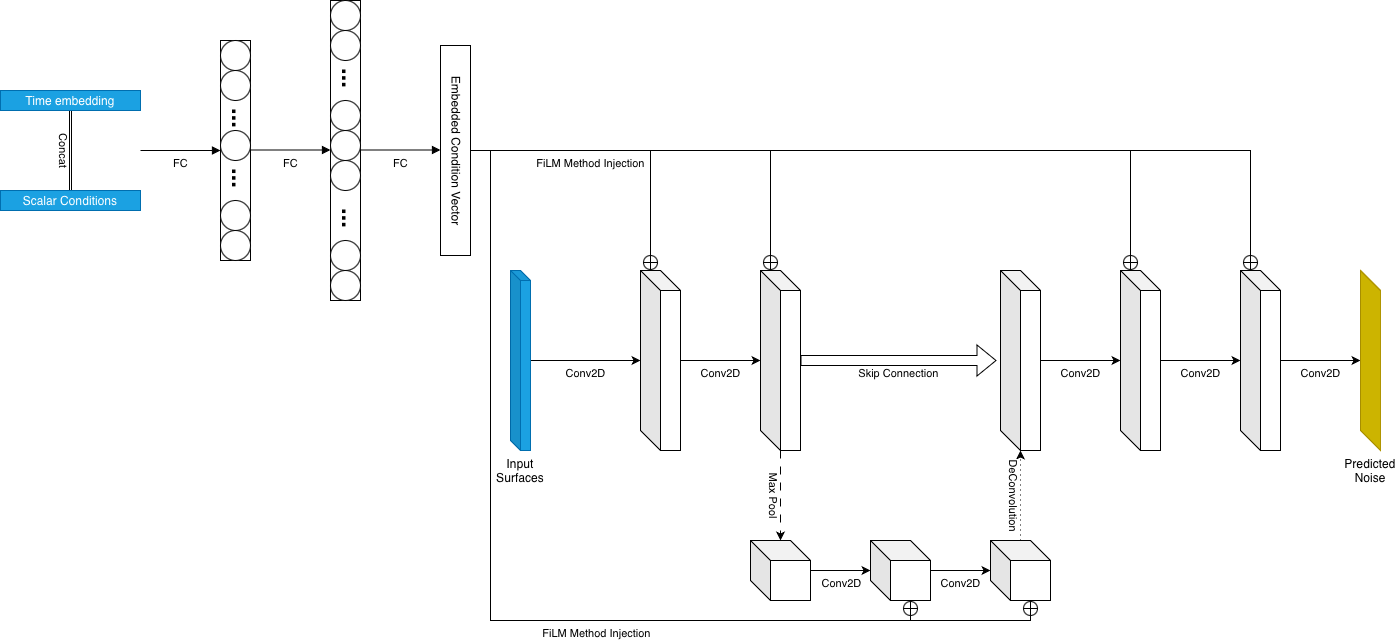
\includegraphics[width=0.9\textwidth]{fig/arch.png}
    \caption{Architecture of the diffusion model.}
    \label{fig:arch}
\end{figure}

For our specific implementation, the U-Net architecture is designed to map the 4-channel input tensor ($4 \times 9 \times 9$) to a single-channel output ($1 \times 9 \times 9$) representing the predicted noise. The encoder path begins with 16 encoding channels (\texttt{enc\_channels}), expanding to 30 channels (\texttt{bottle\_channels}) in the bottleneck. The sinusoidal time embedding and the scalar MLP each produce a 10-dimensional vector, which are concatenated to form a total 24-dimensional embedding (\texttt{emb\_dim}). The feed-forward network within the FiLM block that processes this joint embedding consists of 2 hidden layers with 10 neurons each, using a SiLU activation function. The 5 scalar conditioning features $\mathbf{c}^{(k)}$ are constructed using the $\alpha$ parameters $\alpha_{trend, short} = 0.156$, $\alpha_{trend, long} = 0.118$, $\alpha_{vol, short} = 0.3$, and $\alpha_{vol, long} = 0.15$, plus the daily VIX return.

\subsection{Training and Sampling Algorithm}

This subsection outlines the specific procedures for training the conditional U-Net model and subsequently using it to generate novel implied volatility surfaces, incorporating the arbitrage penalty.

\subsubsection{Loss Function}

The model is trained by minimizing a loss function $\mathcal{L}(\theta)$ with two goals: fidelity to the real data distribution and adherence to financial plausibility through no-arbitrage constraints. Simply adding a fixed arbitrage penalty to the standard Mean Squared Error (MSE) loss can lead to instabilities during training, primarily due to imbalance between the MSE loss and the arbitrage penalty term.

The loss function combines the standard Denoising Score Matching (DSM) objective with a dynamically weighted arbitrage penalty term:
\eqlnostar{eq:total_loss}{
\mathcal{L}(\theta) = \mathcal{L}_{\text{MSE}}(\theta) + \lambda \mathcal{L}_{\text{arb, weighted}}(\theta).
}
The \textbf{MSE Loss} term $\mathcal{L}_{\text{MSE}}(\theta)$ remains the standard objective focused on learning the data distribution by matching the noise added during the forward process:
\eqlnostar{eq:mse_loss}{
\mathcal{L}_{\text{MSE}}(\theta) = \mathbb{E}_{t, \mathbf{x}_0, \boldsymbol{\epsilon}, \mathbf{c}} \left[ || \boldsymbol{\epsilon} - \boldsymbol{\epsilon}_\theta(\mathbf{x}_t, t, \mathbf{c}) ||^2 \right],
}
where $\mathbf{x}_0 = \tilde{\mathbf{z}}^{(k)}$ is the normalized log-volatility surface, $\mathbf{x}_t$ is its noisy version at timestep $t \in \{1, ..., n\}$, $\boldsymbol{\epsilon} \sim \mathcal{N}(0, \mathbf{I})$ is the true noise, $\mathbf{c}$ is the conditioning vector, and $\boldsymbol{\epsilon}_\theta$ is the noise predicted by the U-Net. While alternative weighting schemes for the MSE loss exist, such as min-SNR weighting \citep{Hang_Gu_Li_Bao_Chen_Hu_Geng_Guo_2024}, our empirical results indicated that the standard, unweighted MSE loss \eqref{eq:mse_loss} performed better for this application and required less hyperparameter tuning.

The \textbf{Arbitrage Penalty} term, however, requires careful consideration. This penalty is applied to the model's estimate of the original clean surface, $\hat{\mathbf{x}}_0(\theta)$, obtained via denoising:
\eqlnostar{eq:denoised_estimate}{
\hat{\mathbf{x}}_0(\theta) = \frac{1}{\sqrt{\bar{\alpha}_t}} \left( \mathbf{x}_t - \sqrt{1 - \bar{\alpha}_t} \boldsymbol{\epsilon}_\theta(\mathbf{x}_t, t, \mathbf{c}) \right).
}
The reliability of this estimate $\hat{\mathbf{x}}_0$ varies significantly with the timestep $t$. When $t$ is large (i.e., at high noise levels, typically encountered early in the reverse diffusion process and frequently during training), $\mathbf{x}_t$ is mostly noise, and the resulting $\hat{\mathbf{x}}_0$ is a highly inaccurate approximation of the true $\mathbf{x}_0$. Applying the arbitrage penalty $\Phi$ (defined in Eqs. \ref{eq:penalty_calendar}-\ref{eq:penalty_butterfly}) to the corresponding volatility surface $\hat{\sigma} = \text{InvTransform}(\hat{\mathbf{x}}_0(\theta))$ in these high-noise regimes can yield large and potentially misleading penalty values. If this unreliably large penalty were added directly to the MSE loss with a fixed weight $\lambda$, it could easily overpower the MSE term, destabilizing training and diverting the model from accurately learning the underlying data distribution. The model might learn to produce noisy, low-arbitrage surfaces early on, hindering its ability to match the true data structure.

Conversely, when $t$ is small (low noise levels, encountered late in the reverse process and less frequently during uniform time sampling in training), the estimate $\hat{\mathbf{x}}_0$ is much closer to the true clean surface. Applying the arbitrage penalty in this regime is highly meaningful, as it directly encourages the final generated surface to satisfy no-arbitrage conditions. To dynamically balance the influence of the arbitrage penalty according to the reliability of the denoised estimate, we weight the penalty term by the Signal-to-Noise Ratio (SNR) at timestep $t$, defined as:
\eqlnostar{eq:snr_weight}{
w_{SNR}(t) = \frac{\bar{\alpha}_t}{1 - \bar{\alpha}_t + \epsilon_{stab}},
}
where $\epsilon_{stab}$ is a small constant (e.g., $10^{-8}$) for numerical stability. The SNR is inherently high when the signal component ($\sqrt{\bar{\alpha}_t} \mathbf{x}_0$) dominates (small $t$, low noise), and low when the noise component ($\sqrt{1 - \bar{\alpha}_t} \boldsymbol{\epsilon}$) dominates (large $t$, high noise). Multiplying the arbitrage penalty by $w_{SNR}(t)$ provides a natural weighting scheme: the penalty's contribution to the total loss is strongly emphasized when the denoised estimate is reliable (low $t$) and significantly down-weighted when the estimate is noisy and unreliable (high $t$). This prevents the potentially large and erratic penalties from high-noise steps from dominating the training objective, allowing the MSE term to guide the learning process effectively while still ensuring that the arbitrage constraints are strongly enforced as the generation process approaches the clean data manifold. The final \textbf{SNR-Weighted Arbitrage Loss} term is thus defined as:
\eqlnostar{eq:arb_loss_term_weighted}{
\mathcal{L}_{\text{arb, weighted}}(\theta) = \mathbb{E}_{t, \mathbf{x}_0, \boldsymbol{\epsilon}, \mathbf{c}} \left[ w_{SNR}(t) \cdot \Phi(\text{InvTransform}(\hat{\mathbf{x}}_0(\theta))) \right].
}
The hyperparameter $\lambda > 0$ in the total loss function \eqref{eq:total_loss} then sets the overall scale of this dynamically weighted arbitrage regularization relative to the primary data-fitting objective $\mathcal{L}_{\text{MSE}}$. It is worth noting that even when trained solely with the MSE loss ($\lambda=0$), the diffusion model demonstrated a capacity to generate visually plausible IV surfaces that largely respected the qualitative features expected in financial markets. This inherent structure-learning capability stands in contrast to Generative Adversarial Networks (GANs), which requires smooth function in the loss function to generate plausible surfaces. This observation suggests that DDPM is a potentially more robust choice for this application compared to GAN, even before the inclusion of explicit financial constraints. The calculation of the discrete finite differences required for the arbitrage penalties $p_1, p_2, p_3$ (Equations \eqref{eq:penalty_calendar}, \eqref{eq:penalty_callspread}, \eqref{eq:penalty_butterfly}) is implemented efficiently using 2D convolution operations with fixed, pre-defined kernels applied to the surface of relative call prices $c(m, \tau)$. For instance, first-order differences along the moneyness or tenor dimension can be computed using kernels like $[[-1, 1]]$ or $[[-1], [1]]$. Second-order differences, needed for the butterfly penalty $p_3$, can be computed using kernels like $[[1, -2, 1]]$. This convolutional approach leverages highly optimized routines available in deep learning libraries, making the penalty calculation computationally feasible during training.

\subsubsection{Training Algorithm}

The model is trained for a total of 2000 epochs using a batch size of 64. We employ a cosine beta schedule \citep{Nichol_Dhariwal_2021} with $N=500$ diffusion steps. The parameters $\theta$ of the U-Net $\boldsymbol{\epsilon}_\theta$ are learned by minimizing the composite loss $\mathcal{L}(\theta)$ \eqref{eq:total_loss} with the AdamW optimizer \citep{Loshchilov_Hutter_2019} and an initial learning rate of $3 \times 10^{-4}$. The learning rate is dynamically managed by a \texttt{ReduceLROnPlateau} scheduler, which reduces the rate by a factor of 0.8 if the validation loss does not improve for 300 epochs, down to a minimum learning rate of $1 \times 10^{-6}$. Figure \ref{fig:lr_curve} demonstrates the \texttt{ReduceLROnPlateau} learning rate schedule of the training process. To ensure training stability, we apply gradient clipping with a maximum $L2$-norm of 0.15. The limited number of data samples makes the model prone to overfitting. To prevent this, we implement an early stopping criterion based on the validation loss. Furthermore, we maintain an Exponential Moving Average (EMA) of the model's parameters, $\theta_{EMA}$, with a decay rate of $\beta_{EMA} = 0.995$. The arbitrage penalty weights used in the loss function are $\lambda_{\text{smile}} = 0.01$ and $\lambda_{\text{ttm}} = 0.01$. The training process is detailed in Algorithm \ref{alg:training_ema}. Figure \ref{fig:loss_curves} shows the loss curve of the training and validation process.

\begin{figure}[htbp]
    \centering
    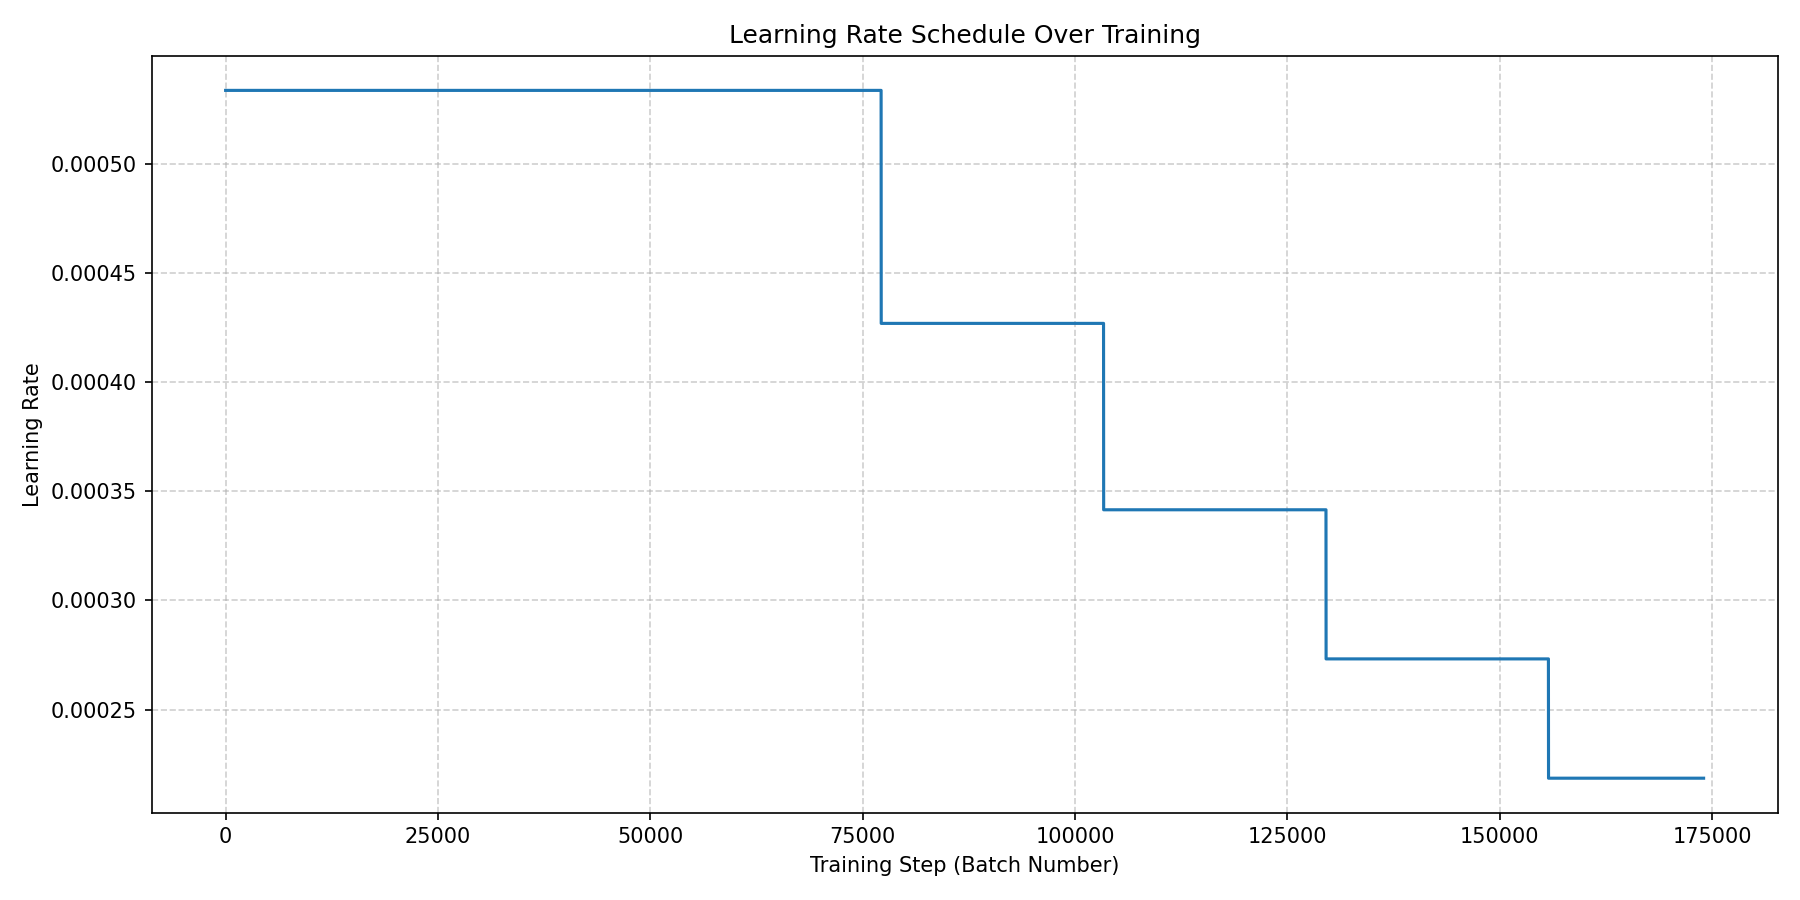
\includegraphics[width=0.9\textwidth]{fig/lr_curve.png}
    \caption{Learning rate schedule for the training process.}
    \label{fig:lr_curve}
\end{figure}

The parameters $\theta$ of the conditional U-Net $\boldsymbol{\epsilon}_\theta$ are learned by minimizing the composite loss $\mathcal{L}(\theta)$ using the AdamW optimizer \citep{Loshchilov_Hutter_2019}. The training process involves repeatedly sampling data points, timesteps, and noise, and updating the network weights based on the gradient of the loss. Crucially, the contribution of the arbitrage penalty to the total loss is weighted by the Signal-to-Noise Ratio (SNR) corresponding to the sampled timestep $t$, defined as $\text{SNR}(t) = \bar{\alpha}_t / (1 - \bar{\alpha}_t)$. This weighting scheme aims to balance the influence of the penalty across different noise levels during training. Additionally, following common practice, we maintain an Exponential Moving Average (EMA) of the model's parameters, denoted as $\theta_{EMA}$, using a decay rate $\beta_{EMA}$. This EMA is crucial for DDPM, the performance of EMA model and non-EMA model are dramatically different (we used EMA weight as 0.995). Algorithm \ref{alg:training_ema} provides the pseudocode for the training loop incorporating both SNR weighting and EMA updates.

\begin{figure}[htbp]
    \centering
    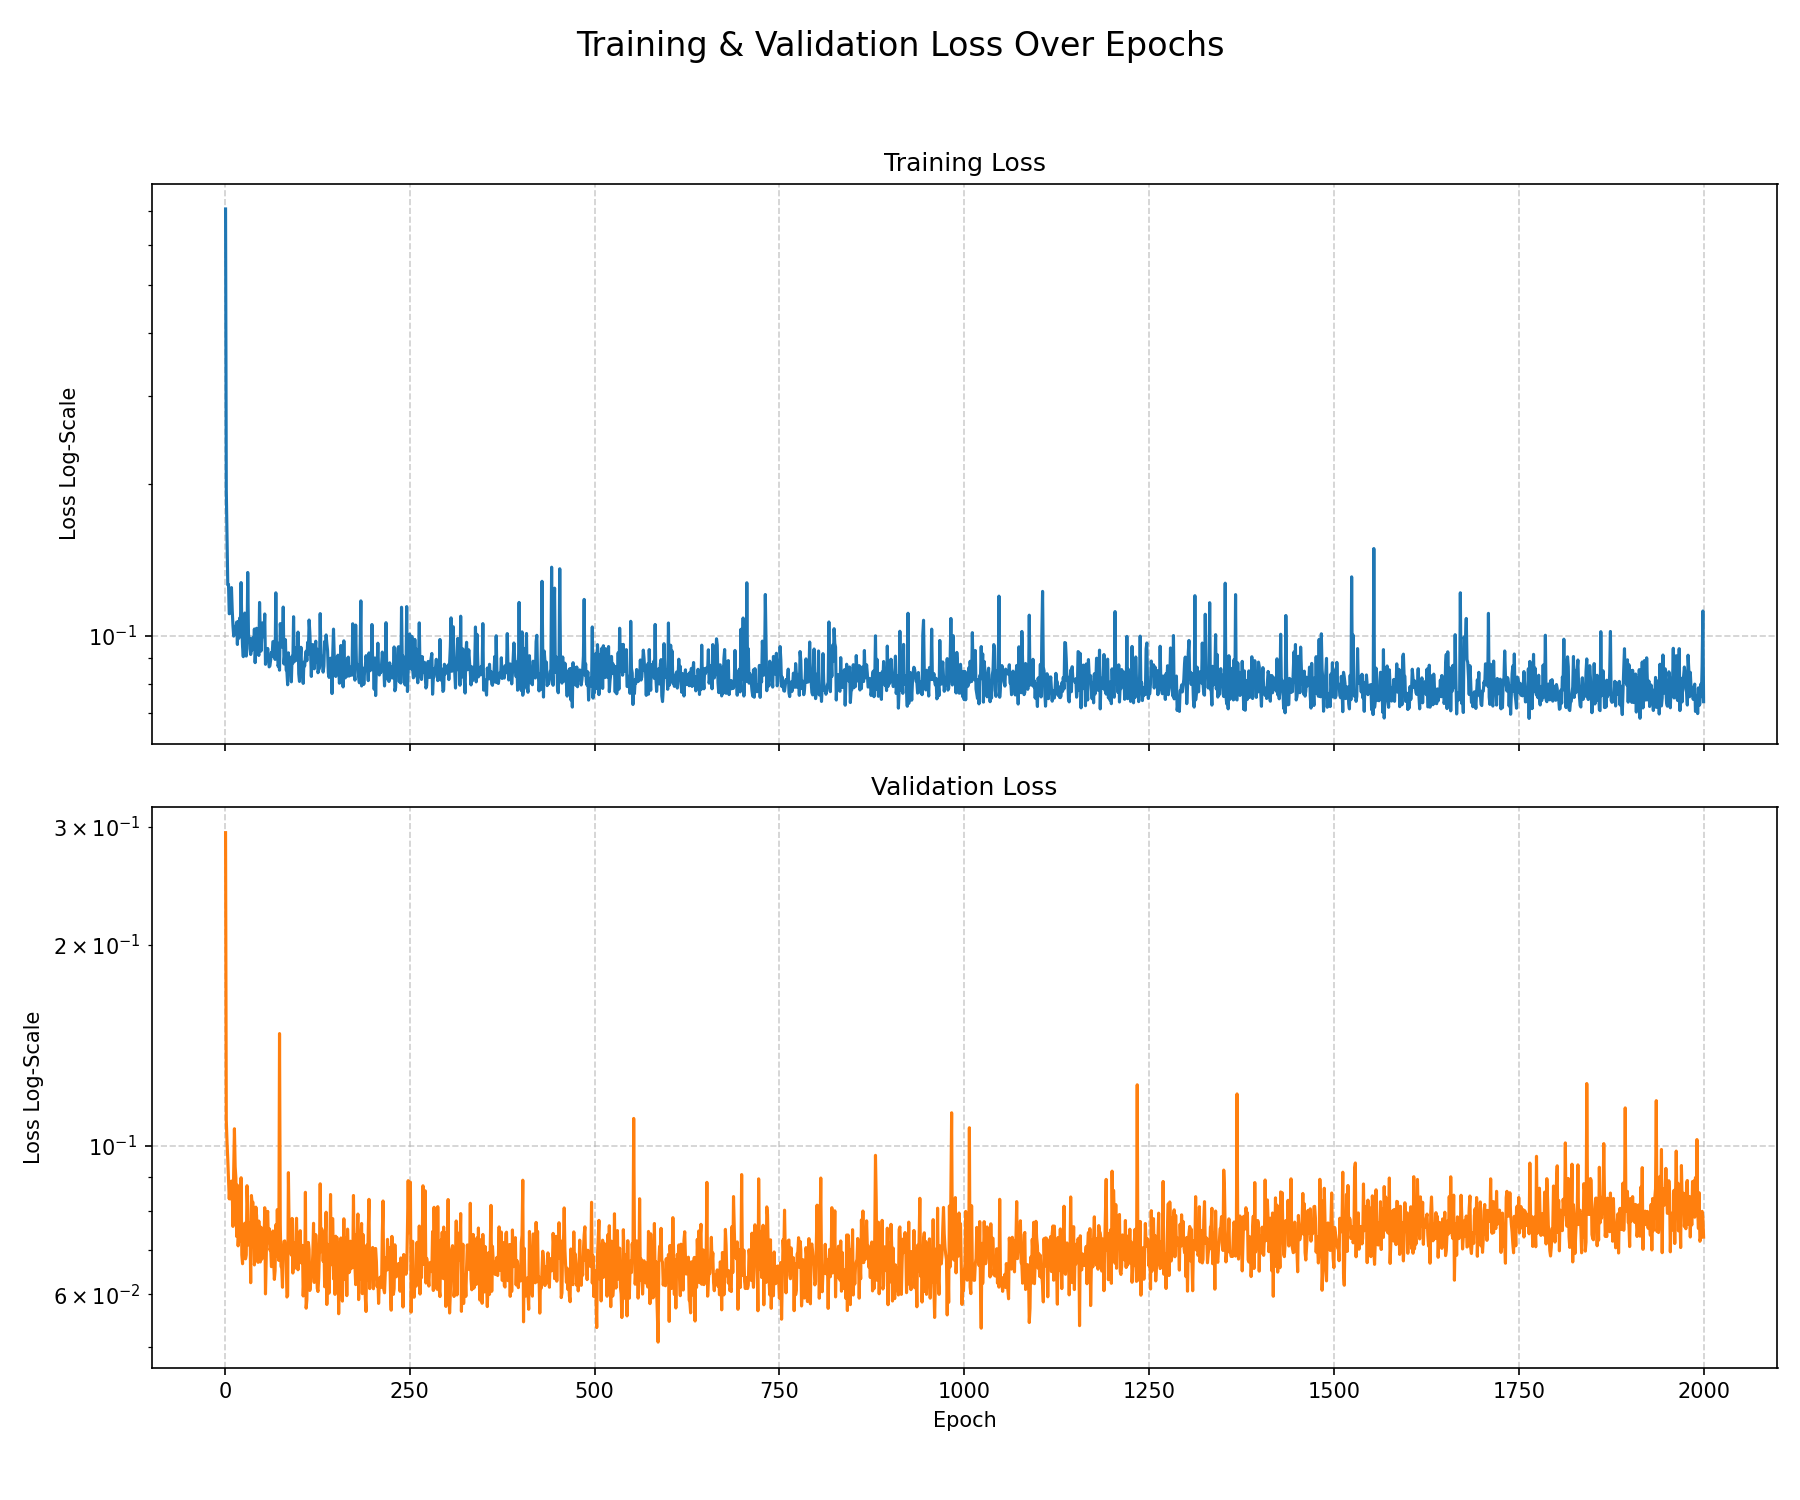
\includegraphics[width=0.9\textwidth]{fig/loss_curves.png}
    \caption{Loss curves of training and validation.}
    \label{fig:loss_curves}
\end{figure}

\begin{algorithm}[h!]
\caption{Training the Conditional Diffusion Model with SNR-Weighted Arbitrage Penalty and EMA}
\label{alg:training_ema}
\begin{algorithmic}[1]
\Require Training dataset $\{(\mathbf{x}_0^{(k)}, \mathbf{c}^{(k)})\}$ (normalized log-IV surfaces and conditions).
\Require Noise schedule $\{\beta_t\}_{t=1}^n$, derived quantities $\{\alpha_t, \bar{\alpha}_t\}_{t=1}^n$.
\Require Arbitrage penalty weight $\lambda$.
\Require Optimizer (e.g., AdamW), learning rate $\eta_{lr}$.
\Require EMA decay rate $\beta_{EMA}$ (e.g., 0.995).
\Require Number of training iterations $N_{iter}$.
\State Initialize model parameters $\theta$.
\State Initialize EMA parameters $\theta_{EMA} \leftarrow \theta$.
\For{iteration = 1 to $N_{iter}$}
    \State Sample a mini-batch of data $(\mathbf{x}_0, \mathbf{c})$ from the training set.
    \State Sample timestep $t \sim \text{Uniform}(\{1, ..., n\})$ for each sample.
    \State Sample noise $\boldsymbol{\epsilon} \sim \mathcal{N}(0, \mathbf{I})$.
    \State Compute noisy input: $\mathbf{x}_t = \sqrt{\bar{\alpha}_t} \mathbf{x}_0 + \sqrt{1 - \bar{\alpha}_t} \boldsymbol{\epsilon}$.
    \State Predict noise using the network with current parameters $\theta$: $\hat{\boldsymbol{\epsilon}}_\theta = \boldsymbol{\epsilon}_\theta(\mathbf{x}_t, t, \mathbf{c})$.
    \State Compute MSE loss: $L_{\text{MSE}} = || \boldsymbol{\epsilon} - \hat{\boldsymbol{\epsilon}}_\theta ||^2$ (averaged over mini-batch).
    \State Compute denoised estimate using current parameters $\theta$: $\hat{\mathbf{x}}_0 = \frac{1}{\sqrt{\bar{\alpha}_t}} ( \mathbf{x}_t - \sqrt{1 - \bar{\alpha}_t} \hat{\boldsymbol{\epsilon}}_\theta )$.
    \State Transform $\hat{\mathbf{x}}_0$ back to volatility scale: $\hat{\sigma} = \text{InvTransform}(\hat{\mathbf{x}}_0)$.
    \State Calculate arbitrage penalty $\Phi(\hat{\sigma})$ using convolutional kernels (per sample).
    \State Calculate SNR weight for each sample's timestep $t$: $w_{SNR}(t) = \bar{\alpha}_t / (1 - \bar{\alpha}_t + \epsilon_{stab})$ (where $\epsilon_{stab}$ is a small constant for stability).
    \State Compute total loss (averaged over mini-batch): $\mathcal{L} = L_{\text{MSE}} + \lambda \cdot \text{mean}(w_{SNR}(t) \cdot \Phi(\hat{\sigma}))$.
    \State Compute gradient $\nabla_\theta \mathcal{L}$.
    \State Update parameters using optimizer: $\theta \leftarrow \text{OptimizerStep}(\theta, \nabla_\theta \mathcal{L}, \eta_{lr})$.
    \State Update EMA parameters: $\theta_{EMA} \leftarrow \beta_{EMA} \cdot \theta_{EMA} + (1 - \beta_{EMA}) \cdot \theta$.
\EndFor
\State \Return Trained EMA parameters $\theta_{EMA}$.
\end{algorithmic}
\end{algorithm}

\subsubsection{Sampling Algorithm}

After training, the model with the stored EMA parameters $\theta_{EMA}$ is used to generate new IV surfaces conditioned on a specific context vector $\mathbf{c}$. This is achieved by simulating the reverse diffusion process, starting from pure Gaussian noise $\mathbf{x}_n \sim \mathcal{N}(0, \mathbf{I})$ and iteratively denoising it using the learned EMA model. We employ the standard DDPM sampling algorithm \citep{Ho_Jain_Abbeel_2020}, replacing the instantaneous model weights with the EMA weights, as detailed in Algorithm \ref{alg:sampling_ema}.
\begin{algorithm}[h!]
\caption{Sampling Conditional IV Surfaces using EMA Model}
\label{alg:sampling_ema}
\begin{algorithmic}[1]
\Require Trained EMA model parameters $\theta_{EMA}$.
\Require Conditioning vector $\mathbf{c}$ for the target day.
\Require Noise schedule $\{\alpha_t, \beta_t, \bar{\alpha}_t\}_{t=1}^n$.
\State Sample initial noise $\mathbf{x}_n \sim \mathcal{N}(0, \mathbf{I})$.
\For{$t = n, n-1, ..., 1$}
    \State Sample $\mathbf{z} \sim \mathcal{N}(0, \mathbf{I})$ if $t > 1$, else $\mathbf{z} = \mathbf{0}$.
    \State Predict noise using the EMA model: $\hat{\boldsymbol{\epsilon}}_{\theta_{EMA}} = \boldsymbol{\epsilon}_{\theta_{EMA}}(\mathbf{x}_t, t, \mathbf{c})$.
    \State Compute mean of the reverse conditional distribution $p_{\theta_{EMA}}(\mathbf{x}_{t-1}|\mathbf{x}_t)$:
           \[ \boldsymbol{\mu}_{\theta_{EMA}}(\mathbf{x}_t, t) = \frac{1}{\sqrt{\alpha_t}} \left( \mathbf{x}_t - \frac{\beta_t}{\sqrt{1-\bar{\alpha}_t}} \hat{\boldsymbol{\epsilon}}_{\theta_{EMA}} \right). \]
    \State Compute variance/standard deviation of the reverse step. A common choice is $\sigma_t^2 = \tilde{\beta}_t = \frac{1-\bar{\alpha}_{t-1}}{1-\bar{\alpha}_t} \beta_t$.
    \State Perform the reverse step (sample $\mathbf{x}_{t-1}$):
           \[ \mathbf{x}_{t-1} = \boldsymbol{\mu}_{\theta_{EMA}}(\mathbf{x}_t, t) + \sigma_t \mathbf{z}.
           \]
\EndFor
\State Obtain the final generated sample $\mathbf{x}_0$ (in normalized log-space).
\State Transform $\mathbf{x}_0$ back to the original IV scale: $\hat{\sigma} = \text{InvTransform}(\mathbf{x}_0)$.
\State \Return Generated IV surface $\hat{\sigma}$.
\end{algorithmic}
\end{algorithm}
This procedure allows for the generation of multiple, distinct IV surface samples for the same conditioning input $\mathbf{c}$, reflecting the inherent uncertainty in market dynamics, leveraging the stability benefits often provided by the EMA model weights.

\subsubsection{Epsilon-Prediction vs. V-Prediction and Output Clipping}
A technical detail in implementing diffusion models concerns the parameterization of the network's output and potential numerical stability issues, particularly near the beginning of the reverse process (when $t$ is small, corresponding to large $T-t$ in the SDE notation). In the standard epsilon-prediction formulation used throughout this paper (where the network predicts $\boldsymbol{\epsilon}_\theta$), calculating the denoised estimate $\hat{\mathbf{x}}_0$ \eqref{eq:denoised_estimate} or the mean of the reverse step $\boldsymbol{\mu}_\theta(\mathbf{x}_t, t)$ involves terms like $1/\sqrt{\bar{\alpha}_t}$ and $(1-\alpha_t)/\sqrt{1-\bar{\alpha}_t}$. As $t \to 0$, $\bar{\alpha}_t \to 1$, but $\alpha_t$ also approaches 1. However, the term $\sqrt{1-\bar{\alpha}_t}$ in the denominator approaches zero, potentially causing these coefficients to explode numerically. This can lead to instability during sampling. A common practical workaround is to clip the calculated mean $\boldsymbol{\mu}_\theta(\mathbf{x}_t, t)$ or the denoised estimate $\hat{\mathbf{x}}_0$ to a pre-defined range (e.g., [-1, 1] if the data was normalized to this range) to prevent extreme values.

An alternative approach, known as v-prediction \citep{Salimans_Ho_2022}, reparameterizes the prediction target to circumvent this issue. Instead of predicting $\boldsymbol{\epsilon}$, the network is trained to predict $\mathbf{v} = \sqrt{\bar{\alpha}_t} \boldsymbol{\epsilon} - \sqrt{1-\bar{\alpha}_t} \mathbf{x}_0$. This target often has better scaling properties across the full range of $t$, particularly near $t=0$ and $t=n$, potentially leading to more stable training and sampling without the need for explicit clipping. The denoising and reverse step equations are adjusted accordingly based on the predicted $\mathbf{v}$.

While v-prediction offers theoretical advantages in terms of stability, our empirical investigations for modelling implied volatility surfaces found that the standard epsilon-prediction approach, combined with output clipping for the reverse step mean $\boldsymbol{\mu}_\theta(\mathbf{x}_t, t)$, yielded results largely comparable to those obtained using v-prediction. Given this similarity in performance for our specific application, we opted for the epsilon-prediction framework due to its slightly simpler formulation and widespread use.

\section{Result and Forecasting Performance}
\label{sec:performance}

This section evaluates the performance of the proposed conditional diffusion model. We assess the quality of the generated implied volatility surfaces against the test set and compare its capabilities to a benchmark VolGAN model. 

The VolGAN model is structured as a Conditional Generative Adversarial Network (CGAN). Its generator is conditioned on historical market data, the previous day's IV surface and recent underlying returns, and is trained to output a realistic one-day-ahead increment of the log-IV surface, along with the underlying's return. VolGAN's approach to handling arbitrage during training is a major difference. The model does not use an explicit, direct arbitrage penalty in its loss function. Instead, it incorporates a ``smoothness penalty'' (a discrete Sobolev semi-norm) into the generator's loss. This penalty encourages the model to produce regular, smooth surfaces, which indirectly reduces arbitrage violations that often stem from irregular shapes.

The evaluation focuses on quantitative accuracy, financial plausibility, and the model's ability to capture the distributional and structural properties of the IV manifold. Since the VolGAN model has instability issue, we are using the most accurate model among 9 trained models.

\subsection{Qualitative Plausibility of Generated Surfaces}
We should examine two key stylized facts on the surfaces: the volatility smile (non-linear curvature across moneyness) and the term structure (the shape across time to maturity). The surfaces should be free of any non-financial artifacts. Figure \ref{fig:qualitative_comparison} presents a side-by-side comparison (January 5, 2022) from the test set. It displays the real surface, the mean surface generated by our conditional diffusion model, and the mean surface generated by the benchmark VolGAN model, all for the same conditioning data.
\begin{figure}[h!]
    \centering
    \begin{subfigure}[b]{0.32\textwidth}
        \centering
        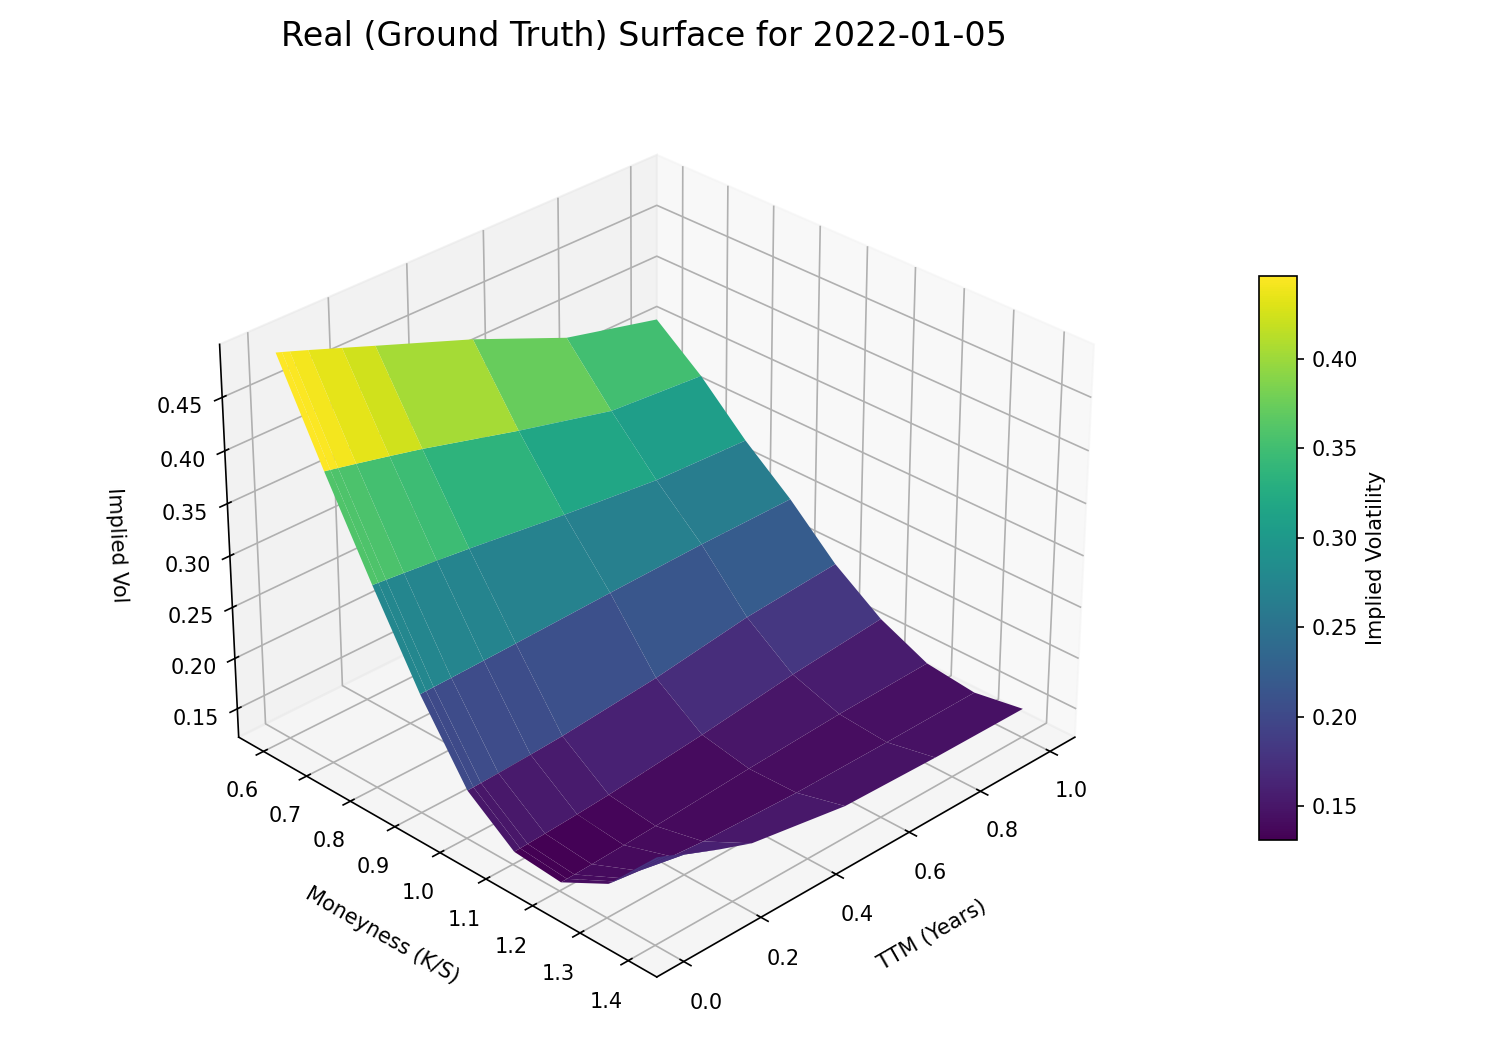
\includegraphics[width=\textwidth]{fig/REAL_surface_20220105.png}
        \caption{Real (Ground Truth).}
        \label{fig:real_surf}
    \end{subfigure}
    \hfill
    \begin{subfigure}[b]{0.32\textwidth}
        \centering
        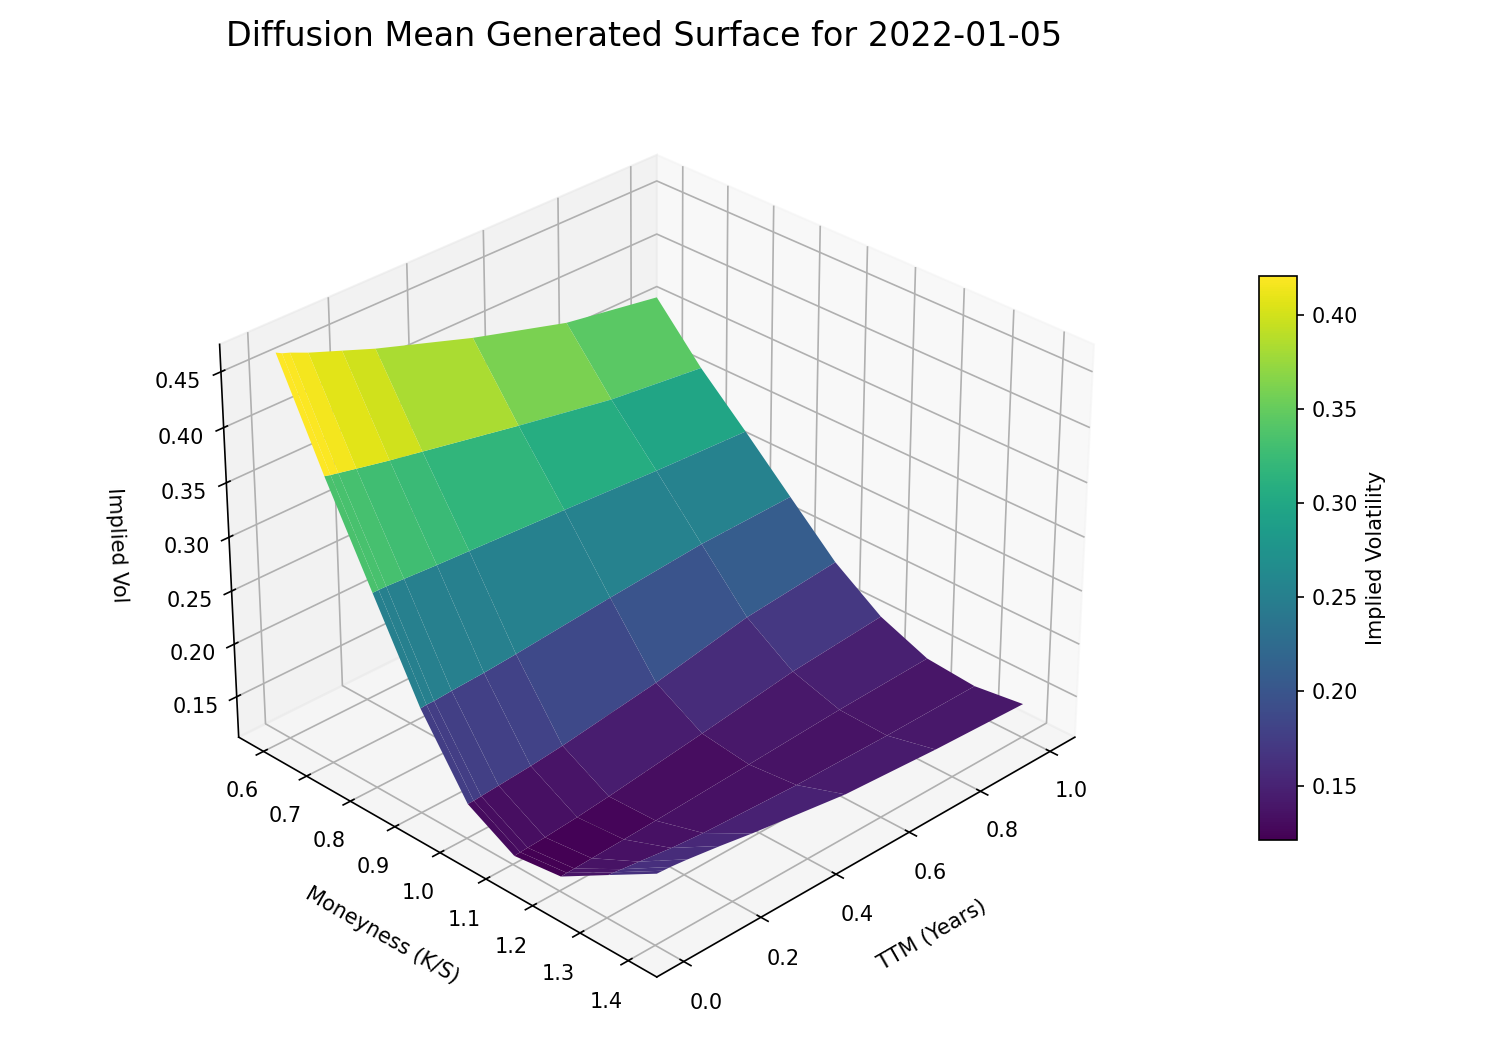
\includegraphics[width=\textwidth]{fig/DIFFUSION_MEAN_surface_20220105.png}
        \caption{Diffusion Model (Mean).}
        \label{fig:diff_surf}
    \end{subfigure}
    \hfill
    \begin{subfigure}[b]{0.32\textwidth}
        \centering
        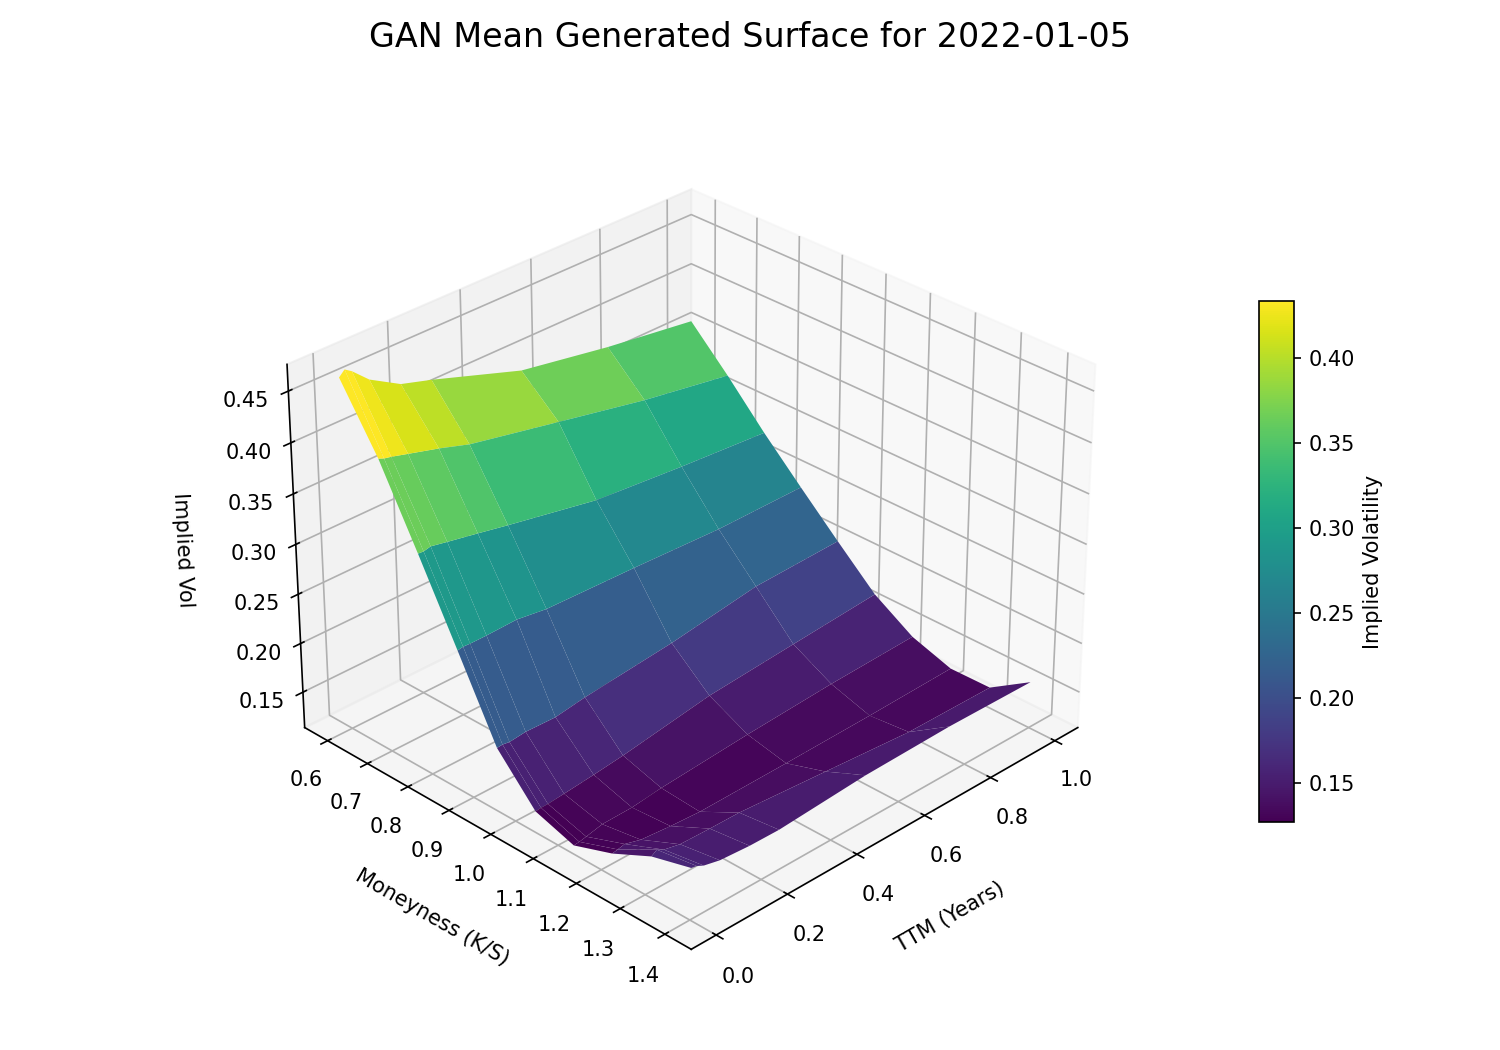
\includegraphics[width=\textwidth]{fig/GAN_MEAN_surface_20220105.png}
        \caption{VolGAN (Mean).}
        \label{fig:gan_surf}
    \end{subfigure}
    \caption{Qualitative comparison of generated surfaces for a single test-set date (2022-01-05). The (a) real surface shows a smooth, pronounced smirk. This shape is (b) closely replicated by our diffusion model, while (c) the VolGAN surface exhibits a "crease" at the short-term, low-moneyness corner.}
    \label{fig:qualitative_comparison}
\end{figure}
The ground truth surface in Panel (a) exhibits a classic volatility ``smirk'', with implied volatility peaking at low moneyness (deep OTM puts) and reaching a minimum near-the-money. The entire surface is smooth and continuous. Panel (b) shows the mean surface generated by our proposed diffusion model. Visually, it provides an excellent qualitative fit. The model accurately replicates the sharp curvature of the smile, including the steep wing at low moneyness, and the entire surface remains smooth and well-behaved, consistent with the real data. Panel (c) displays the mean surface from the VolGAN benchmark. While it captures the general shape of the smile, at the front corner, corresponding to low moneyness and low time-to-maturity, the surface displays a sharp ``crease'' or ``lip'' that is not present in the real data. This artifact suggests the GAN struggled to correctly learn the manifold's boundary constraints, resulting in an unstable or financially implausible shape in this region. Figure \ref{fig:qualitative_comparison} suggests that the diffusion model is more effective at learning and replicating the complex, smooth geometry of the implied volatility manifold.

\subsection{Quantitative Check of Generated Surfaces}
The qualitative inspection in the previous section suggests our model generates more plausible surfaces, this section provides a rigorous quantitative assessment of its point-wise forecasting accuracy and the reliability estimates. We analyze the model's performance over the entire test set and directly compare it to the VolGAN benchmark.

\paragraph{Time Series Slice Analysis.} We first analyze the models' forecasting performance beyond a static snapshot as a time series. For each day in the test set, we generate 100 conditional surfaces using both our diffusion model and the VolGAN, allowing us to compute a mean forecast and a 90\% confidence interval. The lower and upper bound are defined by the 5th and 95th percentiles of the samples, respectively.

Figures \ref{fig:atm_slices}, \ref{fig:itm_slices}, and \ref{fig:otm_slices} plot these time series results for seven representative points on the IV grid: At-the-Money (ATM) 1-Day, 1-Month, and 3-Month options; In-the-Money (ITM) 1-Month and 3-Month options; and Out-of-the-Money (OTM) 1-Month and 3-Month options. For each slice, we present a direct comparison between our Diffusion Model's forecast (left panel) and the VolGAN benchmark's forecast (right panel). Both plots overlay the model's mean prediction and 90\% confidence interval against the same ground truth (actual) IV data.
% --- FIGURE 1: ATM SLICES ---
\begin{figure}[h!]
    \centering
    \caption{Time series comparison for At-the-Money (ATM) slices. Left: Diffusion Model vs. Real. Right: VolGAN vs. Real.}
    \label{fig:atm_slices}

    % --- ATM 1-Day ---
    \begin{subfigure}[b]{0.49\textwidth}
        \centering
        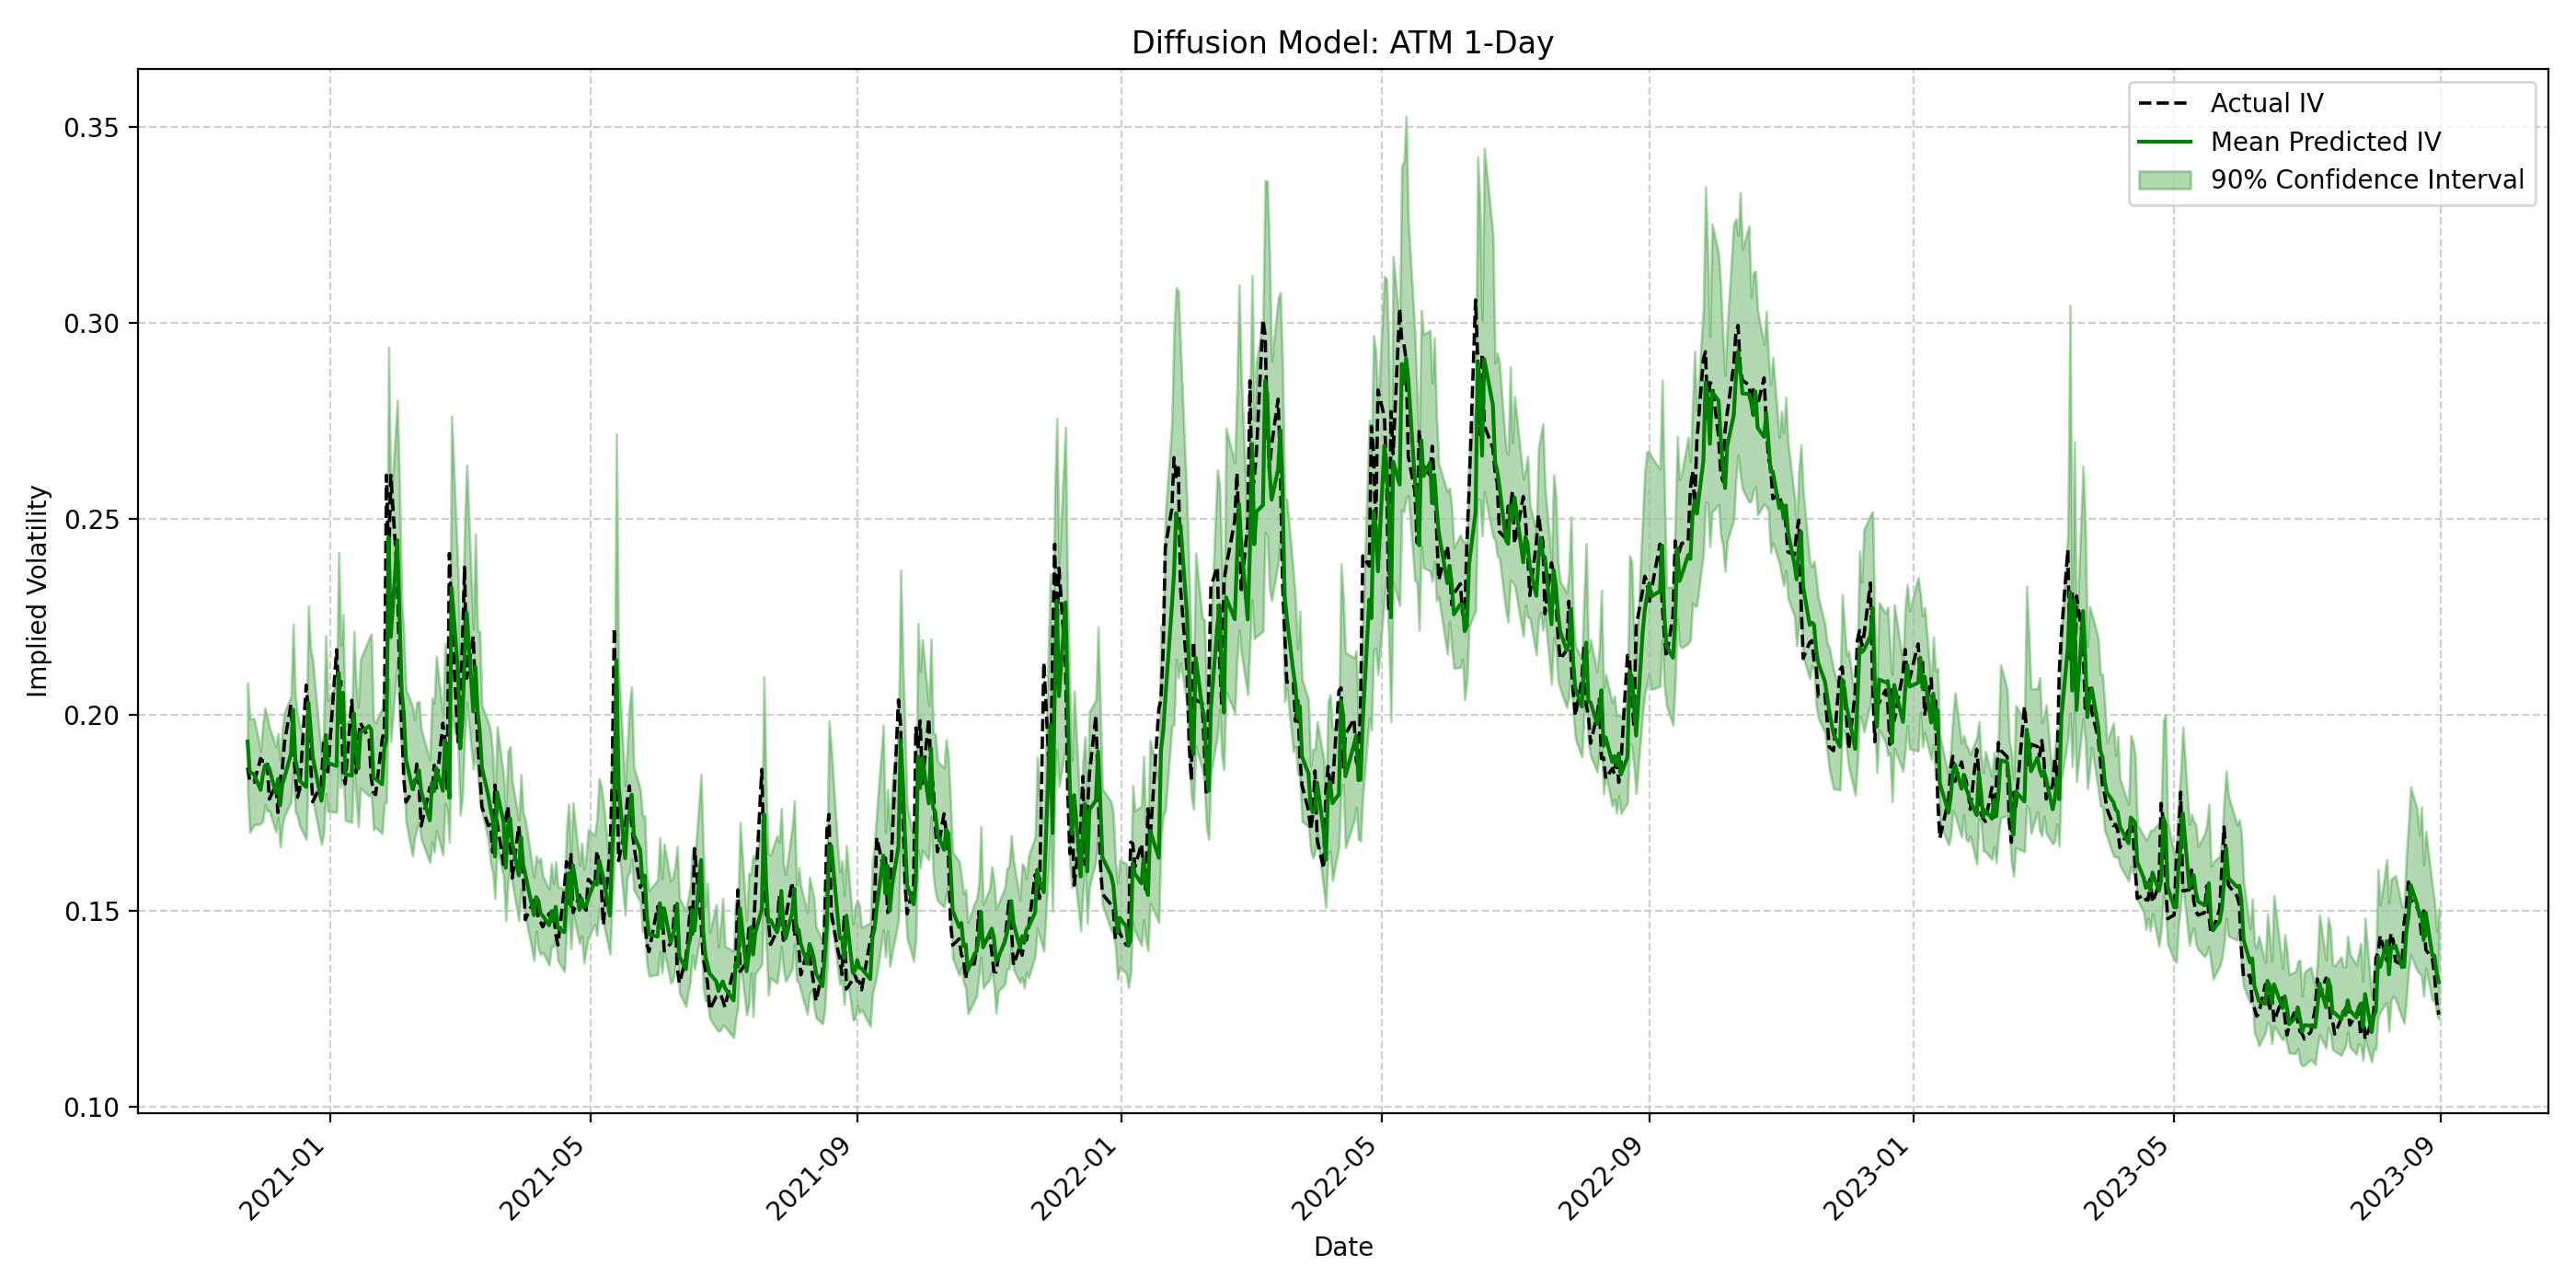
\includegraphics[width=\textwidth]{ts_slice/DiffusionModel_ATM_1-Day_comparison.png}
        \caption{Diffusion Model (ATM 1-Day).}
    \end{subfigure}
    \hfill
    \begin{subfigure}[b]{0.49\textwidth}
        \centering
        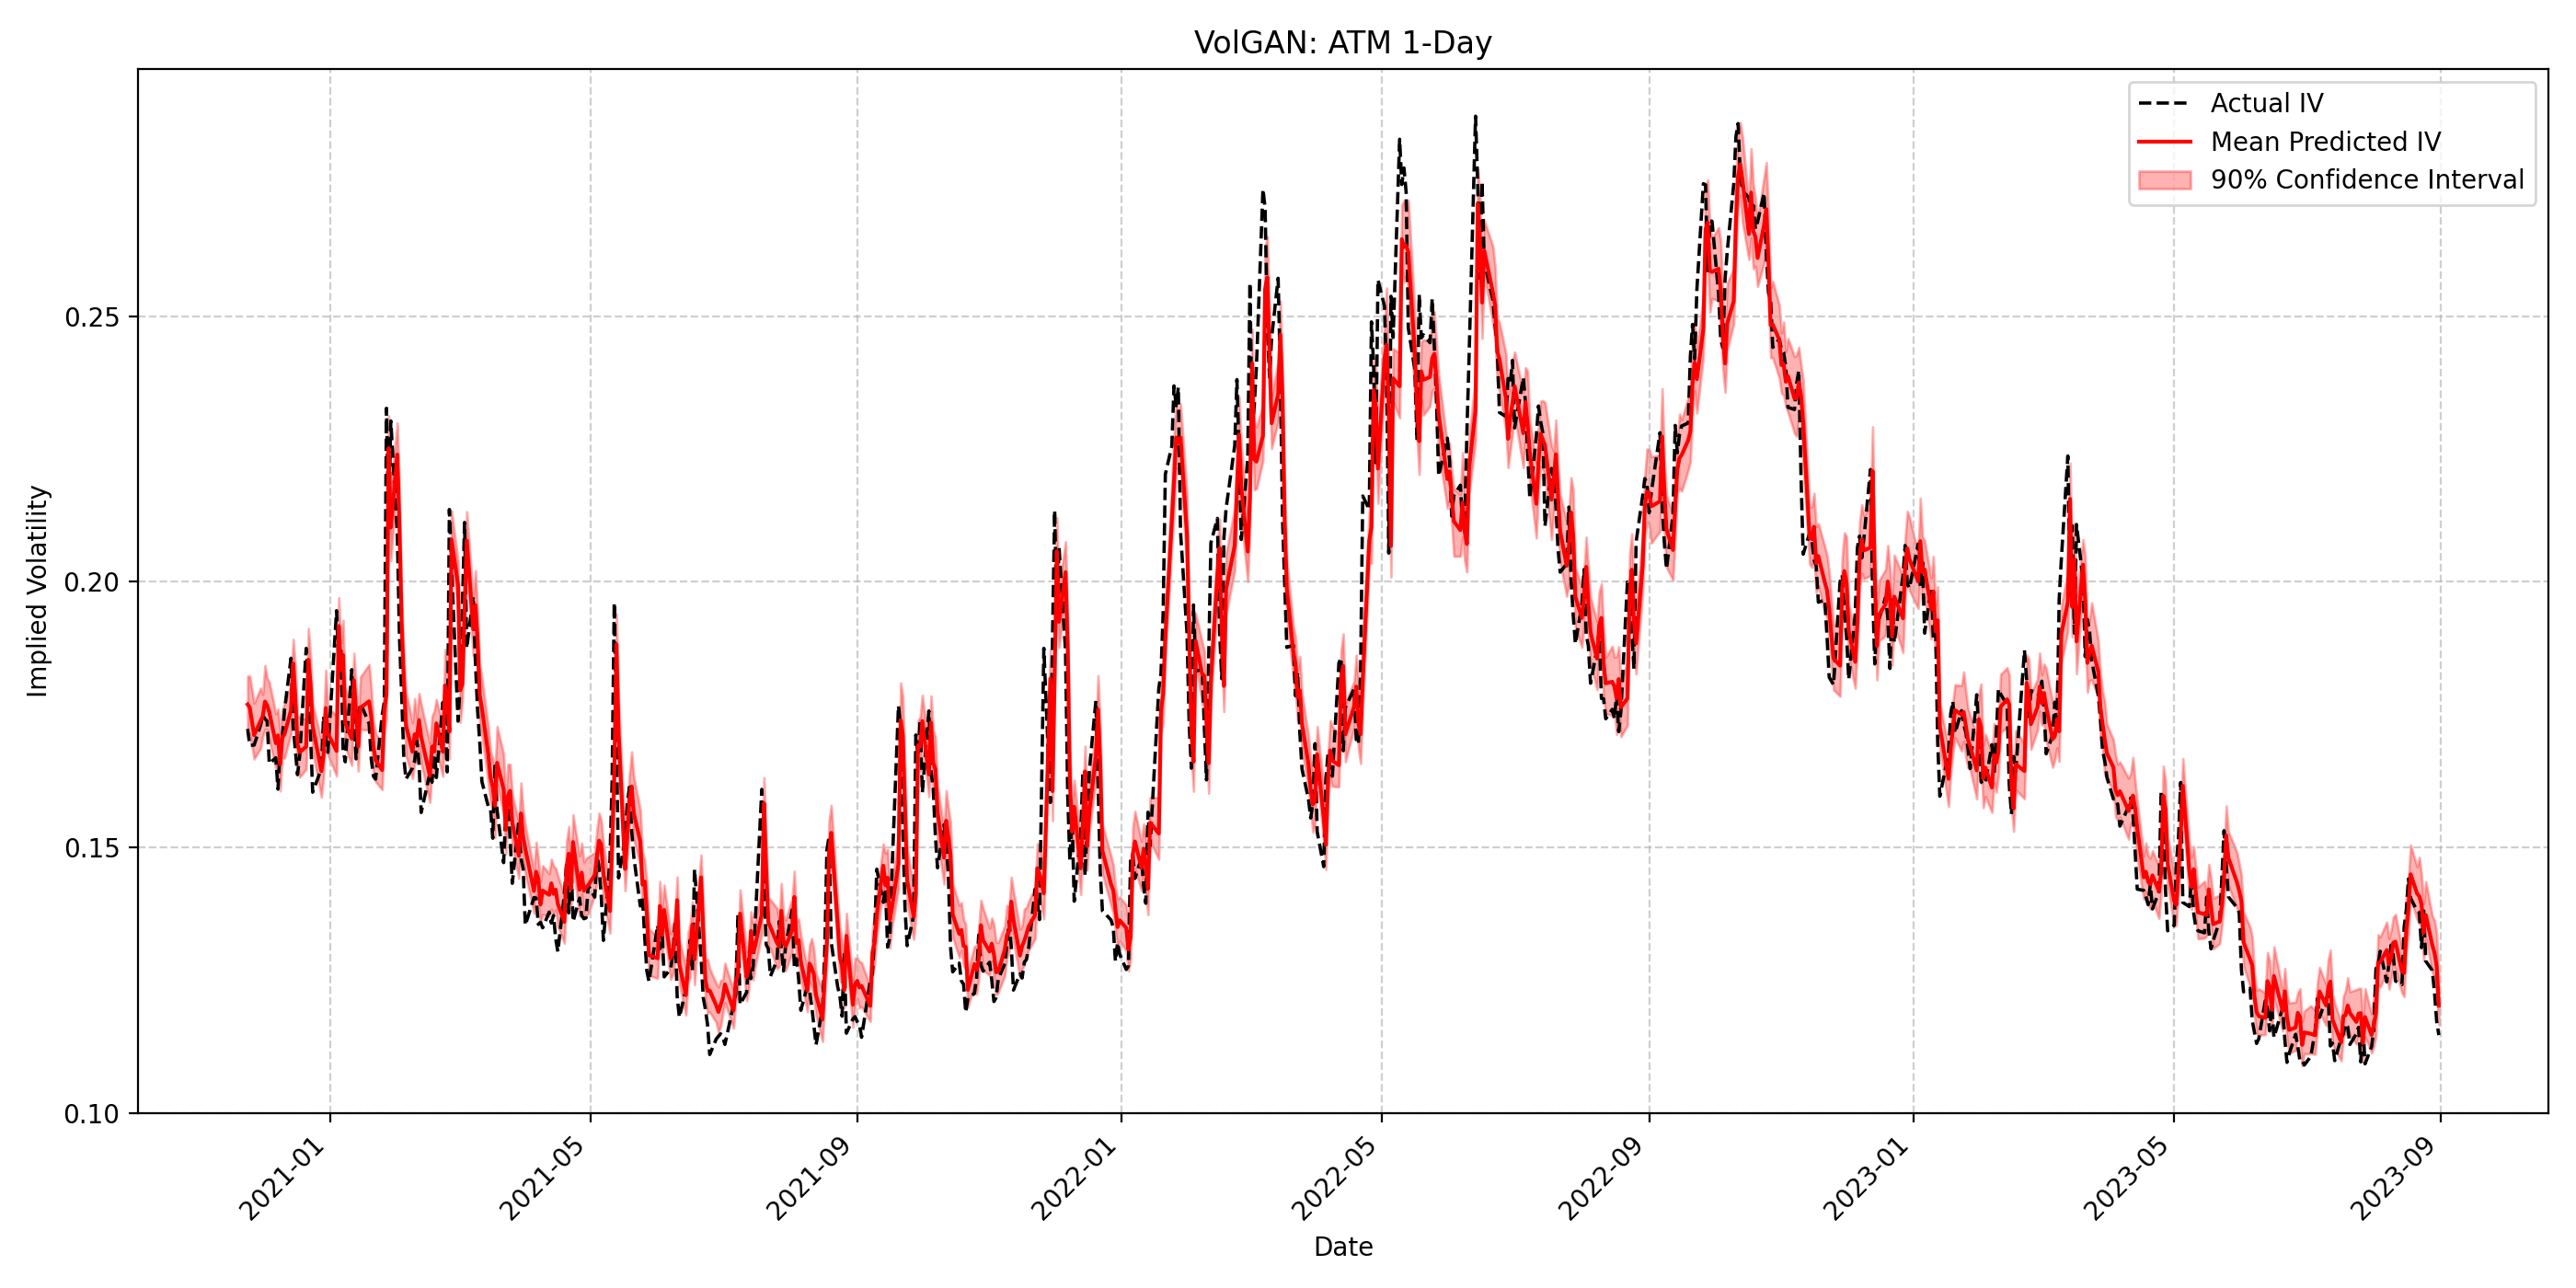
\includegraphics[width=\textwidth]{ts_slice/volgan_atm_1-day_ci.png}
        \caption{VolGAN Model (ATM 1-Day).}
    \end{subfigure}

    \vspace{0.5cm}
    
    % --- ATM 1-Month ---
    \begin{subfigure}[b]{0.49\textwidth}
        \centering
        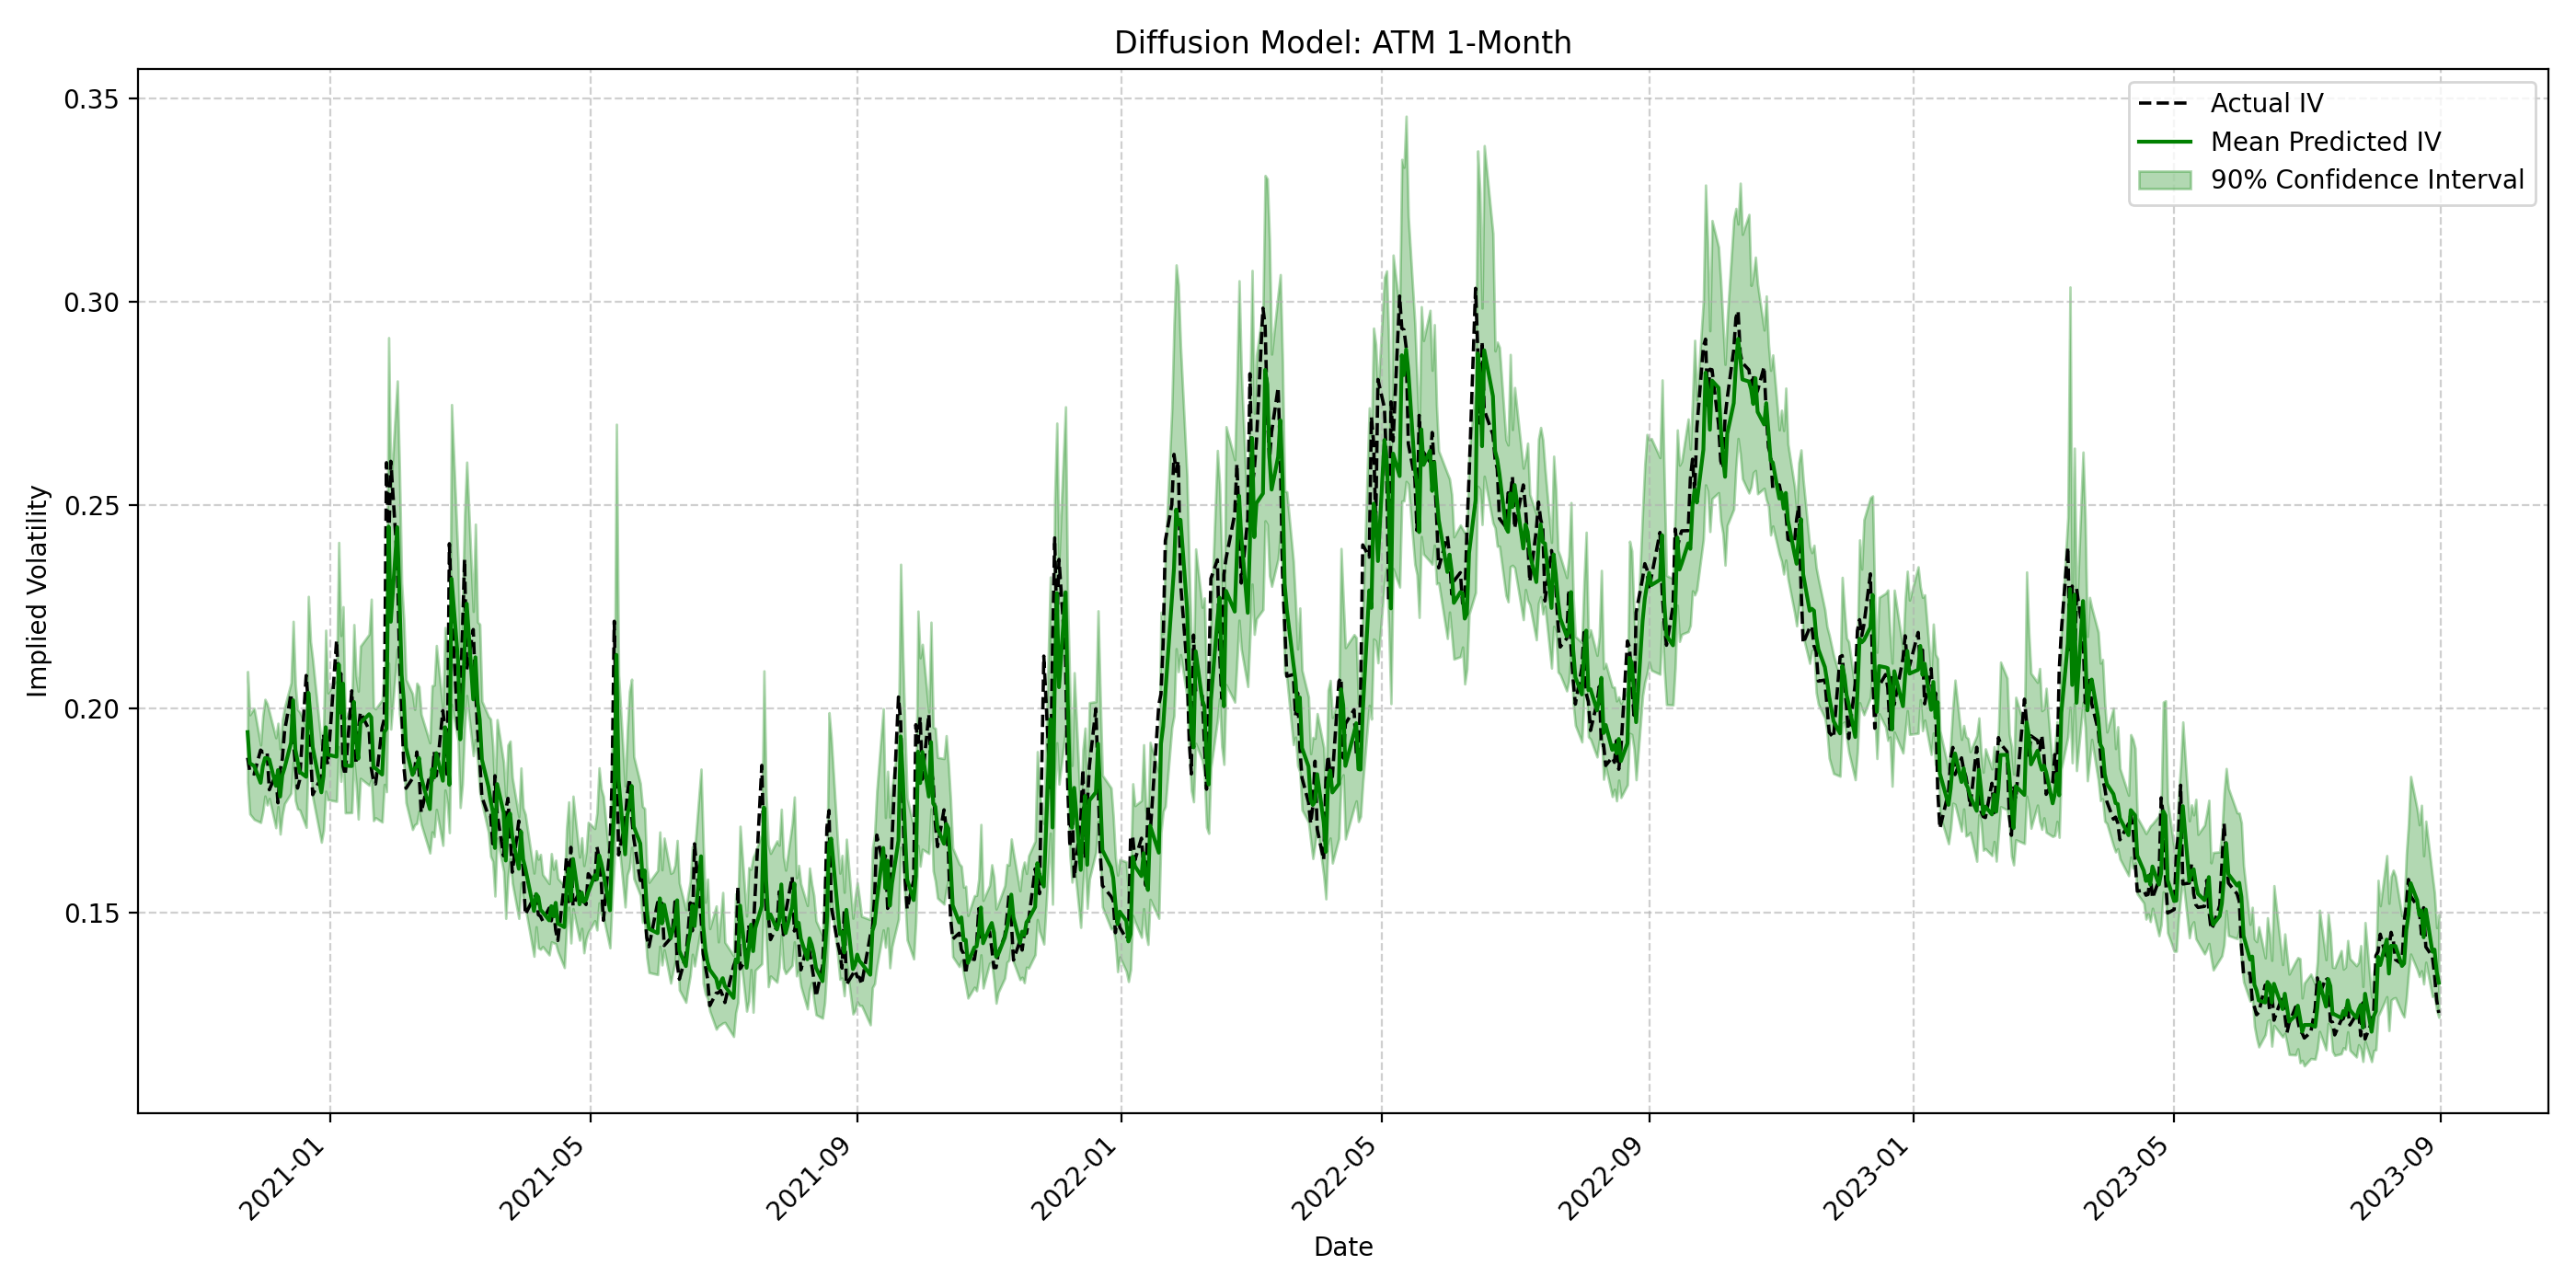
\includegraphics[width=\textwidth]{ts_slice/DiffusionModel_ATM_1-Month_comparison.png}
        \caption{Diffusion Model (ATM 1-Month).}
    \end{subfigure}
    \hfill
    \begin{subfigure}[b]{0.49\textwidth}
        \centering
        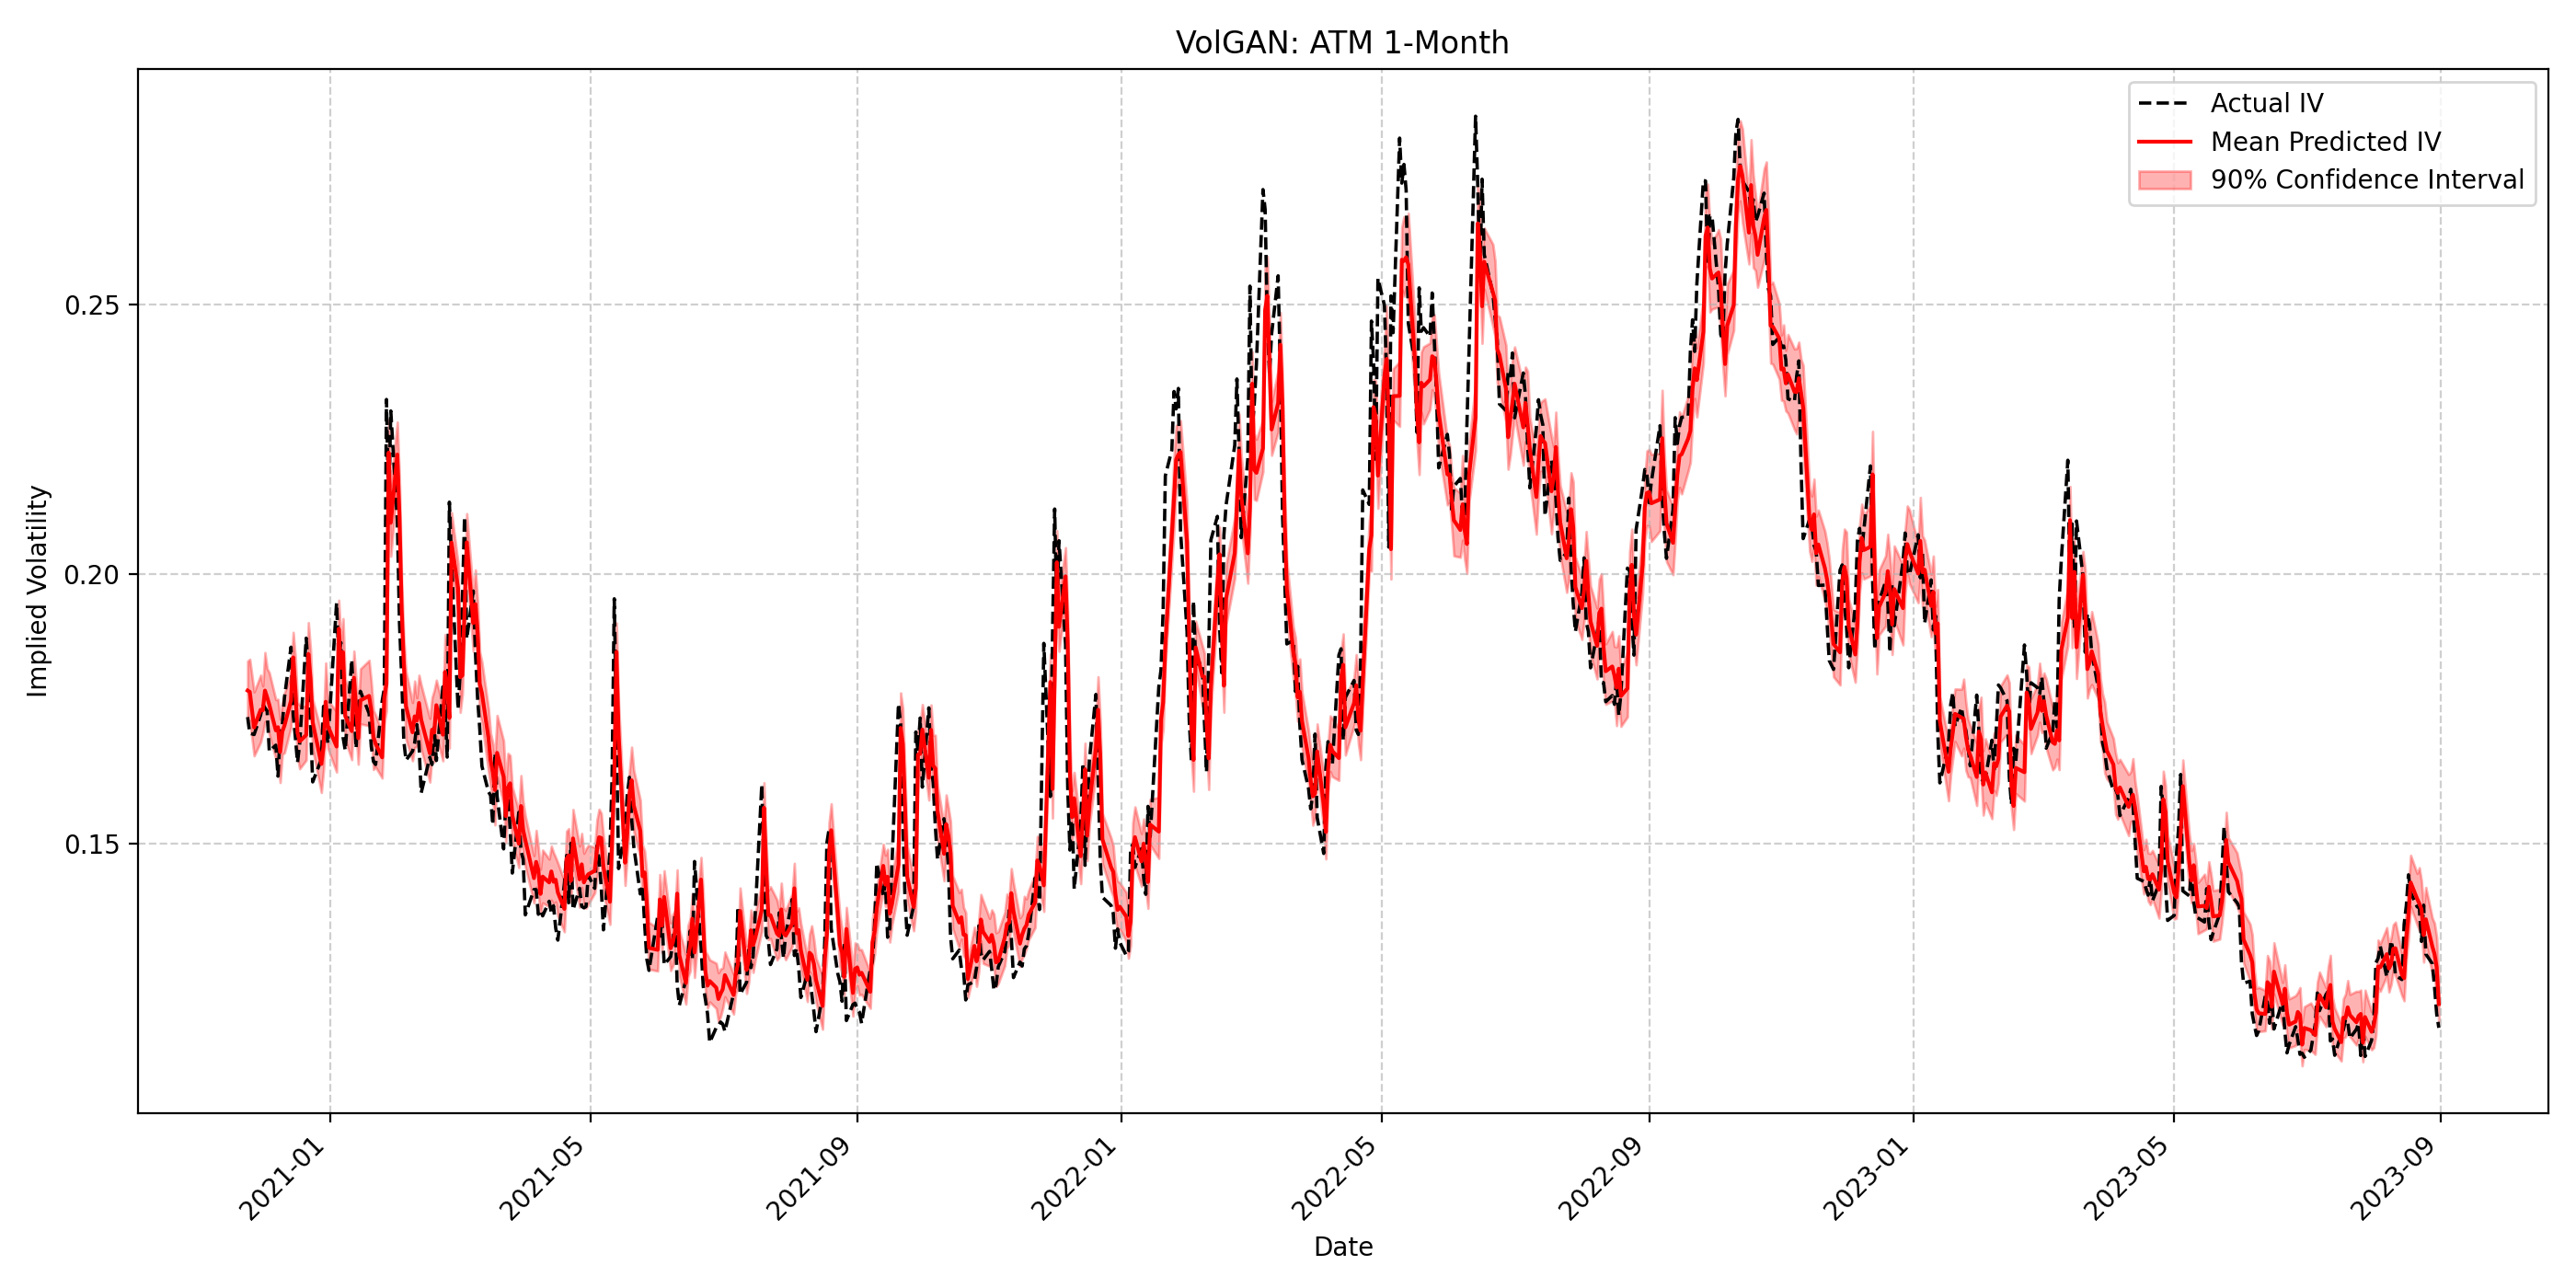
\includegraphics[width=\textwidth]{ts_slice/volgan_atm_1-month_ci.png}
        \caption{VolGAN Model (ATM 1-Month).}
    \end{subfigure}
    
    \vspace{0.5cm}

    % --- ATM 3-Month ---
    \begin{subfigure}[b]{0.49\textwidth}
        \centering
        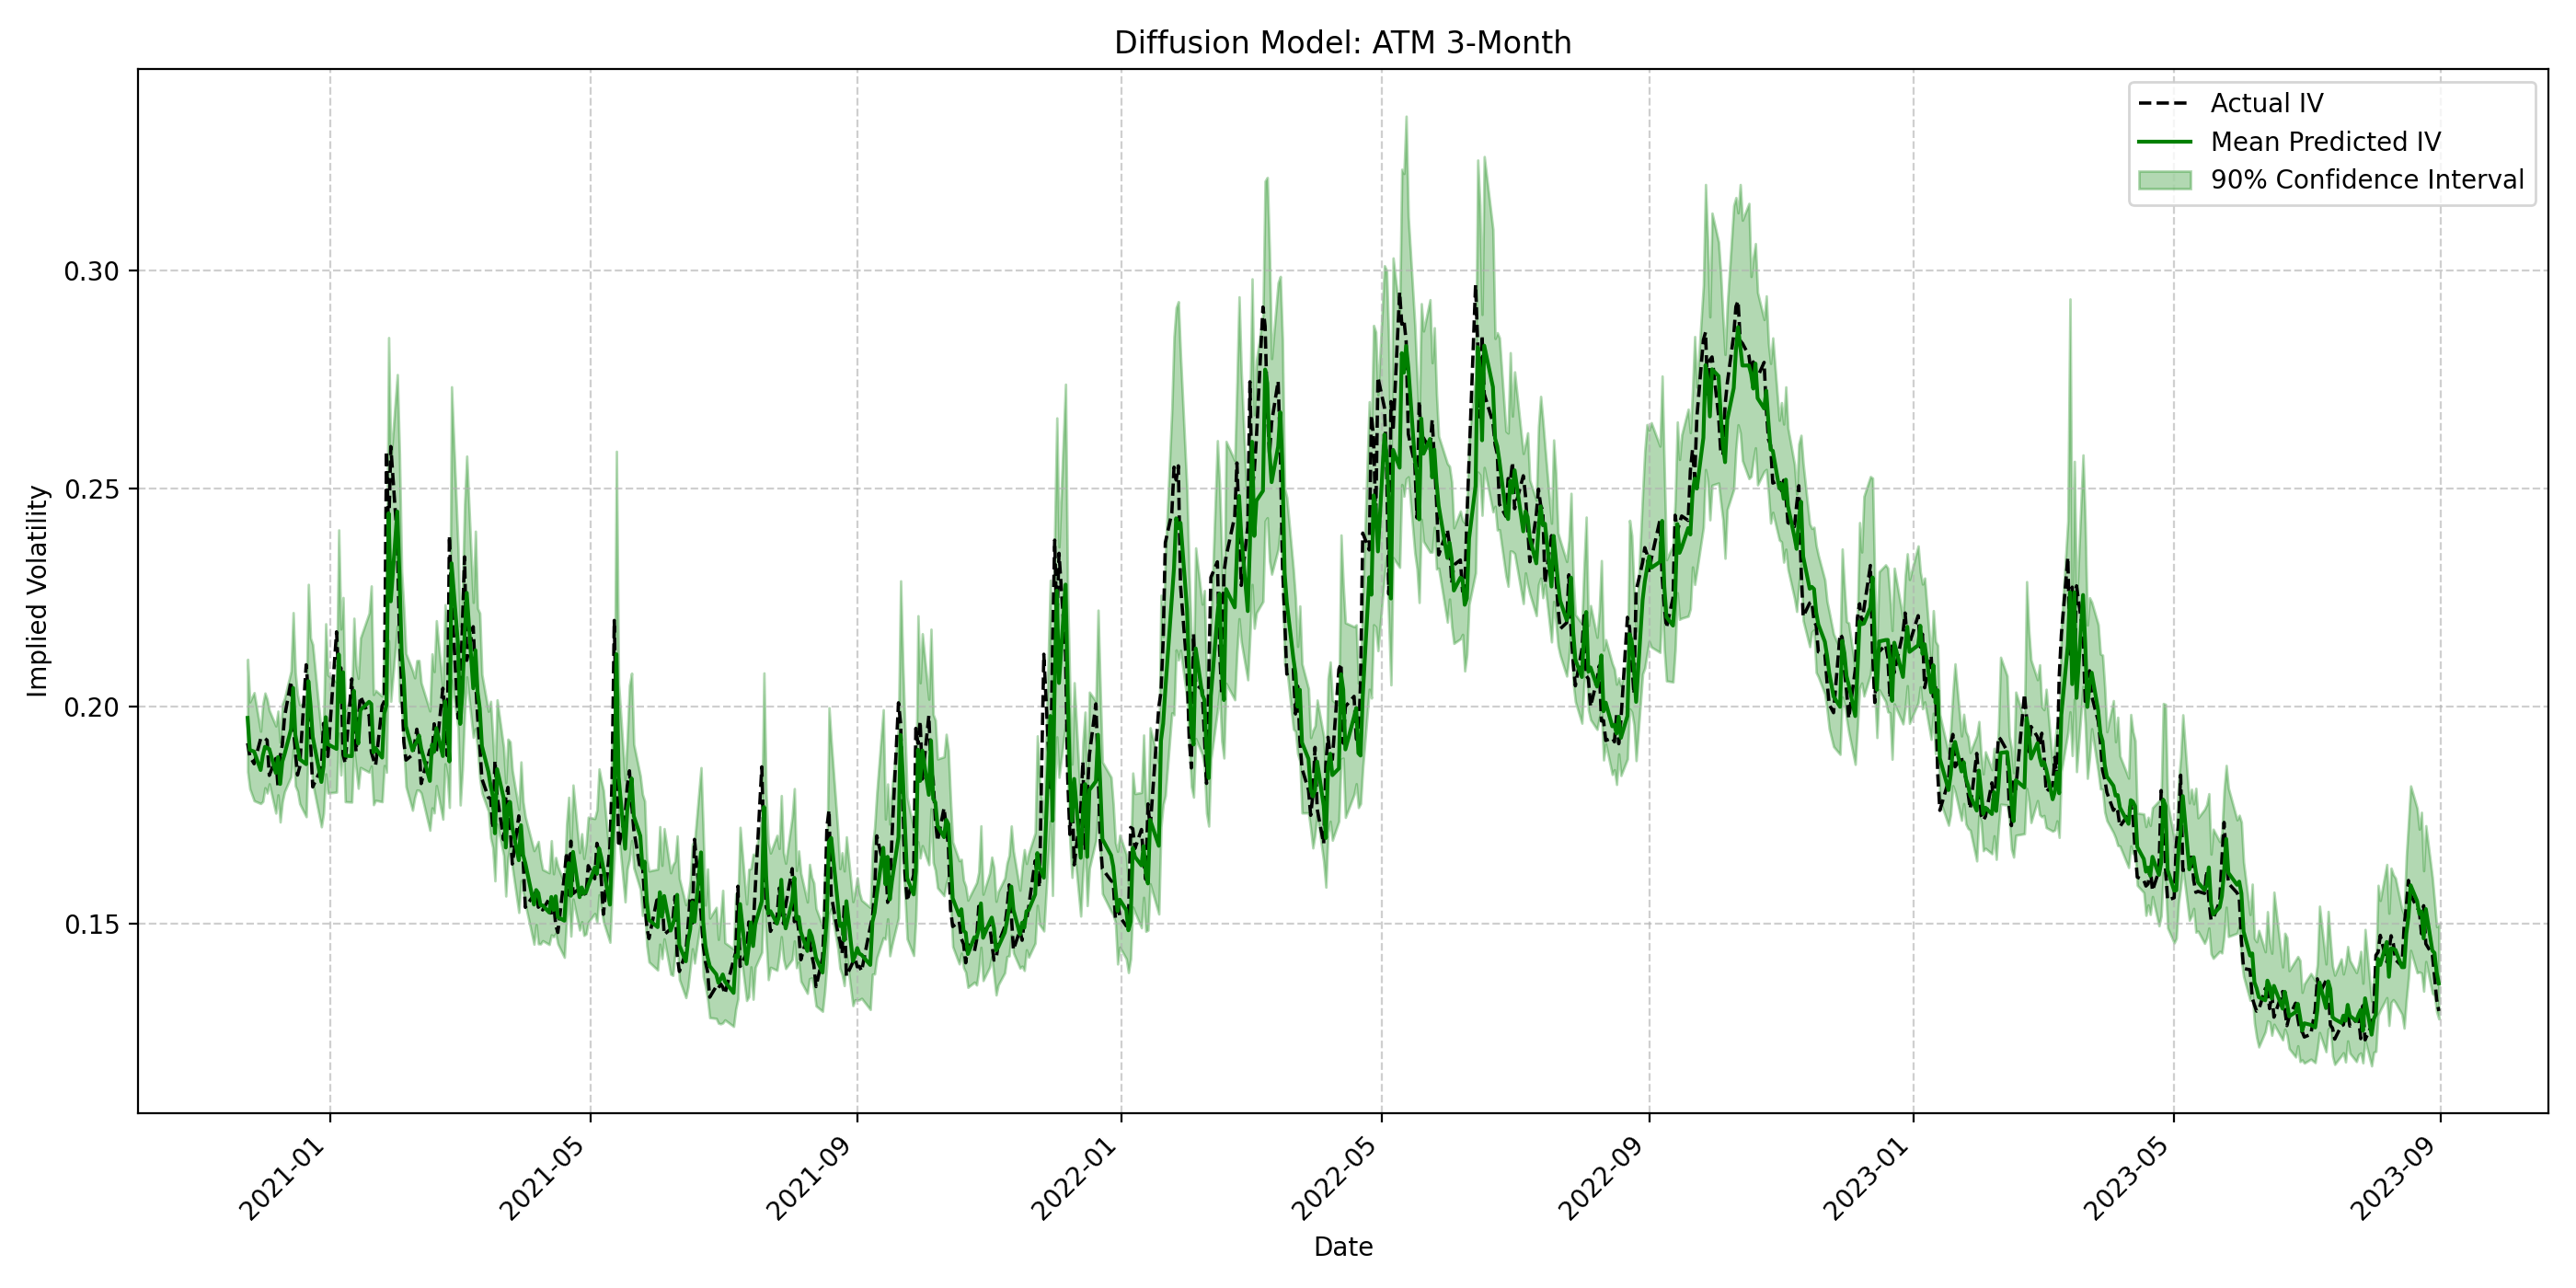
\includegraphics[width=\textwidth]{ts_slice/DiffusionModel_ATM_3-Month_comparison.png}
        \caption{Diffusion Model (ATM 3-Month).}
    \end{subfigure}
    \hfill
    \begin{subfigure}[b]{0.49\textwidth}
        \centering
        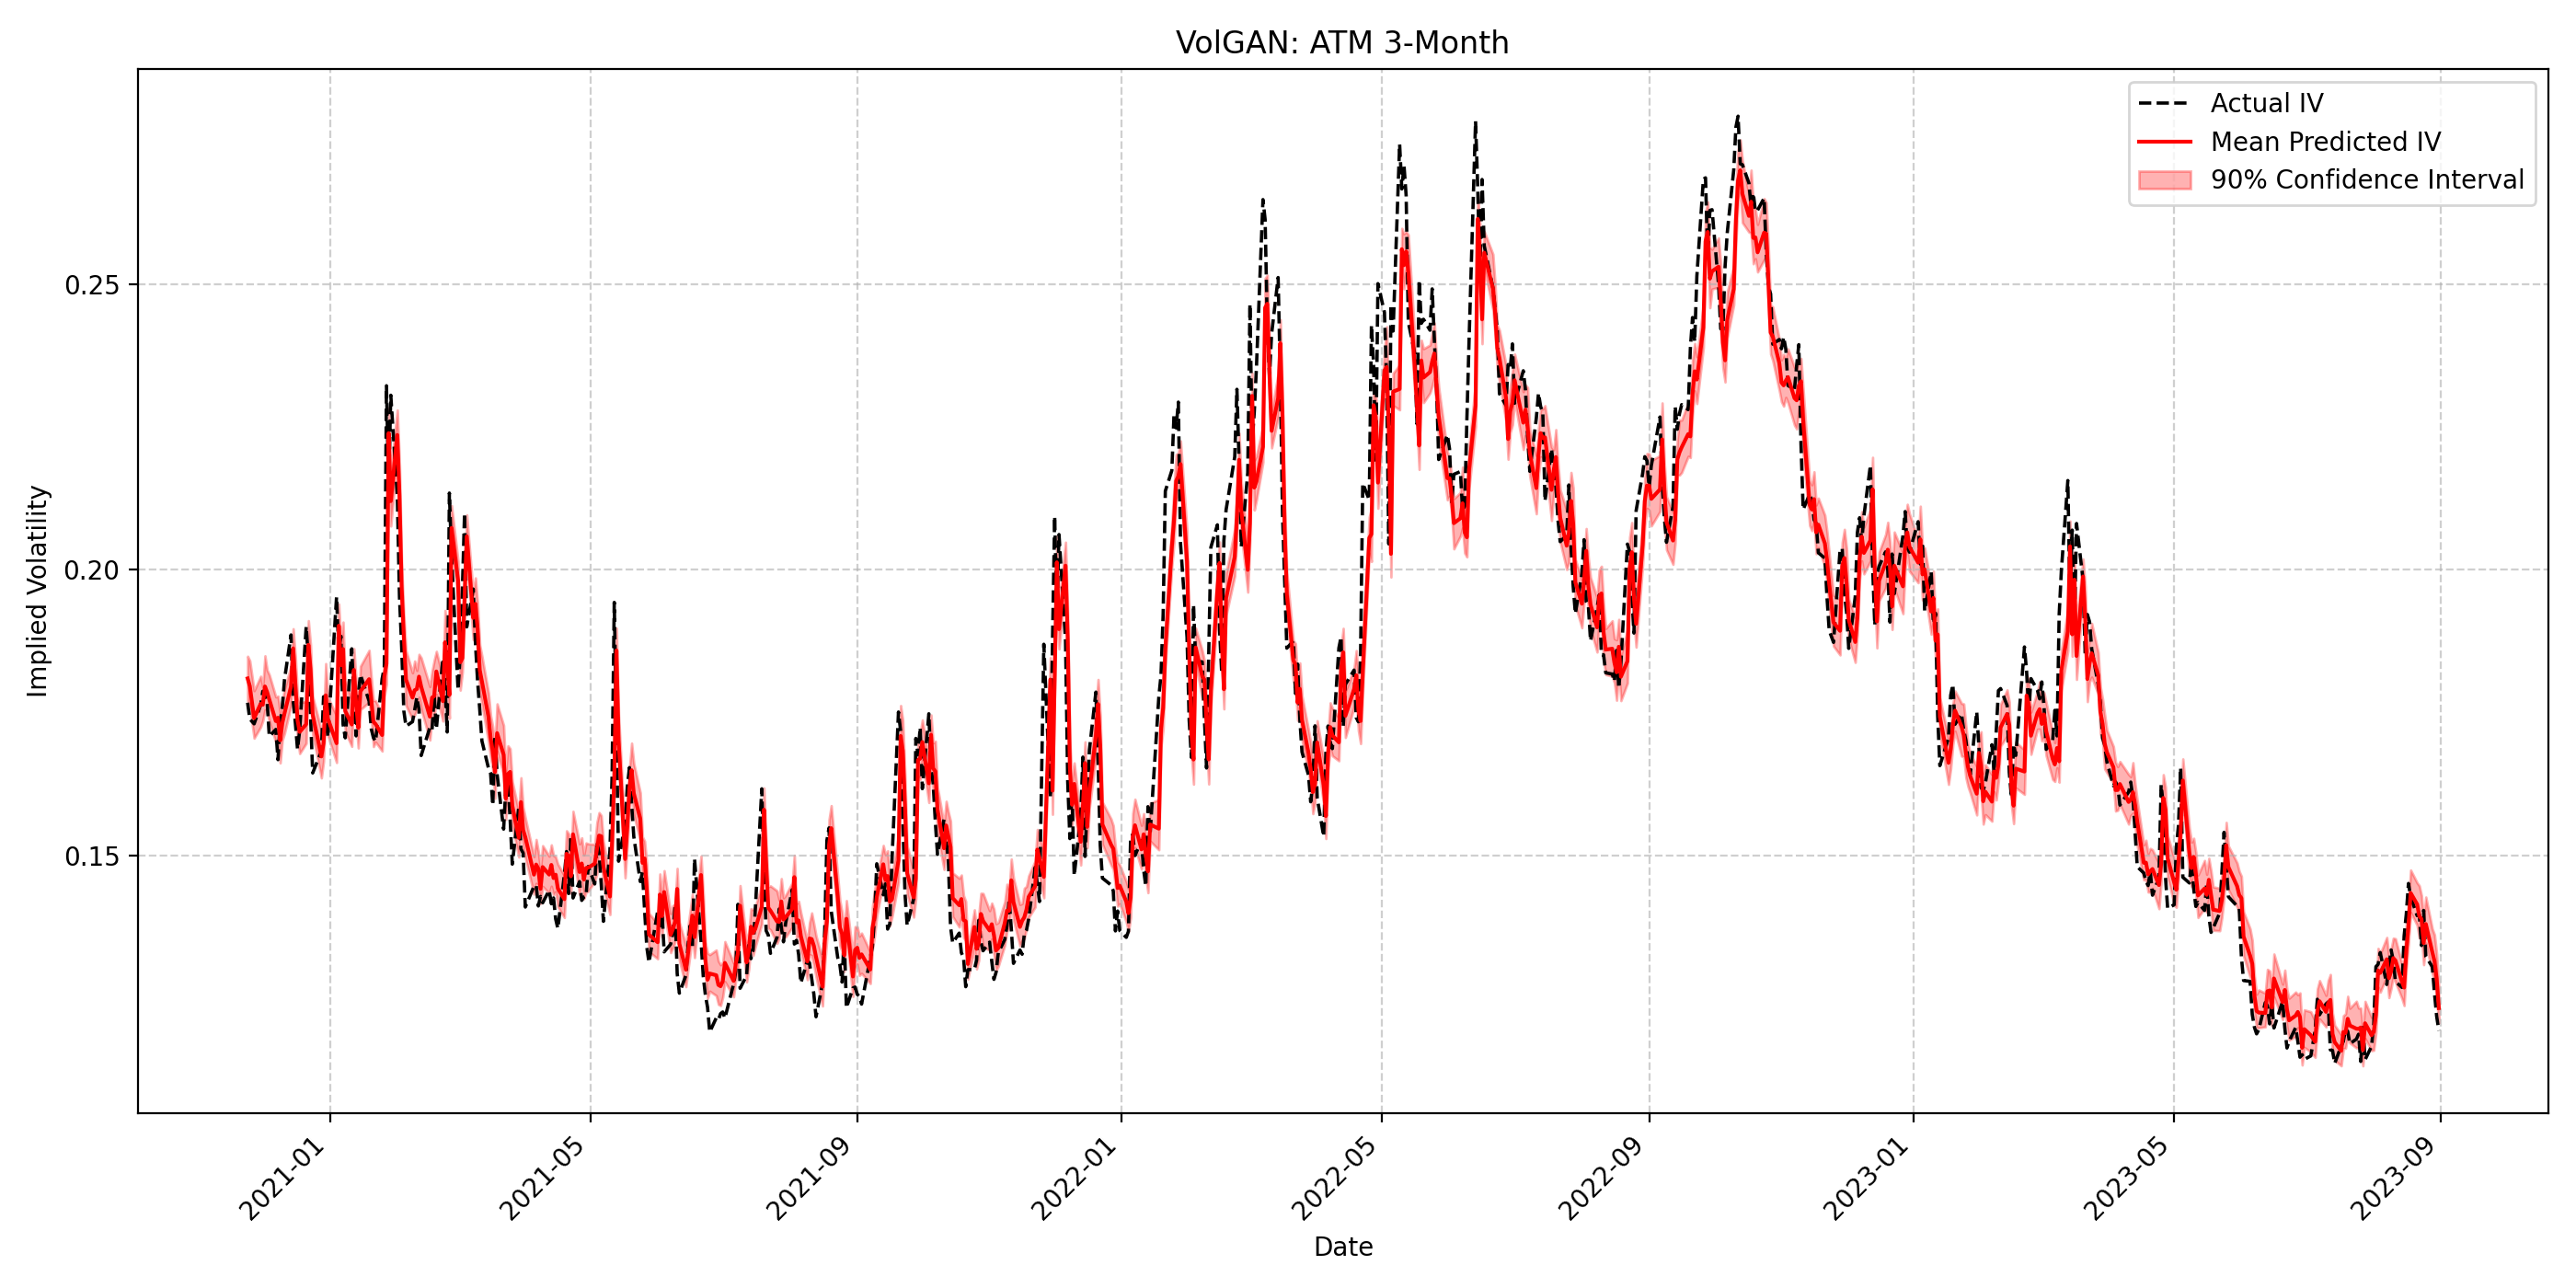
\includegraphics[width=\textwidth]{ts_slice/volgan_atm_3-month_ci.png}
        \caption{VolGAN Model (ATM 3-Month).}
    \end{subfigure}
\end{figure}

% --- FIGURE 2: ITM SLICES ---
\begin{figure}[h!]
    \centering
    \caption{Time series comparison for In-the-Money (ITM) slices. Left: Diffusion Model vs. Real. Right: VolGAN vs. Real.}
    \label{fig:itm_slices}
    
    % --- ITM 1-Month ---
    \begin{subfigure}[b]{0.49\textwidth}
        \centering
        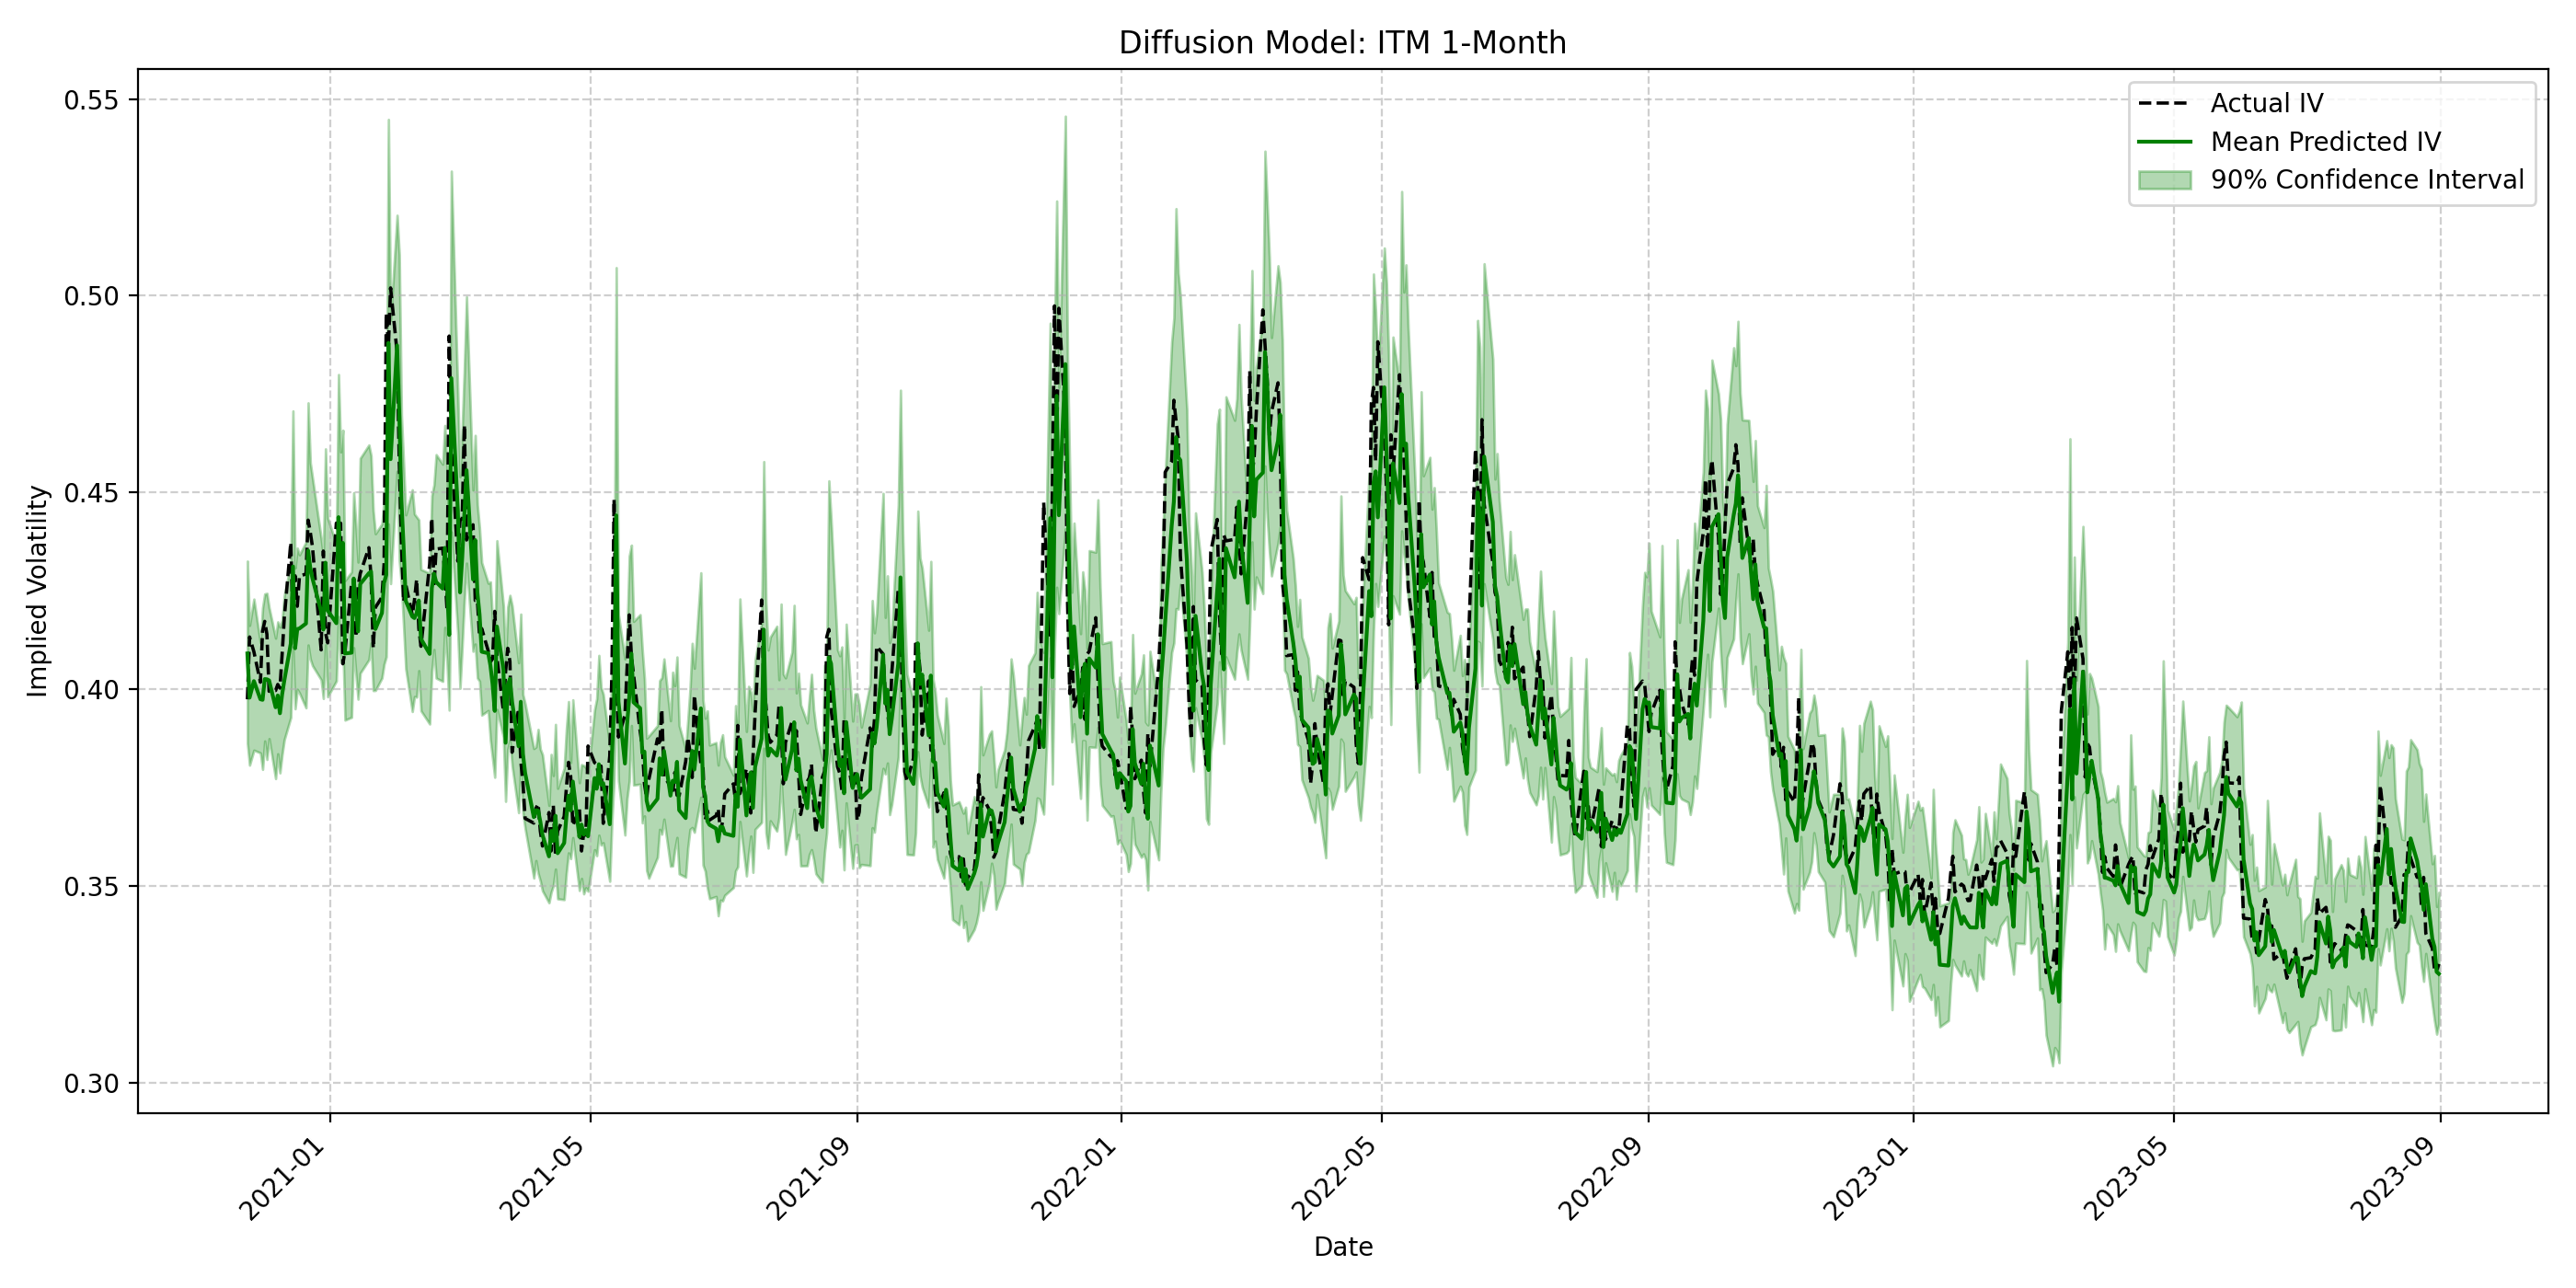
\includegraphics[width=\textwidth]{ts_slice/DiffusionModel_ITM_1-Month_comparison.png}
        \caption{Diffusion Model (ITM 1-Month).}
    \end{subfigure}
    \hfill
    \begin{subfigure}[b]{0.49\textwidth}
        \centering
        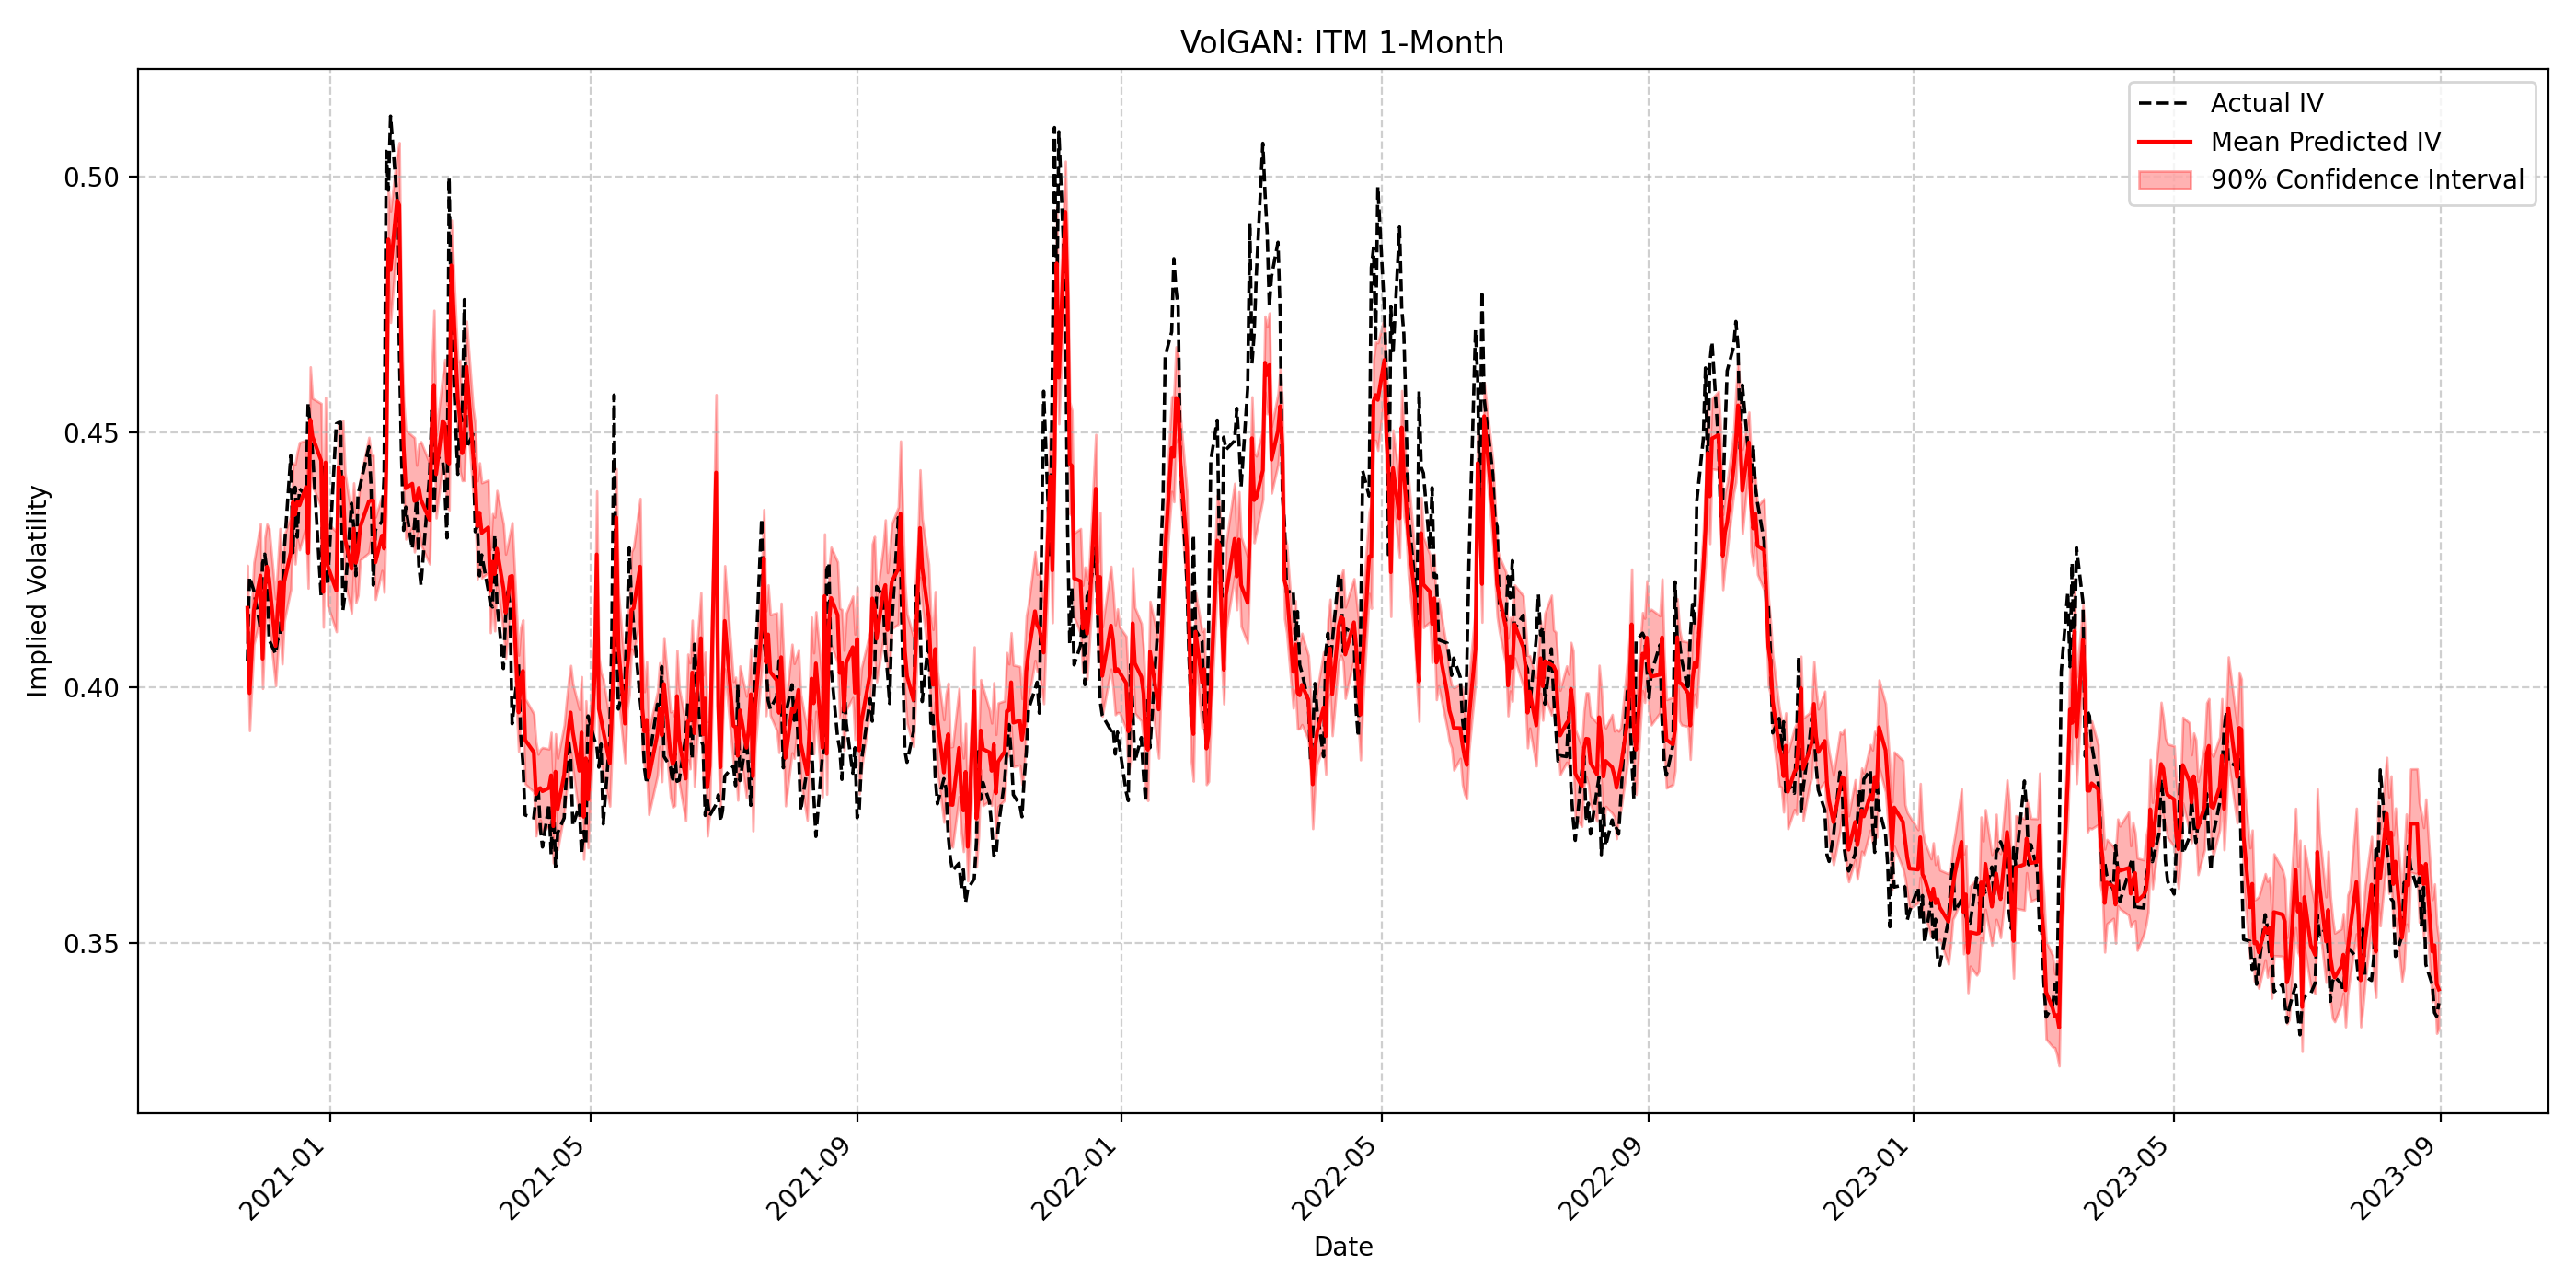
\includegraphics[width=\textwidth]{ts_slice/volgan_itm_1-month_ci.png}
        \caption{VolGAN Model (ITM 1-Month).}
    \end{subfigure}
    
    \vspace{0.5cm}
    
    % --- ITM 3-Month ---
    \begin{subfigure}[b]{0.49\textwidth}
        \centering
        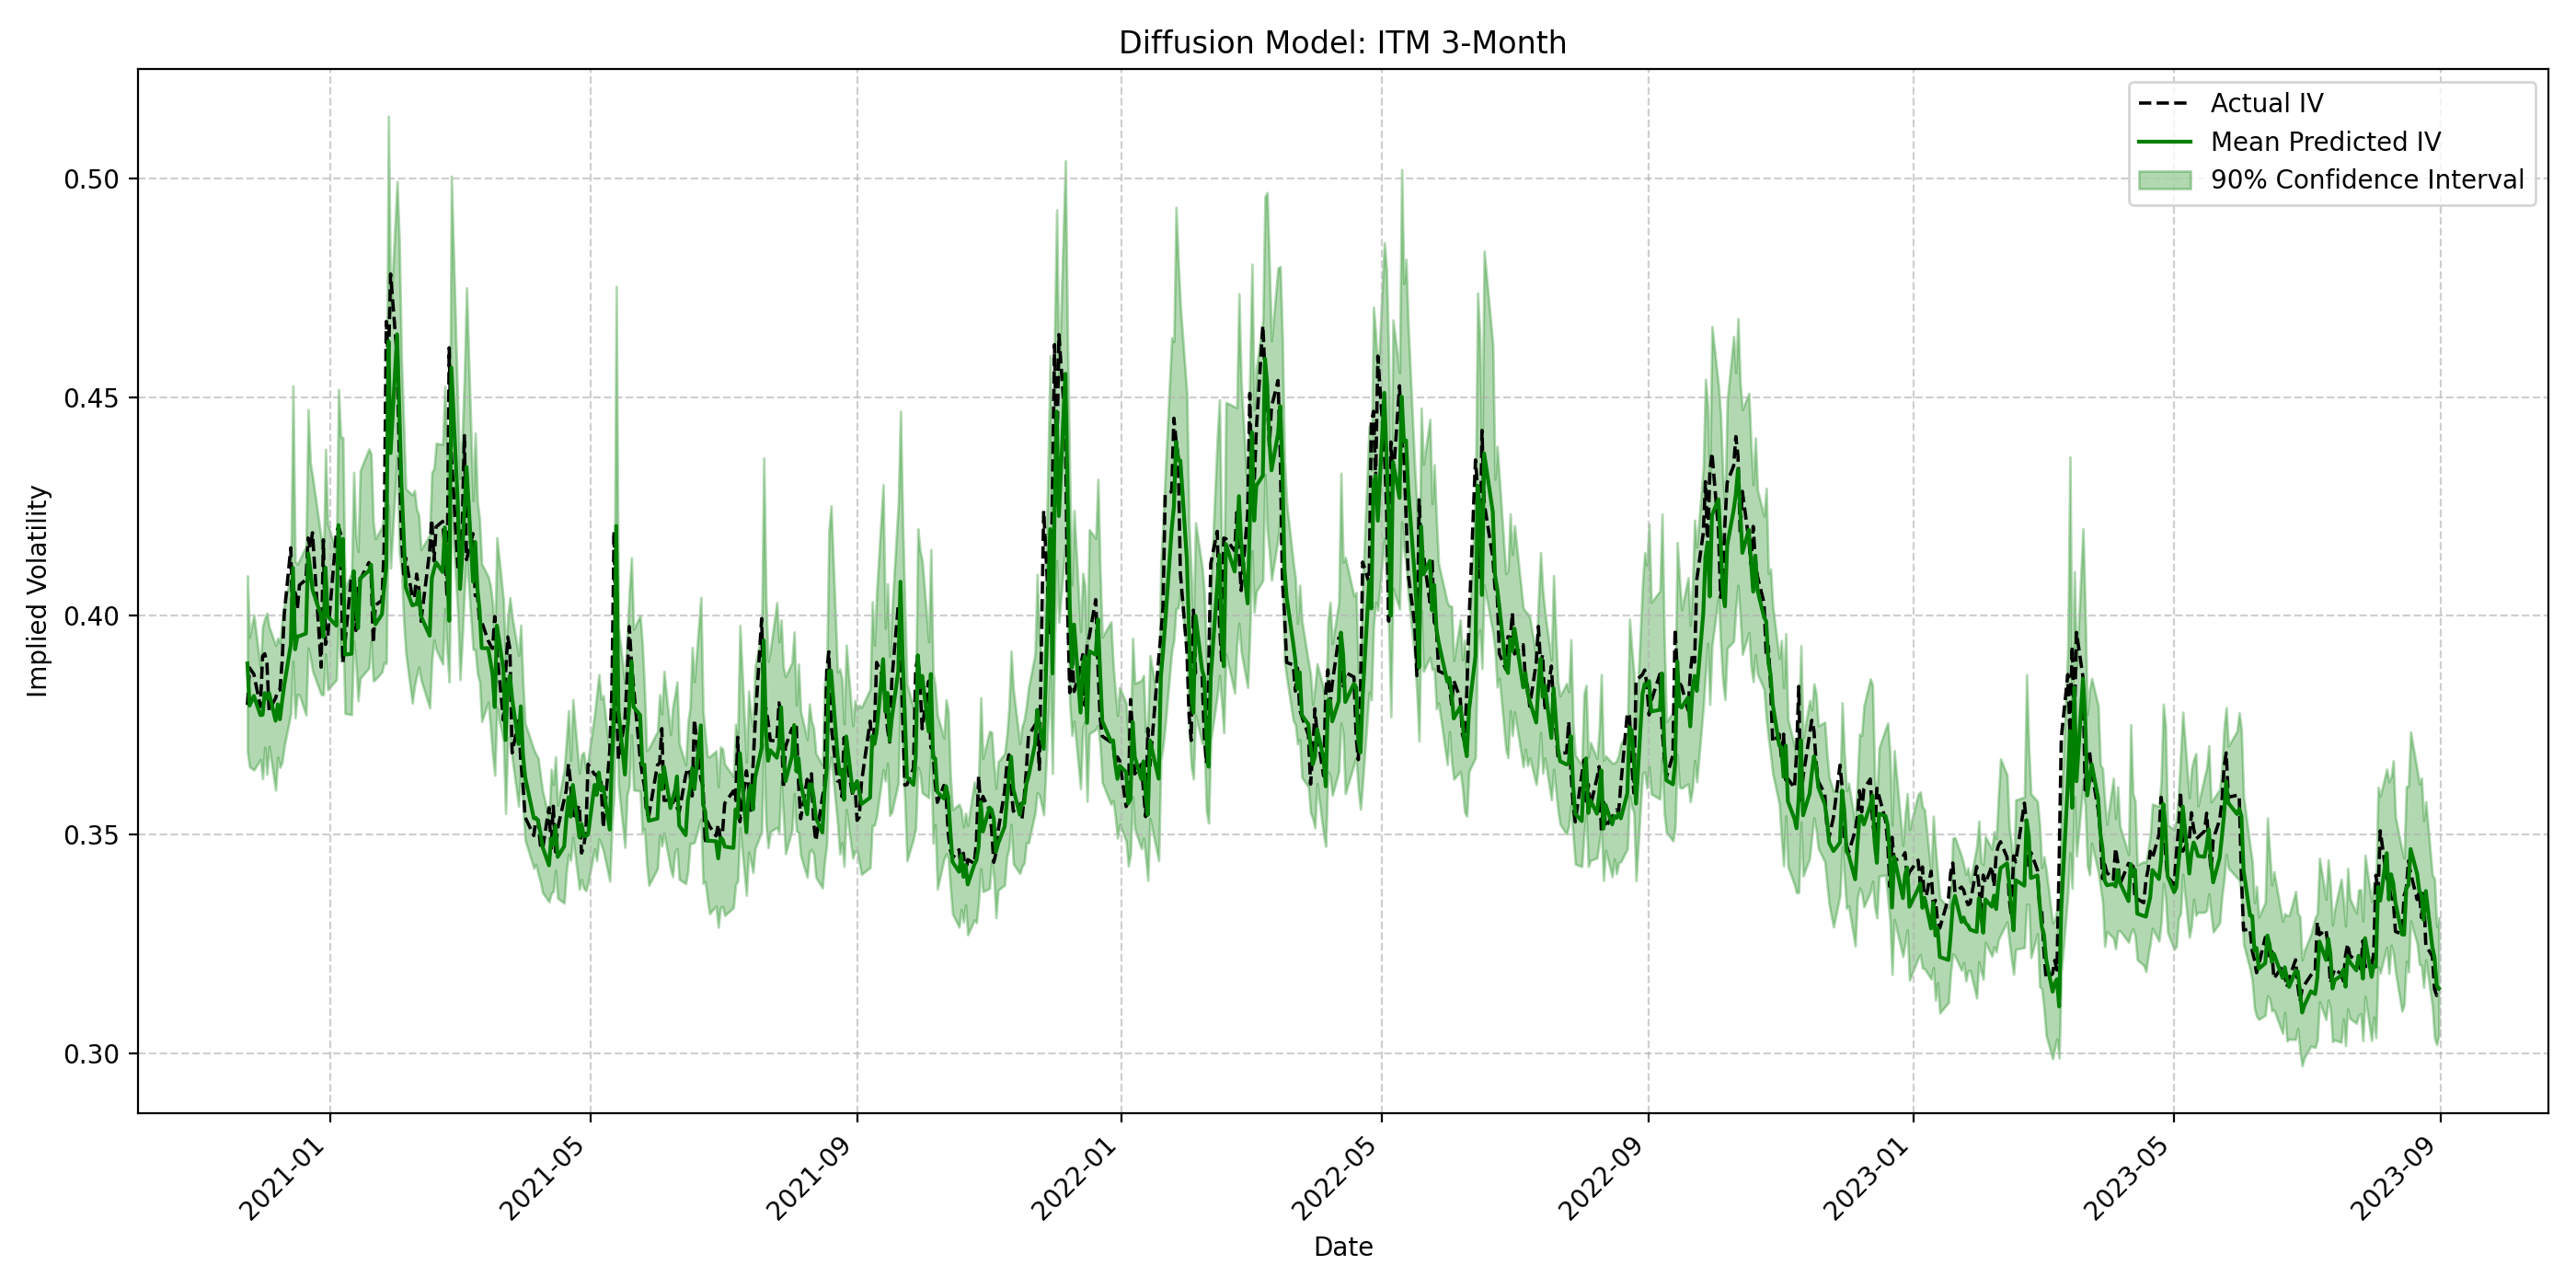
\includegraphics[width=\textwidth]{ts_slice/DiffusionModel_ITM_3-Month_comparison.png}
        \caption{Diffusion Model (ITM 3-Month).}
    \end{subfigure}
    \hfill
    \begin{subfigure}[b]{0.49\textwidth}
        \centering
        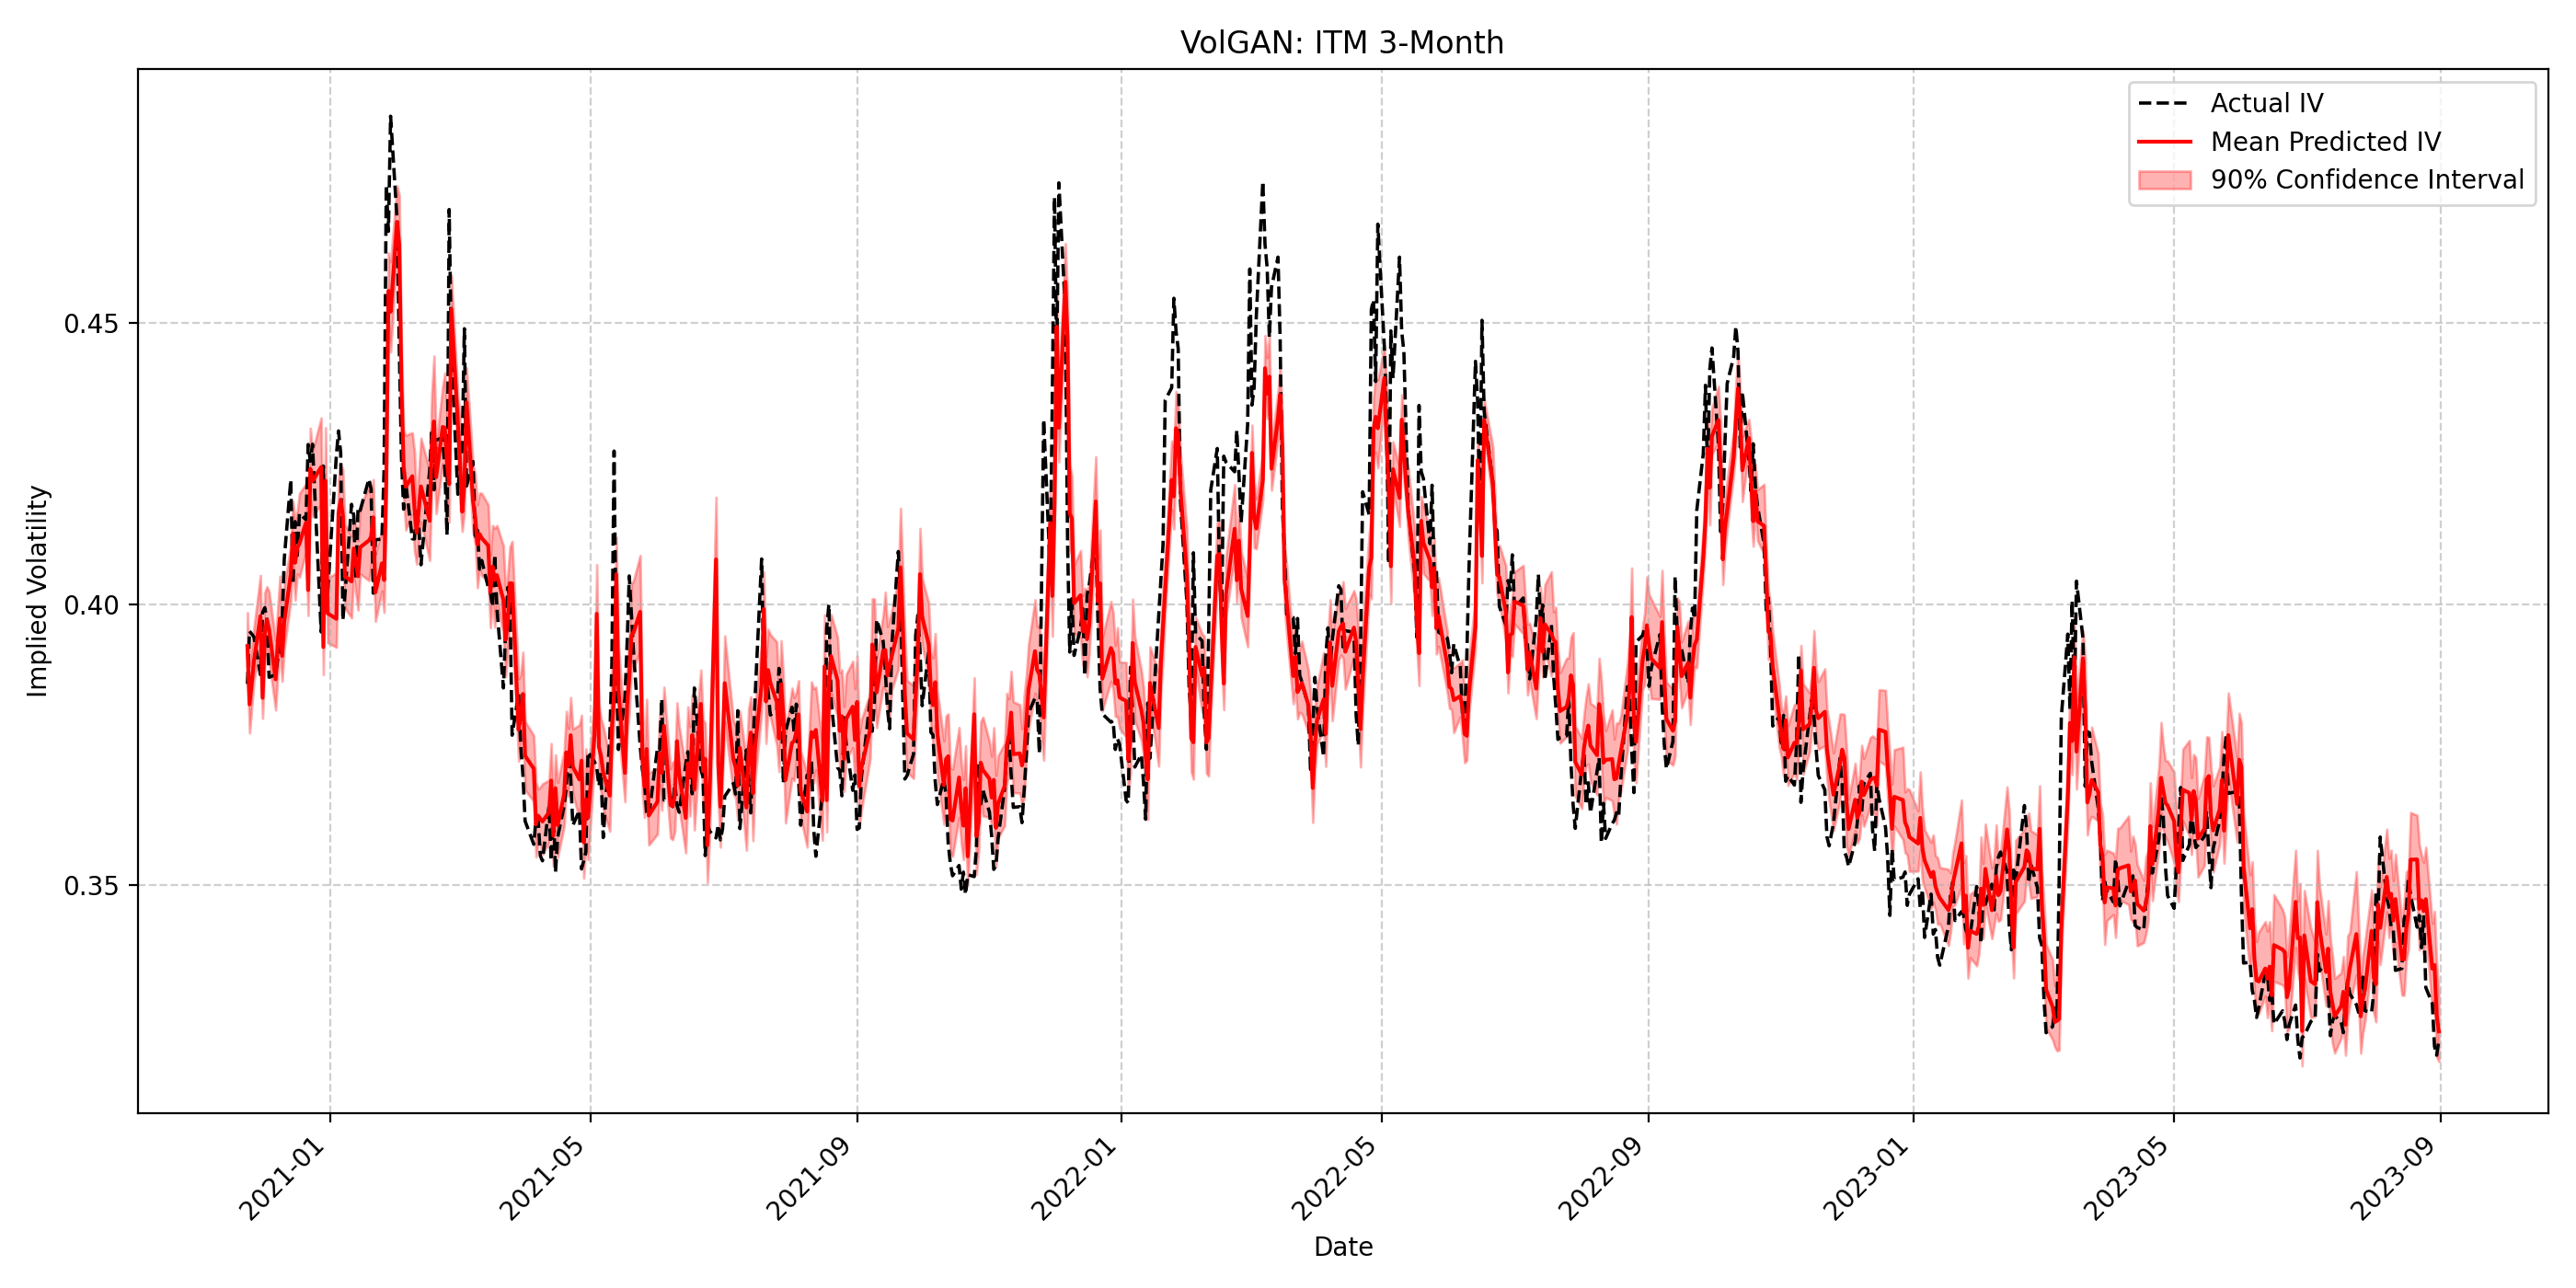
\includegraphics[width=\textwidth]{ts_slice/volgan_itm_3-month_ci.png}
        \caption{VolGAN Model (ITM 3-Month).}
    \end{subfigure}
\end{figure}

% --- FIGURE 3: OTM SLICES ---
\begin{figure}[h!]
    \centering
    \caption{Time series comparison for Out-of-the-Money (OTM) slices. Left: Diffusion Model vs. Real. Right: VolGAN vs. Real.}
    \label{fig:otm_slices}
    
    % --- OTM 1-Month ---
    \begin{subfigure}[b]{0.49\textwidth}
        \centering
        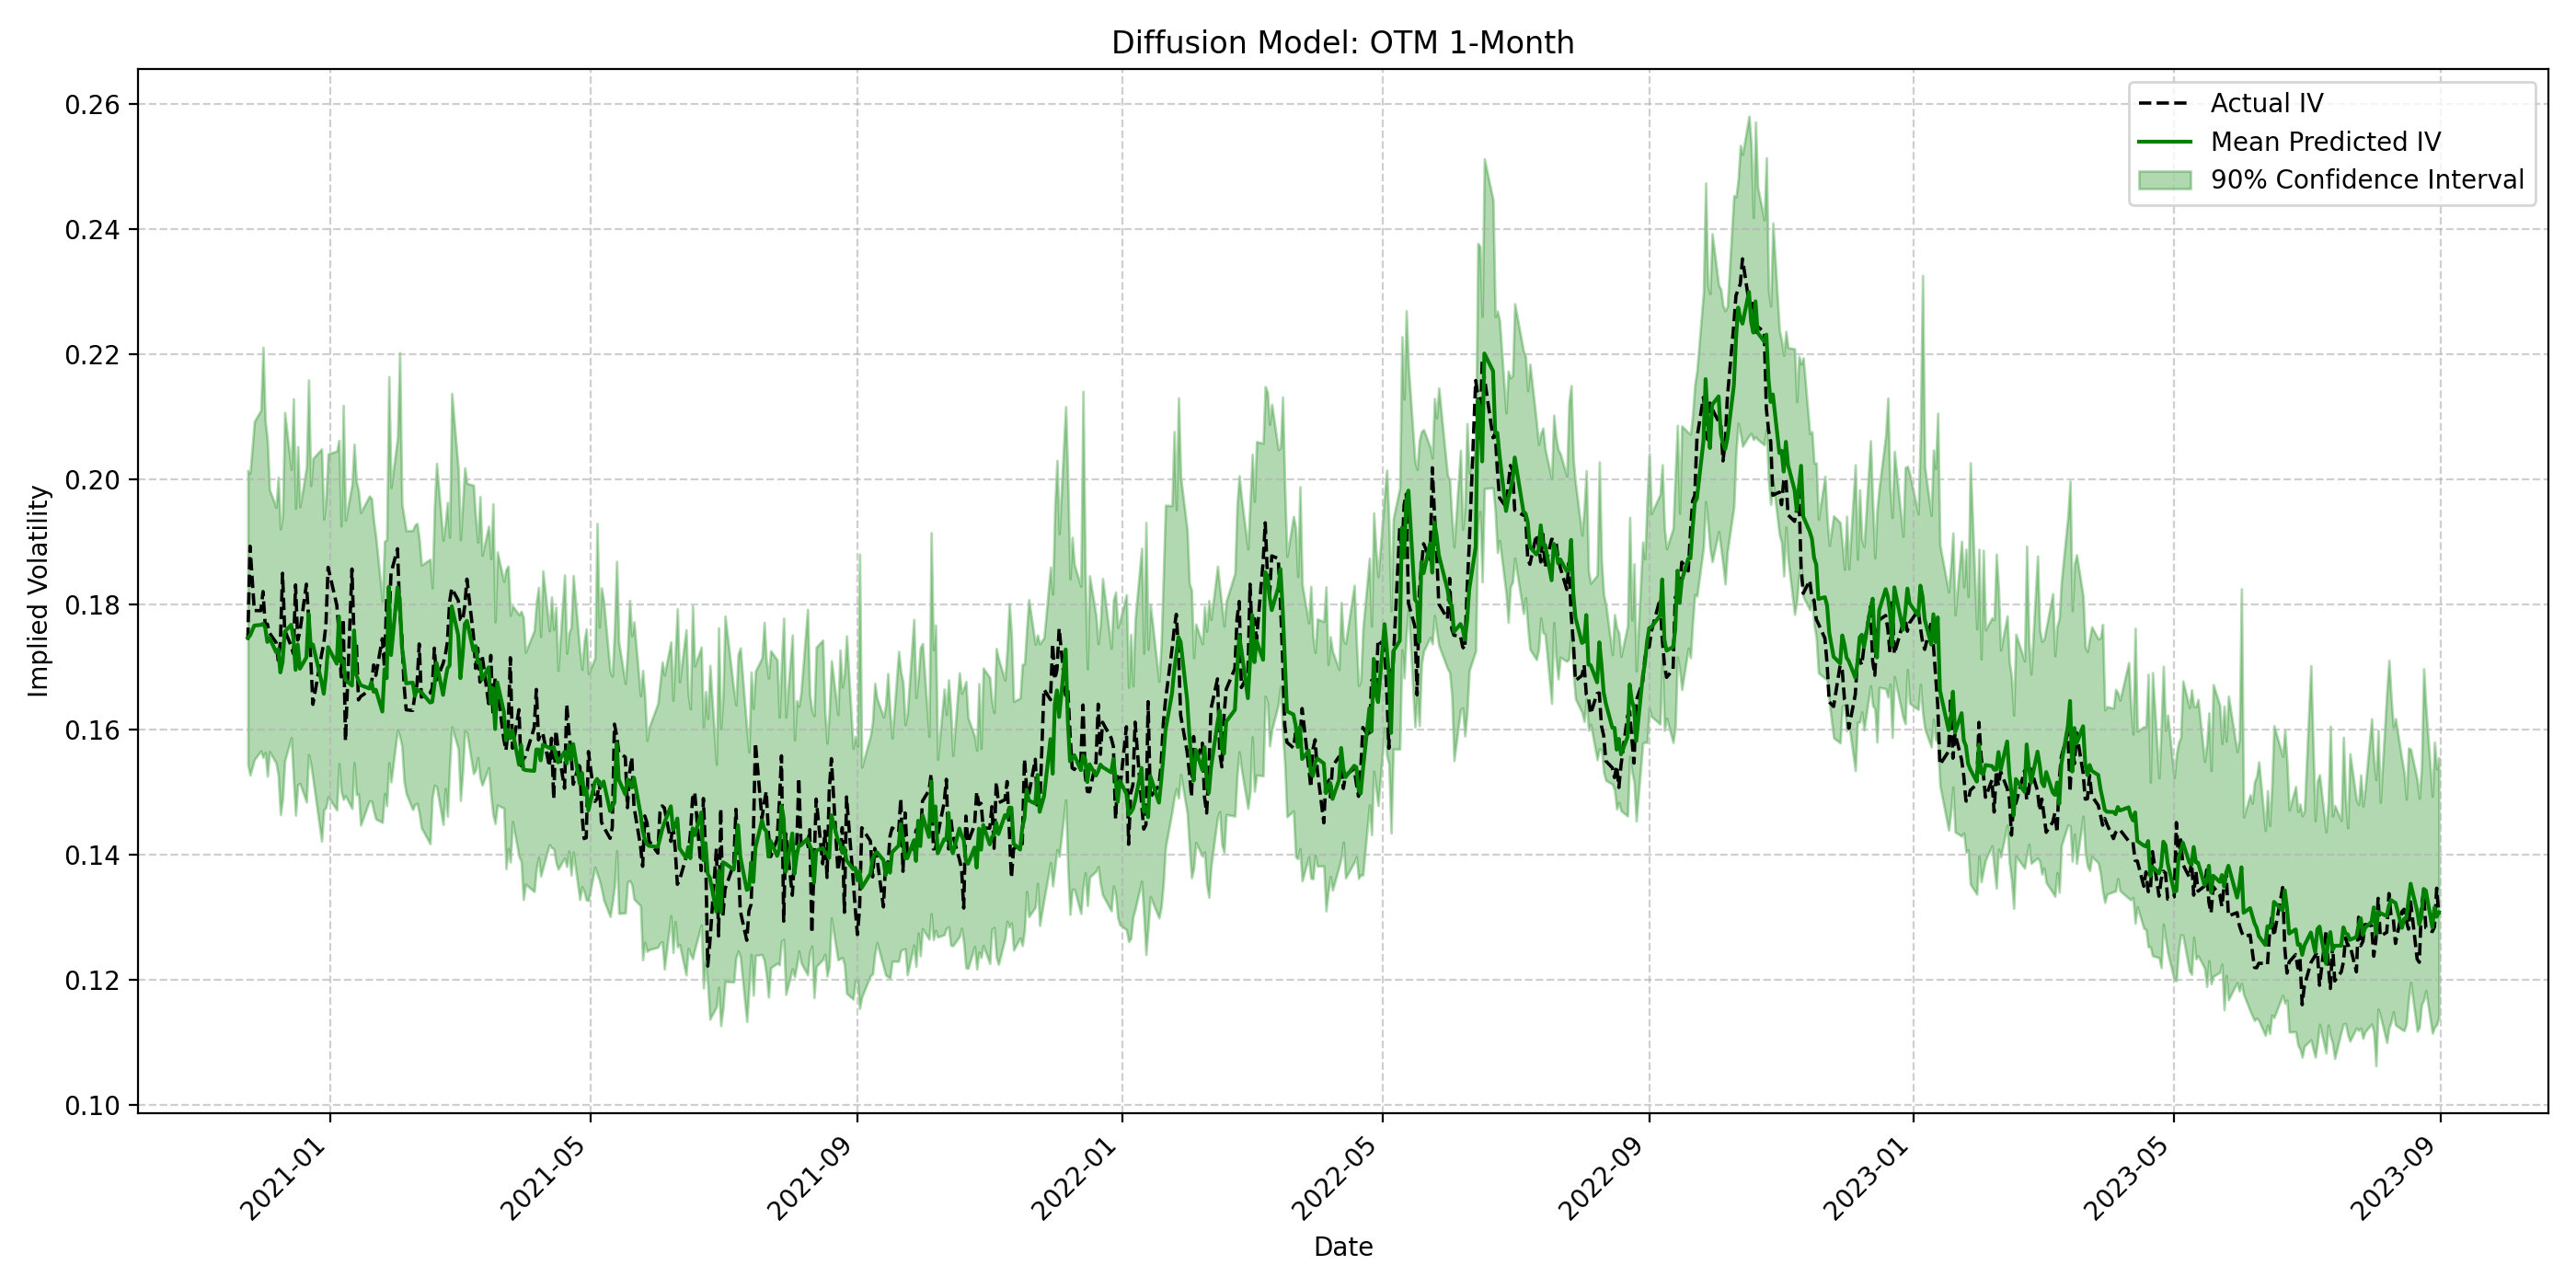
\includegraphics[width=\textwidth]{ts_slice/DiffusionModel_OTM_1-Month_comparison.png}
        \caption{Diffusion Model (OTM 1-Month).}
    \end{subfigure}
    \hfill
    \begin{subfigure}[b]{0.49\textwidth}
        \centering
        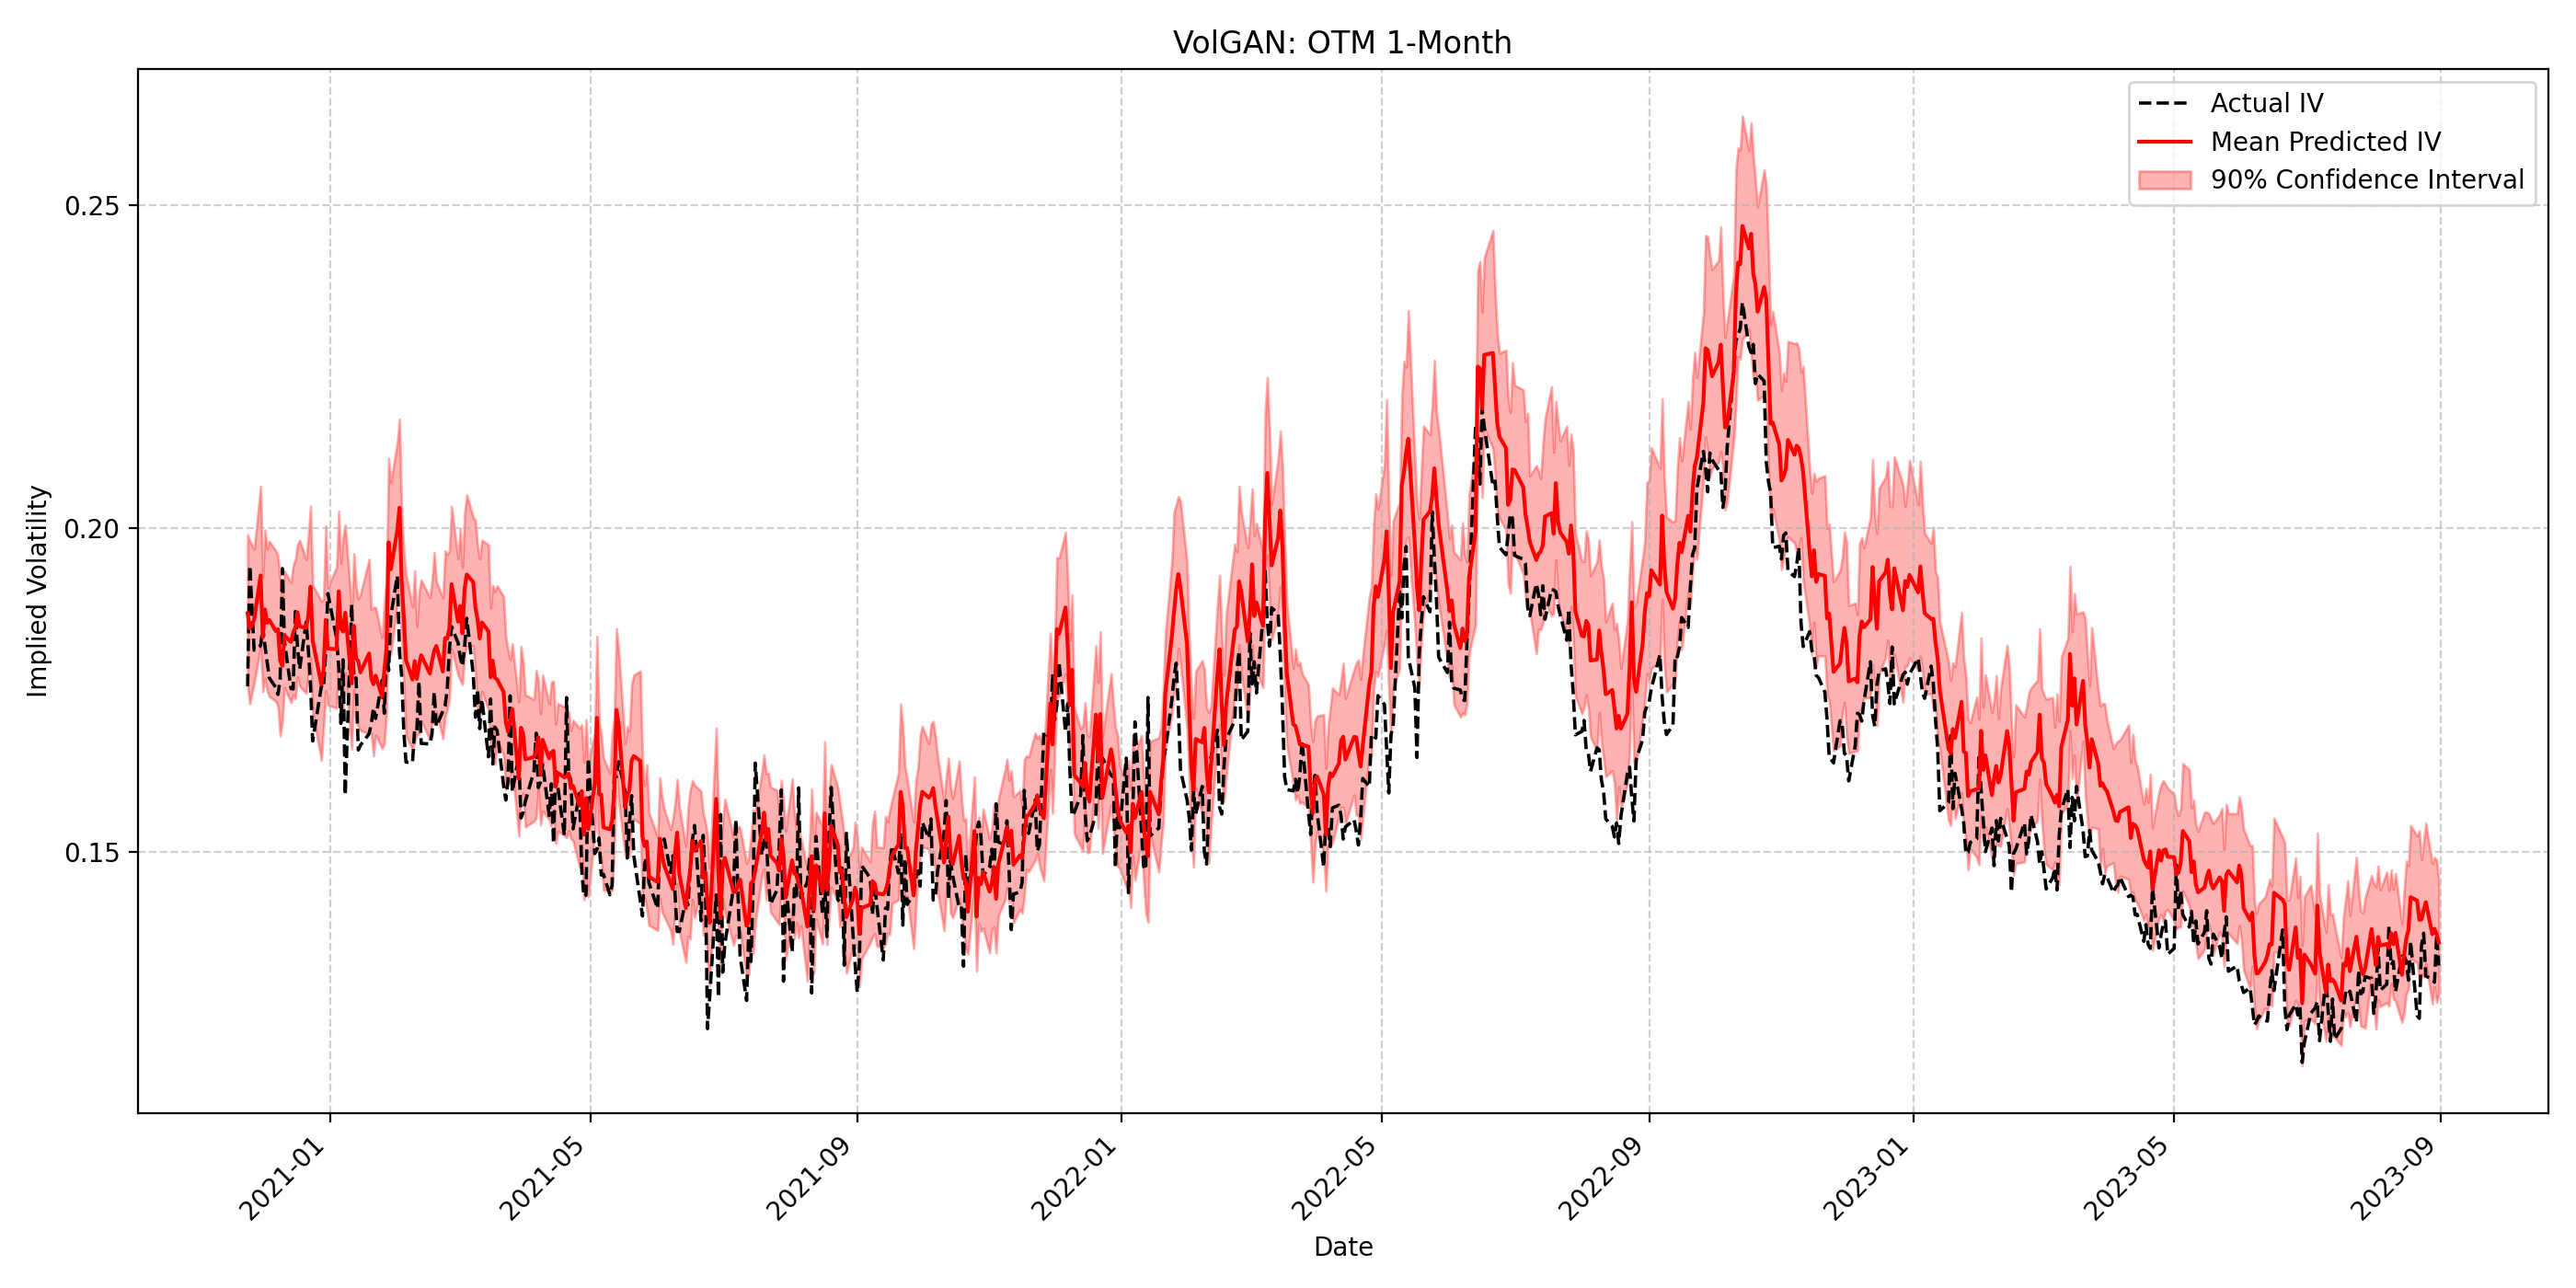
\includegraphics[width=\textwidth]{ts_slice/volgan_otm_1-month_ci.png}
        \caption{VolGAN Model (OTM 1-Month).}
    \end{subfigure}
    
    \vspace{0.5cm}

    % --- OTM 3-Month ---
    \begin{subfigure}[b]{0.49\textwidth}
        \centering
        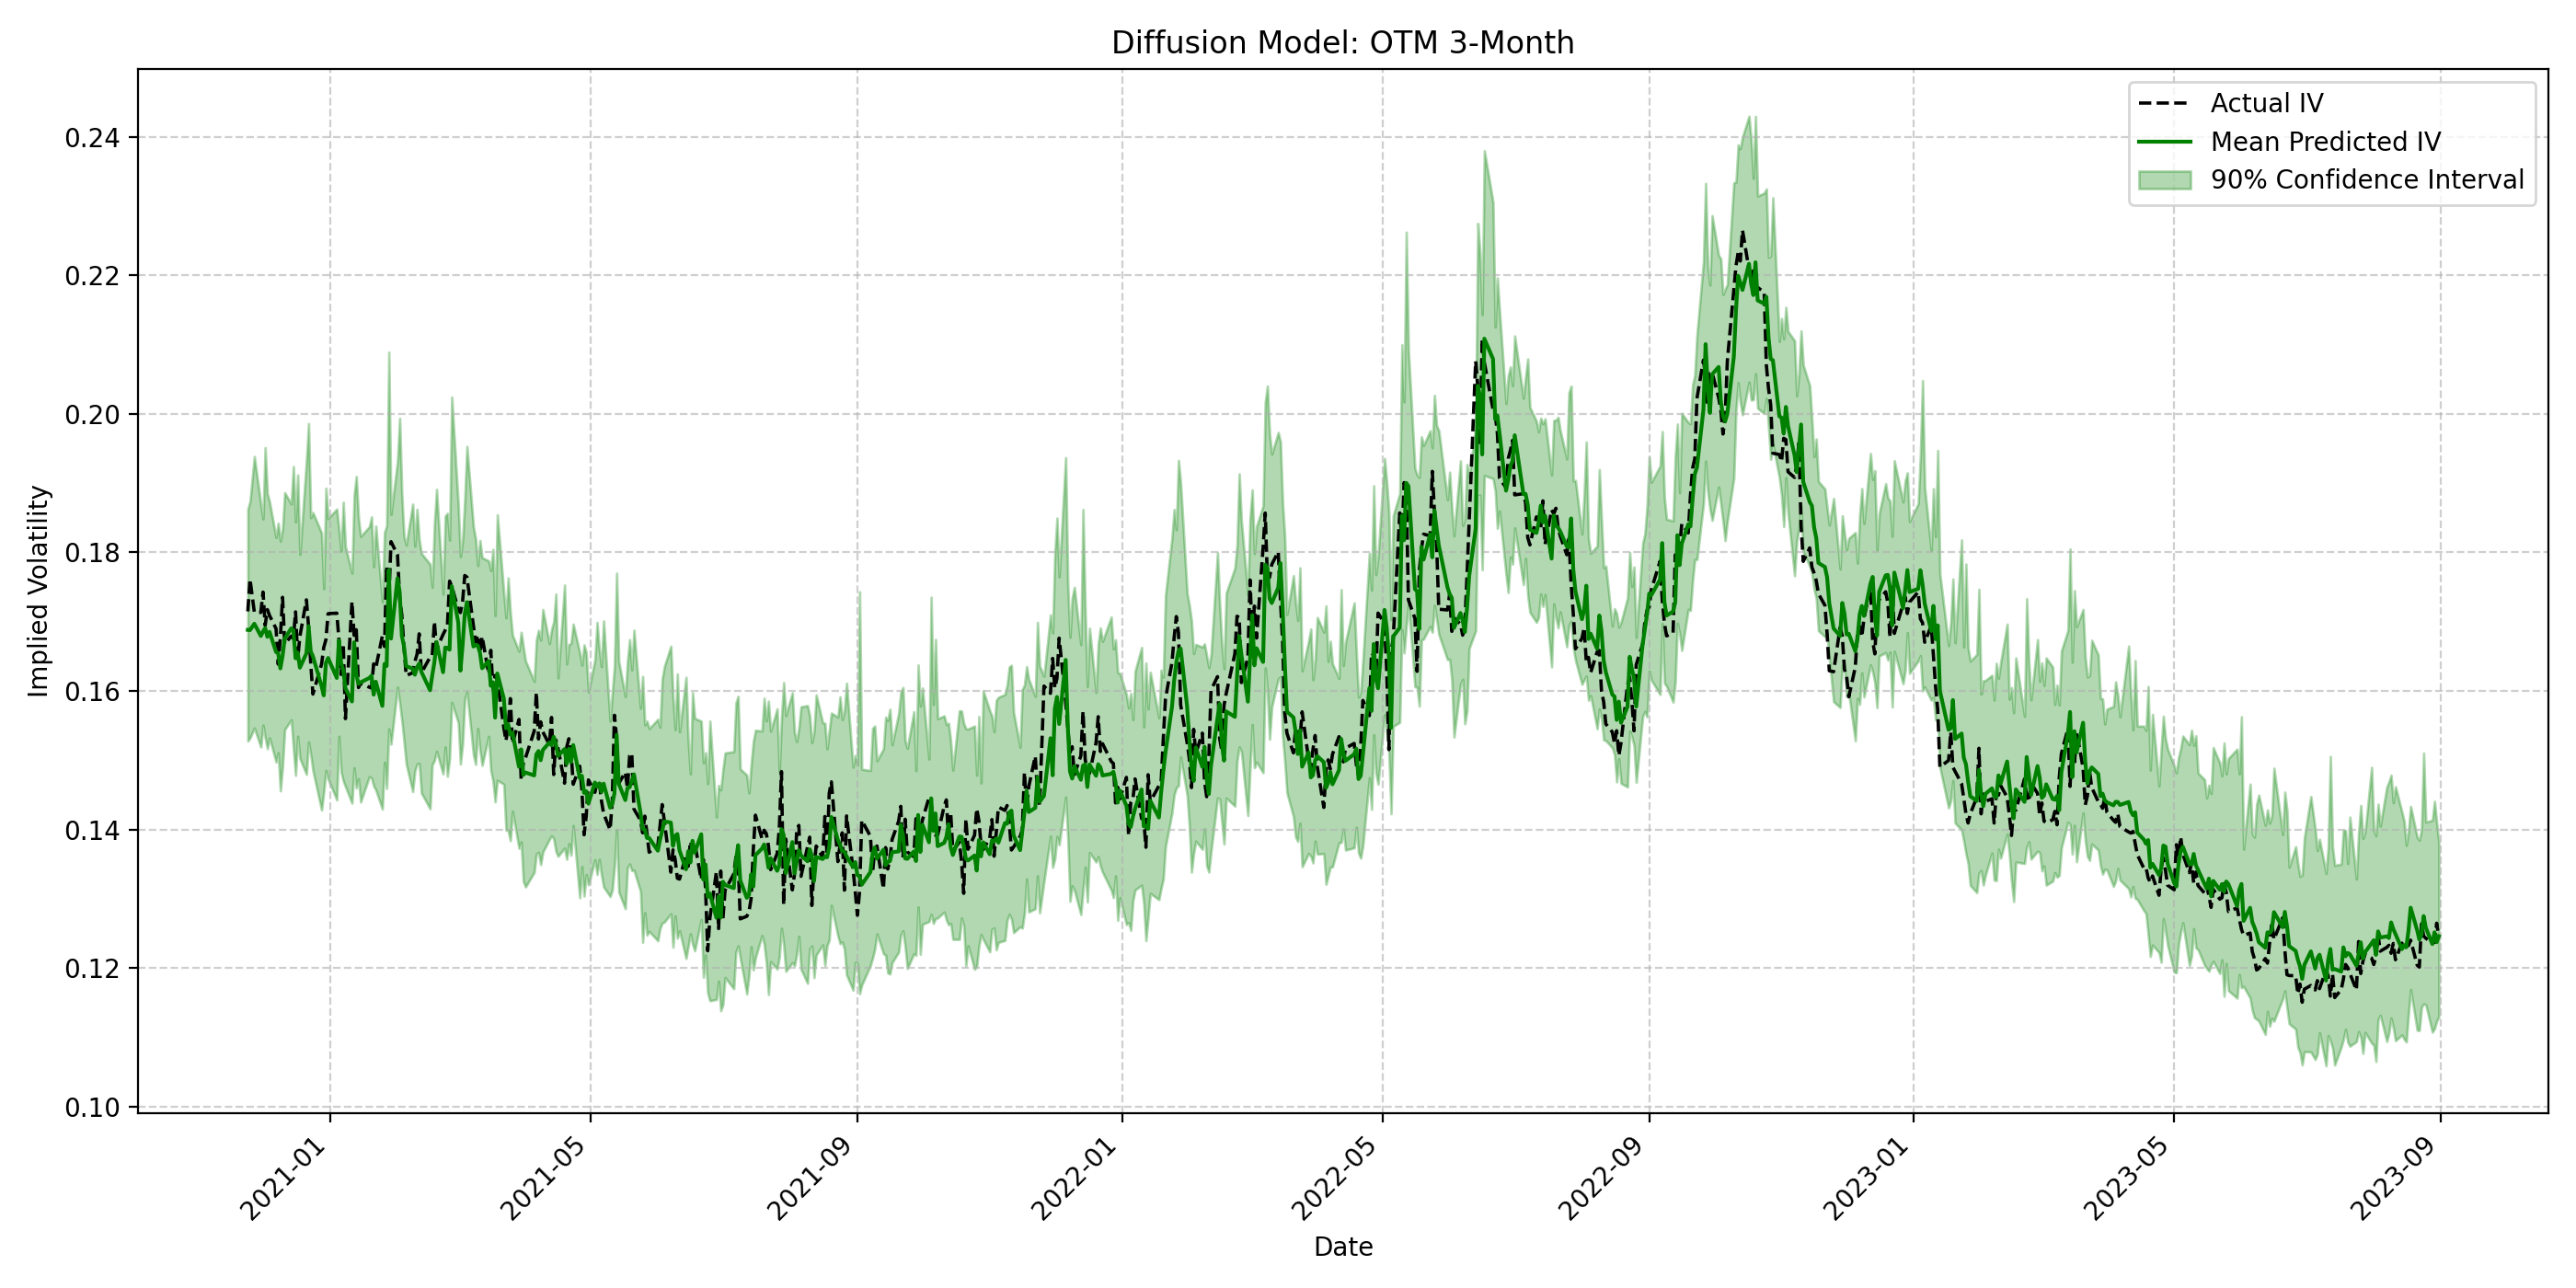
\includegraphics[width=\textwidth]{ts_slice/DiffusionModel_OTM_3-Month_comparison.png}
        \caption{Diffusion Model (OTM 3-Month).}
    \end{subfigure}
    \hfill
    \begin{subfigure}[b]{0.49\textwidth}
        \centering
        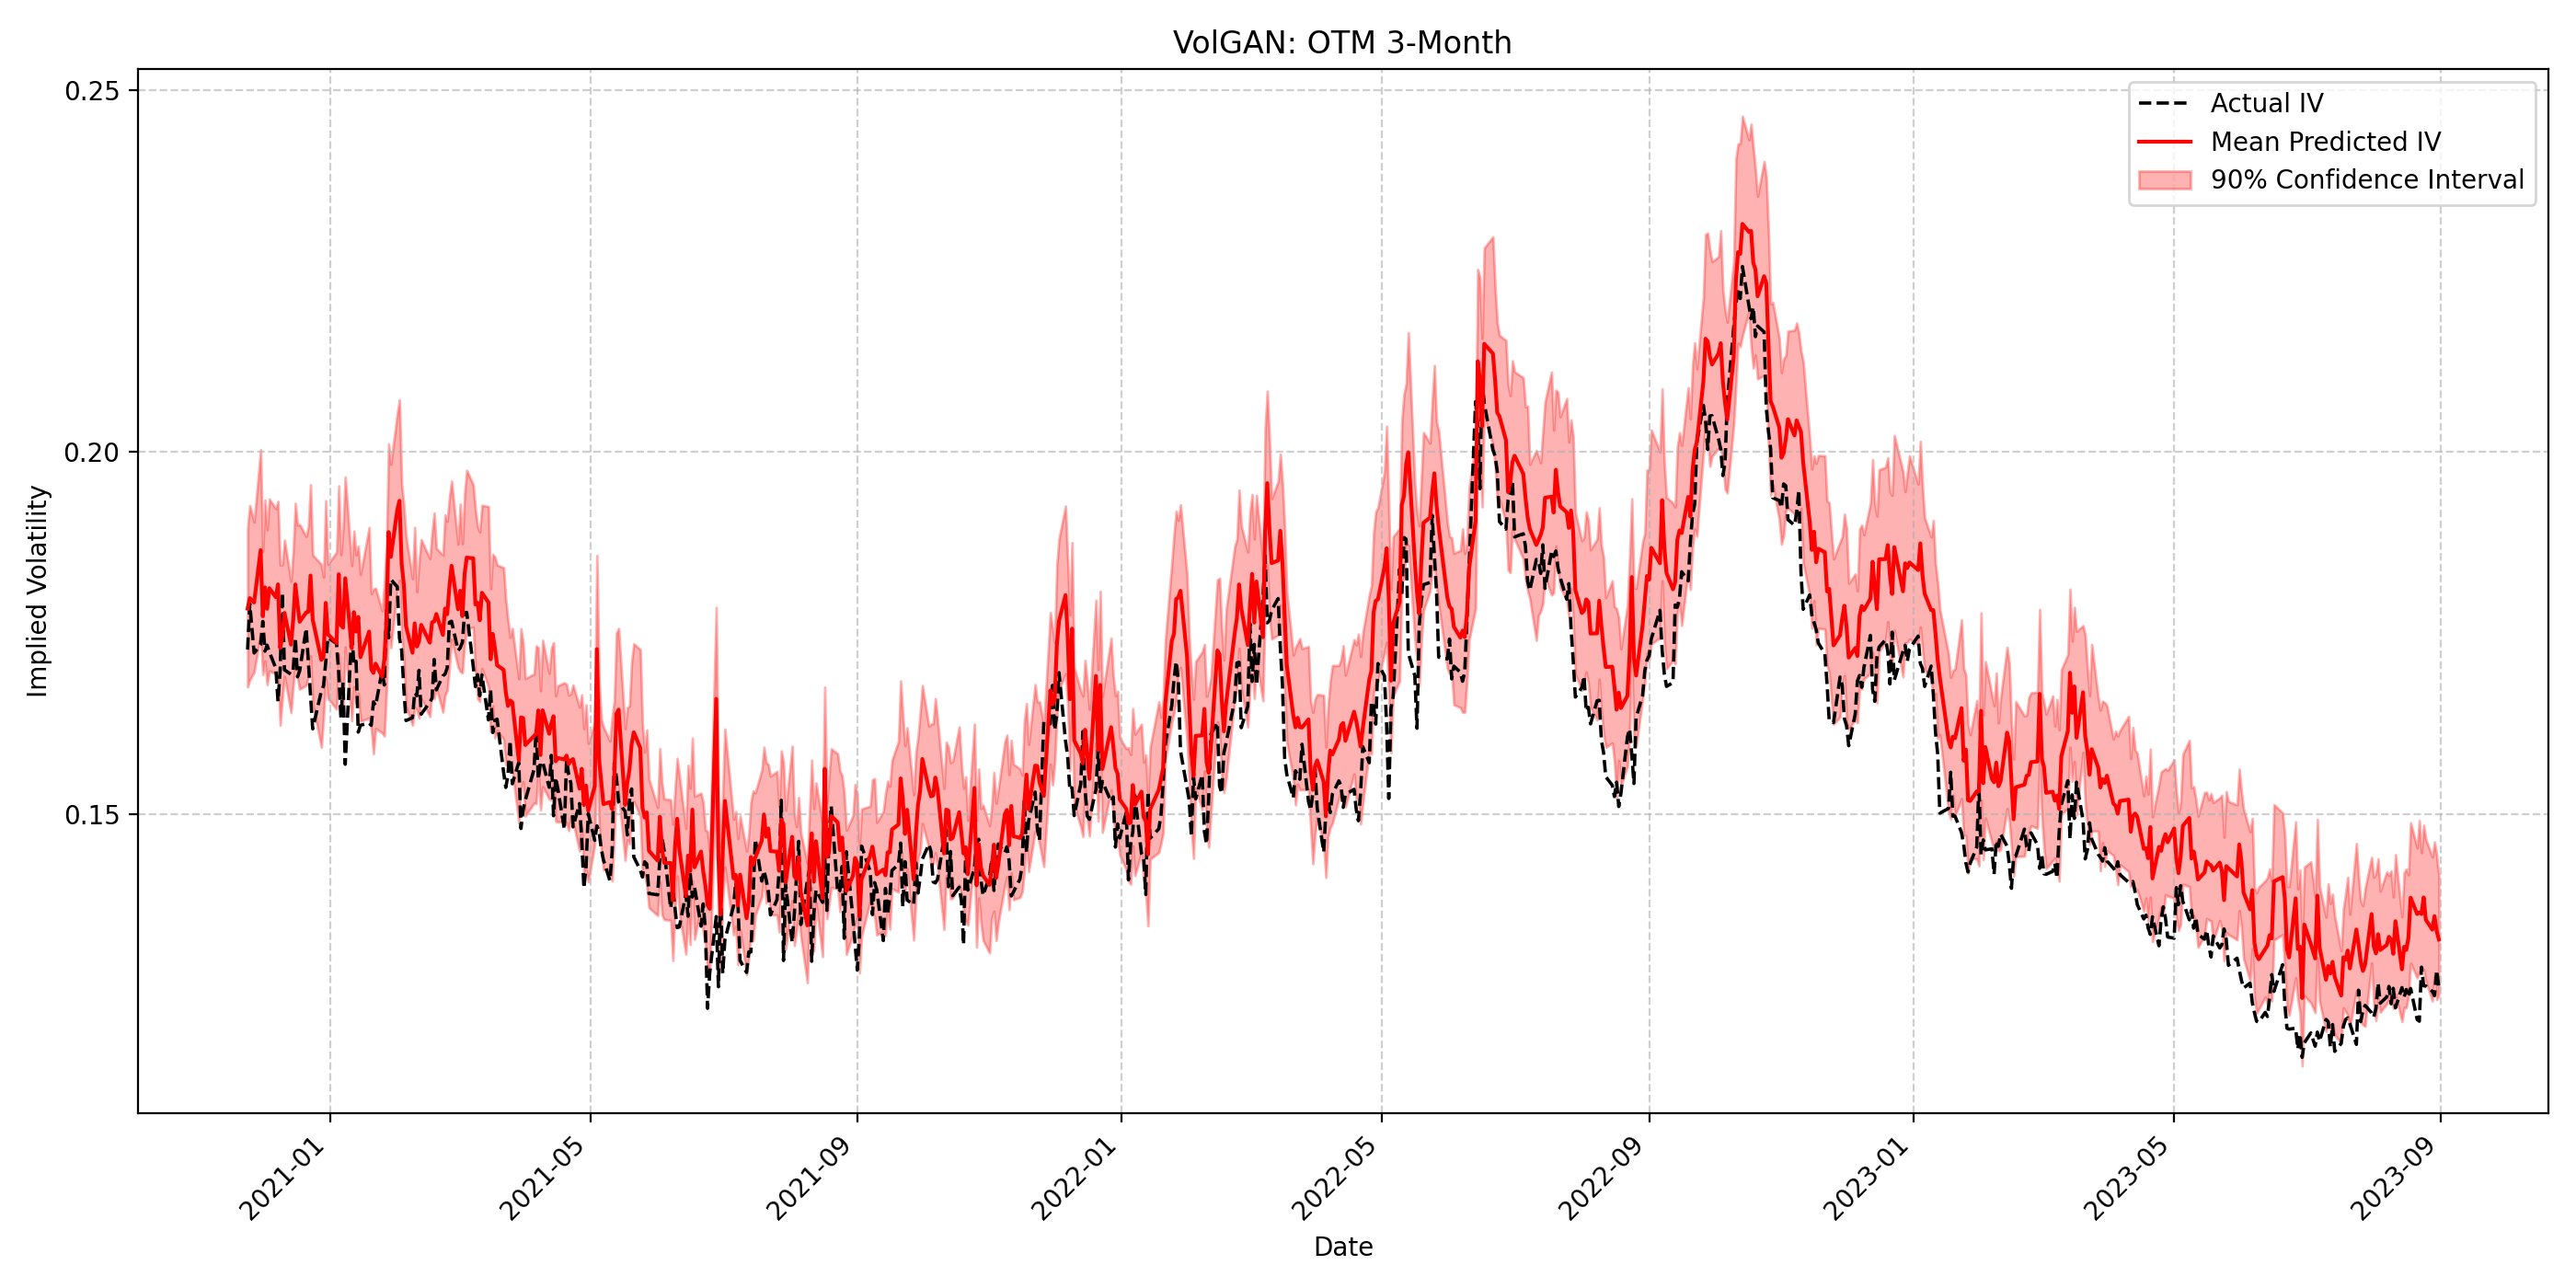
\includegraphics[width=\textwidth]{ts_slice/volgan_otm_3-month_ci.png}
        \caption{VolGAN Model (OTM 3-Month).}
    \end{subfigure}
\end{figure}

\begin{table}[h!]
\centering
\caption{Comparison of Model Performance Metrics.}
\label{tab:performance_metrics}
\resizebox{\textwidth}{!}{%
\begin{tabular}{l rrrrrrrrrrrrr}
\toprule
% --- Hierarchical Column Headers ---
& \multicolumn{4}{c}{ATM} & \multicolumn{4}{c}{OTM} & \multicolumn{4}{c}{ITM} & \\
\cmidrule(lr){2-5} \cmidrule(lr){6-9} \cmidrule(lr){10-13}
% --- Sub-Headers ---
Metric & 1-Day & 1-Week & 1-Month & 3-Month & 1-Day & 1-Week & 1-Month & 3-Month & 1-Day & 1-Week & 1-Month & 3-Month & Overall \\
\midrule

% --- VolGAN 5 Data ---
\multicolumn{14}{l}{\textbf{VolGAN}} \\
MAPE (\%) & 4.8882 & 4.8595 & 4.6231 & 4.2498 & 5.5066 & 5.7265 & 5.0659 & 4.0762 & 2.9814 & 2.9420 & 2.6978 & 2.3652 & 3.7304 \\
Std. of APE (\%) & 4.0258 & 4.0304 & 3.9043 & 3.5292 & 4.8518 & 4.9798 & 4.3324 & 3.5471 & 2.4231 & 2.4151 & 2.2283 & 1.8661 &  \\
Mean CI Width & 0.0158 & 0.0159 & 0.0146 & 0.0151 & 0.0726 & 0.0679 & 0.0654 & 0.0474 & 0.0347 & 0.0292 & 0.0248 & 0.0128 &  \\
Std. CI Width & 0.0073 & 0.0072 & 0.0064 & 0.0047 & 0.0172 & 0.0149 & 0.0141 & 0.0099 & 0.0091 & 0.0075 & 0.0055 & 0.0023 &  \\
CI Breach \% & 44.8276 & 43.8218 & 45.6897 & 40.5172 & 1.5805 & 2.5862 & 1.0057 & 1.0057 & 31.4655 & 35.0575 & 36.7816 & 57.1839 &  \\
\addlinespace

% --- Diffusion Data ---
\multicolumn{14}{l}{\textbf{Diffusion}} \\
MAPE (\%) & 4.6907 & 4.6884 & 4.5146 & 4.0202 & 3.5264 & 3.4573 & 3.1542 & 2.4555 & 2.5129 & 2.4992 & 2.4184 & 2.2024 & 3.0026 \\
Std. of APE (\%) & 4.0338 & 4.0091 & 3.8795 & 3.4909 & 2.6588 & 2.5785 & 2.3190 & 1.8739 & 2.3984 & 2.3844 & 2.2909 & 2.0393 &  \\
Mean CI Width & 0.0372 & 0.0369 & 0.0357 & 0.0327 & 0.0468 & 0.0457 & 0.0412 & 0.0311 & 0.0472 & 0.0463 & 0.0438 & 0.0384 &  \\
Std. CI Width & 0.0160 & 0.0159 & 0.0152 & 0.0134 & 0.0098 & 0.0095 & 0.0082 & 0.0057 & 0.0139 & 0.0137 & 0.0132 & 0.0124 & \\
CI Breach \% & 10.9195 & 10.4885 & 11.0632 & 10.0575 & 0.5747 & 0.7184 & 0.5747 & 1.0057 & 7.9023 & 7.9023 & 8.4770 & 7.9023 &  \\
\bottomrule
\end{tabular}
}
\end{table}
We trained 9 VolGAN models and selected the best-performing one, based on overall MAPE, as our benchmark for comparison to avoid the instability of GAN. The performance metrics, detailed in Table \ref{tab:performance_metrics}, summarize the performance of our proposed diffusion model. A more detailed table that includes all GAN models is shown in Appendix \ref{sec:appendix_full_table}.
Our diffusion model demonstrates strong predictive accuracy, achieving an Overall MAPE of 3.0026\%, which is lower than the benchmark's 3.7304\%. This indicates a consistent ability to capture the central tendency of the implied volatility surface.
To evaluate the reliability of our uncertainty estimates, we measure the 90\% confidence interval brach (CI Breach \%) rate. This metric calculates the percentage of days in the test set where the ground-truth IV value fell outside the 90\% confidence interval generated by our model (i.e., below the 5th percentile or above the 95th percentile of the 100 generated samples). For a perfectly calibrated model, this breach rate should be around 10\%. Our model's CI Breach \% 
%\aa{(AA: What is this CI breach? Do you define it anywhere?)} 
for both ATM and ITM points is remarkably stable and hovers very close to the theoretical 10\% target. This suggests that our model generates a well-calibrated representation of the true data distribution for the most liquid parts of the surface.
While the benchmark model also produces accurate mean forecasts, its confidence intervals for ATM and ITM points show substantially higher breach rates (e.g., 44.8\% and 31.5\%, respectively), suggesting a potential miscalibration in its uncertainty estimates.
The benchmark model produces narrower Mean CI Widths (e.g., 0.0158 for ATM 1-Day) compared to our model (0.0372). However, the benchmark model misses the true value inside the confidence interval more often than the desired 10\%. The confidence interval generated by the diffusion model is wider in most points, but it can capture the true value at the desired 90\% rate for ATM and ITM points.

An area for future refinement in our model is the calibration for OTM options. The breach rate for these points is very low (often below 1.1\%), indicating that the generated confidence intervals are somewhat conservative. Future work would focus on tightening these OTM intervals while maintaining the excellent calibration already achieved for the ATM and ITM regions.
In summary, our diffusion model is capable of generating accurate point forecasts and statistically reliable confidence intervals.

Beyond analyzing individual grid points, it is critical to evaluate the model's accuracy across the entire $9 \times 9$ surface simultaneously. A robust model should not only be accurate at key points but also maintain a low error across the whole surface structure. To measure this, we calculate the daily Mean Absolute Percentage Error (MAPE) for the mean-generated surface against the ground truth surface for each day in the test set. For a given day $k$, the surface MAPE is defined as:
$$
\text{MAPE}_k = \frac{1}{d} \sum_{i=1}^{d} \left| \frac{ \hat{\mathbf{x}}_{i}^{(k)} - \mathbf{x}_{i}^{(k)} }{ \mathbf{x}_{i}^{(k)} } \right|,
$$
where $d=81$ is the number of grid points, $\mathbf{x}^{(k)}$ is the ground truth surface, and $\hat{\mathbf{x}}^{(k)}$ is the mean surface generated by the model for day $k$. Figure \ref{fig:mape_timeseries} plots this daily surface MAPE over the entire test period for our conditional diffusion model.

The plot displays the median predicted MAPE (dashed line), calculated from the 100 generated samples for each day, as well as the 90\% confidence interval (shaded area) of this prediction.
The model demonstrates a stable and low error baseline, with the median MAPE consistently fluctuating in the 2.5\% to 5\% range for long stretches of the test period. The error is not static with obvious fluctuations. The error spikes to 10-15\% during the market turmoil periods.
Furthermore, the 90\% confidence interval illustrates the model's distributional uncertainty. While the upper bound of the CI can be wide during these volatile periods, indicating that some generated samples in the distribution have a higher error, the median forecast remains robust and tracks well within the low single-digit percentages.

\begin{figure}[h!]
    \centering
    \caption{Daily Surface MAPE of Mean Forecast vs. Ground Truth (Test Set).}
    \label{fig:mape_timeseries}
    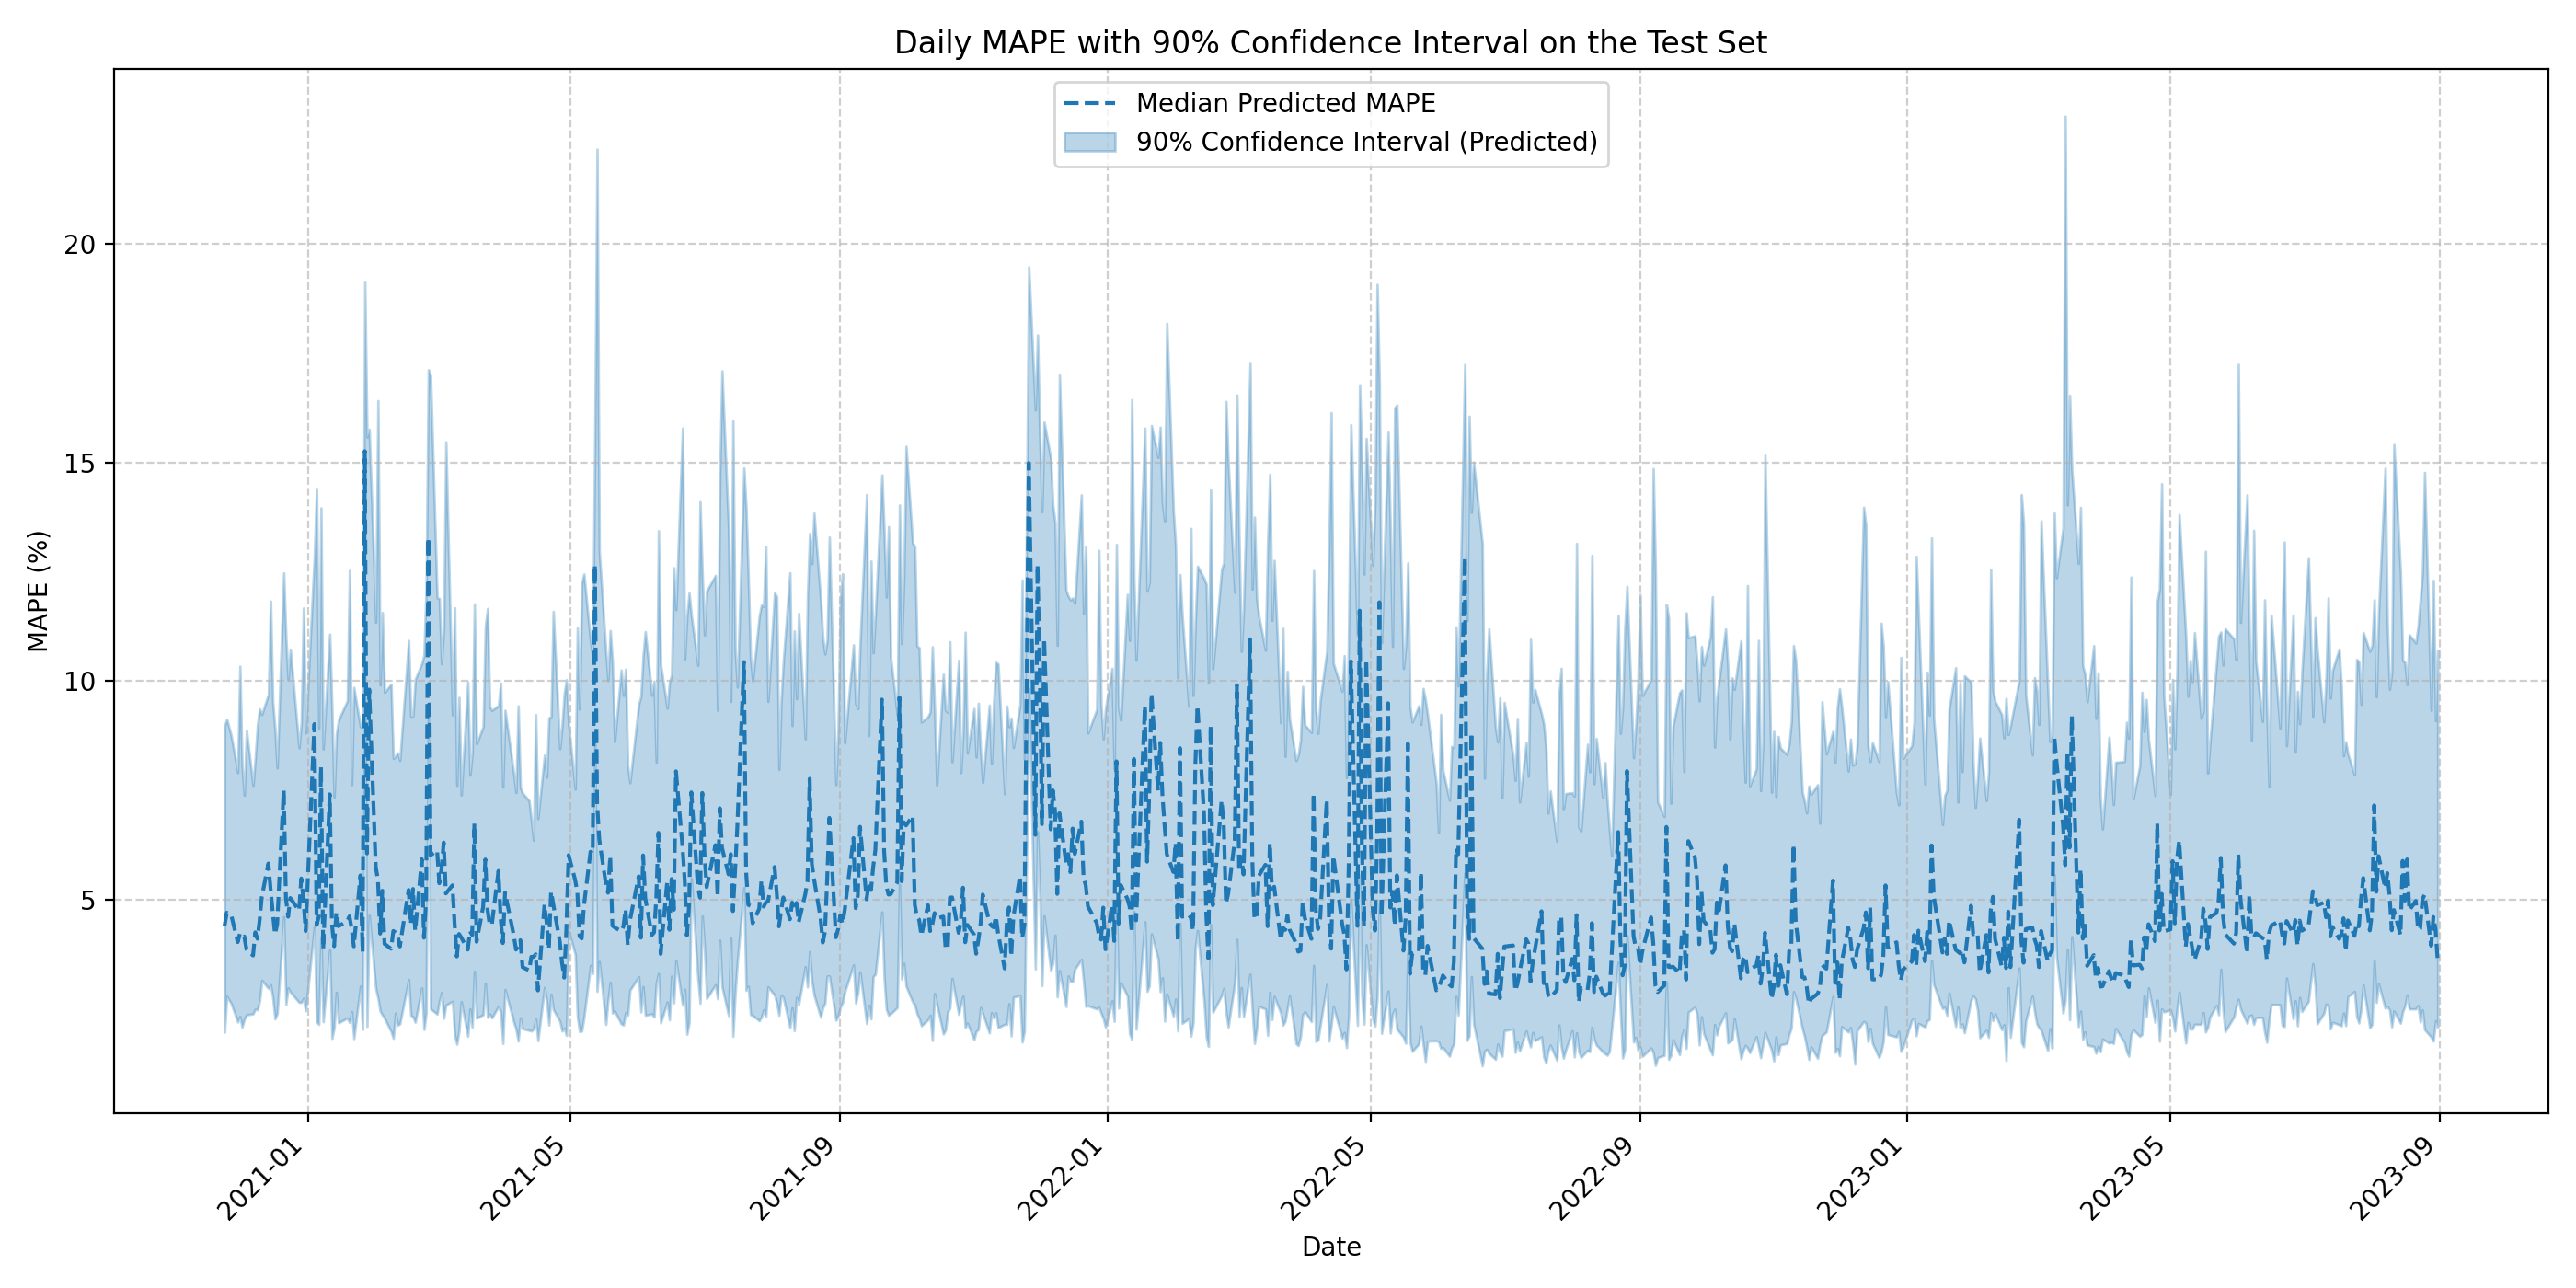
\includegraphics[width=0.9\textwidth]{fig/mape_timeseries_with_ci.png}
\end{figure}

\subsection{Financial Plausibility (Arbitrage Analysis)}
Beyond point-wise accuracy, a successful generative model for financial assets must produce outputs that are financially plausible and do not systematically violate fundamental no-arbitrage conditions. We evaluate this by calculating the total arbitrage penalty $\Phi$ (as defined in Equations \ref{eq:penalty_calendar}-\ref{eq:penalty_butterfly}) for every generated surface in the test set. Figure \ref{fig:arbitrage_timeseries} plots the daily mean arbitrage penalty generated by our conditional diffusion model against the ground-truth data from the test set. The plot displays the model's mean penalty (averaged over 100 generated samples per day). This is compared directly to the arbitrage penalty of the real (smoothed) surface (black line).
\begin{figure}[h!]
    \centering
    \caption{Daily Arbitrage Penalty of the Diffusion Model on the Test Set. The mean penalty (solid line) from our model are compared to the ground-truth penalty (black line).}
    \label{fig:arbitrage_timeseries}
    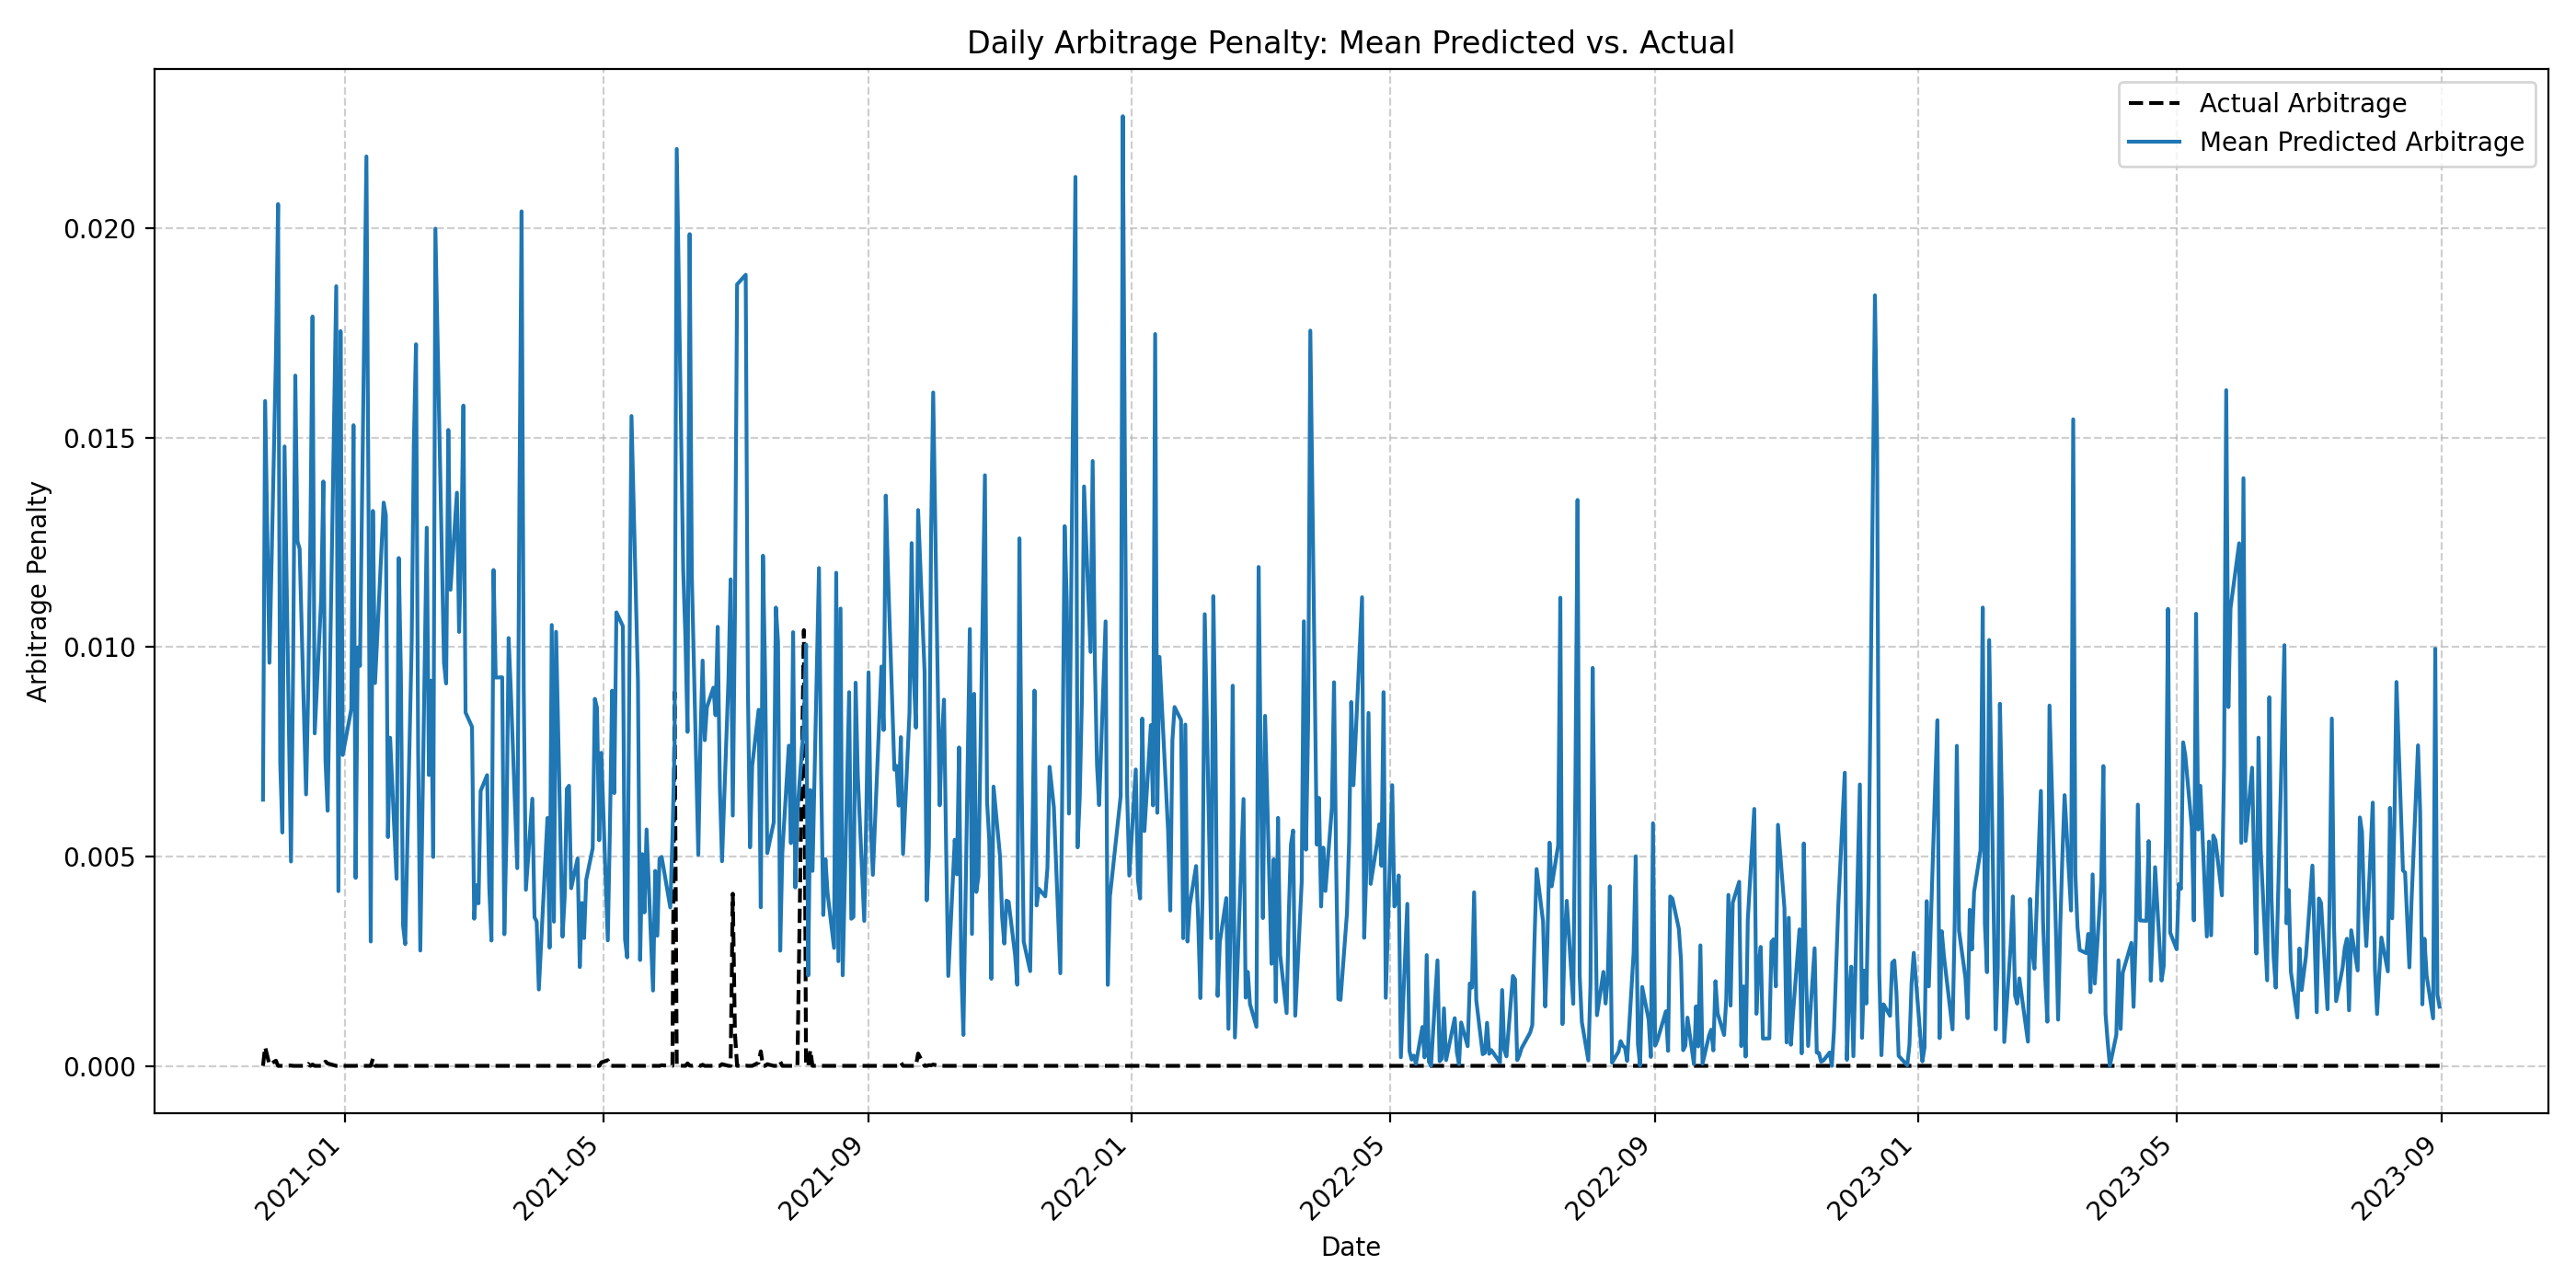
\includegraphics[width=0.9\textwidth]{fig/arbitrage_timeseries_mean.png}
\end{figure}

As shown in Figure \ref{fig:arbitrage_timeseries}, our model generates surfaces with relatively low arbitrage violations. The mean penalty consistently tracks the low-level penalty observed in the real test data, indicating that the model successfully captures the market's low-arbitrage characteristics. It is crucial to contextualize this result. Our training dataset (1996-2018) is composed of older market data. In these earlier periods, market microstructure was less advanced, and algorithmic trading was not as prevalent, leading to a higher incidence of arbitrage opportunities being recorded in the data. In contrast, our test set (2019-2023) reflects a modern, highly efficient market where high-frequency trading (HFT) and sophisticated arbitrage-seeking algorithms have made such opportunities far rarer.

This discrepancy presents a significant challenge: the models are trained on a distribution that contains a non-trivial amount of arbitrage. It is notoriously difficult for a data-driven generative model to learn to be ``cleaner'' than the data it is trained on. Therefore, the models inevitably learn to replicate some of these observed violations. Given this context, the ability of both the diffusion model and the GAN to generate surfaces with low arbitrage. It suggests that both models, despite being trained on imperfect data, are successfully capturing the underlying, dominant manifold structure of financially plausible surfaces and are not simply overfitting to the arbitrage-laden examples in the training set.

\subsection{Distributional and Structural Fidelity}
A robust generative model must replicate the mean of the data, the full statistical distribution, and underlying covariance structure at the same time. While the previous section confirmed the accuracy of the mean forecast, we now analyze whether our diffusion model successfully learns the complete, non-Gaussian distribution and the low-dimensional manifold structure of implied volatility surfaces. To assess distributional fidelity, we compare the higher-order statistical moments of the generated data against the real data. Volatility is well-known to be non-Gaussian, often exhibiting significant skewness and fat tails. A successful model must capture these features.

We analyze the marginal distributions for several key grid points by pooling all 100 generated samples for each of the 696 test days, creating a large sample distribution for both the model and the ground truth. Table \ref{tab:moments} compares the first four moments (Mean, Standard Deviation, Skewness, and Kurtosis) for five representative slices.
\begin{table}[h!]
    \centering
    \caption{Comparison of Statistical Moments for Key IV Slices (Test Set).}
    \label{tab:moments}
    \resizebox{\textwidth}{!}{%
    \begin{tabular}{lrrrrrrrrrr}
        \toprule
        Metric & \multicolumn{2}{c}{ATM 1-Day} & \multicolumn{2}{c}{ATM 1-Month} & \multicolumn{2}{c}{OTM 1-Week} & \multicolumn{2}{c}{OTM 3-Month} & \multicolumn{2}{c}{ITM 1-Week} \\
        \cmidrule(lr){2-3} \cmidrule(lr){4-5} \cmidrule(lr){6-7} \cmidrule(lr){8-9} \cmidrule(lr){10-11}
        & Real Data & Diffusion & Real Data & Diffusion & Real Data & Diffusion & Real Data & Diffusion & Real Data & Diffusion \\
        \midrule
        Mean & 0.1884 & 0.1868 & 0.1891 & 0.1876 & 0.1616 & 0.1622 & 0.1546 & 0.1548 & 0.3960 & 0.3914 \\
        Std Dev & 0.0448 & 0.0441 & 0.0439 & 0.0431 & 0.0230 & 0.0272 & 0.0221 & 0.0241 & 0.0371 & 0.0385 \\
        Skewness & 0.5487 & 0.6993 & 0.5339 & 0.6651 & 0.6318 & 0.7804 & 0.6201 & 0.6723 & 0.6887 & 0.7034 \\
        Kurtosis (Fisher) & -0.5404 & 0.1520 & -0.5562 & 0.0679 & 0.2771 & 1.0518 & 0.1709 & 0.4273 & 0.0930 & 0.6775 \\
        \bottomrule
    \end{tabular}
    }

    \caption*{Comparison of the first four statistical moments between the real data distribution and the pooled distribution of all generated samples from the diffusion model over the entire test set. Kurtosis is reported as Fisher's kurtosis (normal=0).}
\end{table}

\paragraph{Analysis of Distributional Moments.}
The results in Table \ref{tab:moments} provide several crucial insights. The first two moments (Mean and Std Dev) are very closely matched, confirming the point-wise accuracy observed in the previous subsection. Furthermore, the model correctly captures the positive skewness present in all the real data slices, a key non-Gaussian feature.

The most notable discrepancy, however, appears in the kurtosis. The real data consistently exhibits smaller kurtosis, indicating a distribution with thinner tails, more stable central peak. This is visually confirmed in Figure \ref{fig:histograms}, where the blue ``Real Data'' histograms appear wider and more rectangular. In contrast, our diffusion model generates data with a larger kurtosis. This indicates the model is producing fatter tails and a spikier central peak than the ground truth. This is also clearly visible in Figure \ref{fig:histograms}, where the orange ``Diffusion Model'' distribution is more sharply peaked and has more mass in the extreme tails. This implies that the model, while accurate on average, tends to overestimate the frequency of extreme volatility events. For a risk-management application, this could be interpreted as a conservative bias, as the model generates more stress scenarios than are present in the smoothed historical data. Our model is overestimating the tail risks than the actual data.

\begin{figure}[h!]
    \centering
    \caption{Distributional Comparison for Key IV Slices.}
    \label{fig:histograms}
    % --- FIRST ROW ---
    \begin{subfigure}[b]{0.49\textwidth}
        \centering
        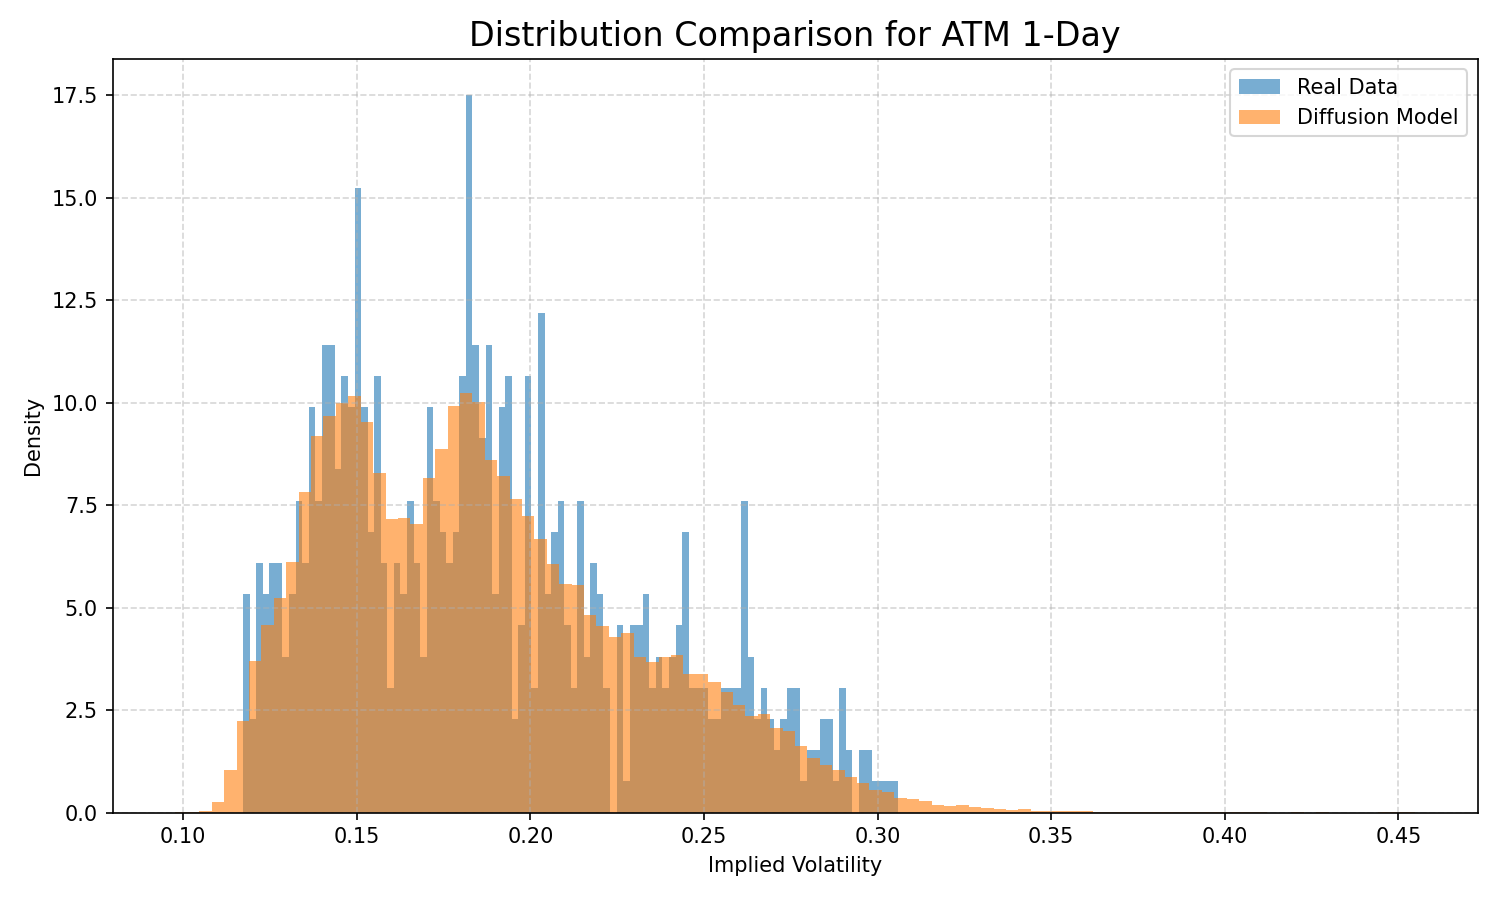
\includegraphics[width=\textwidth]{fig/Dist_ATM_1-Day_histogram.png}
        \caption{ATM 1-Day distribution histogram plot of real data and generated data.}
    \end{subfigure}
    \hfill
    \begin{subfigure}[b]{0.49\textwidth}
        \centering
        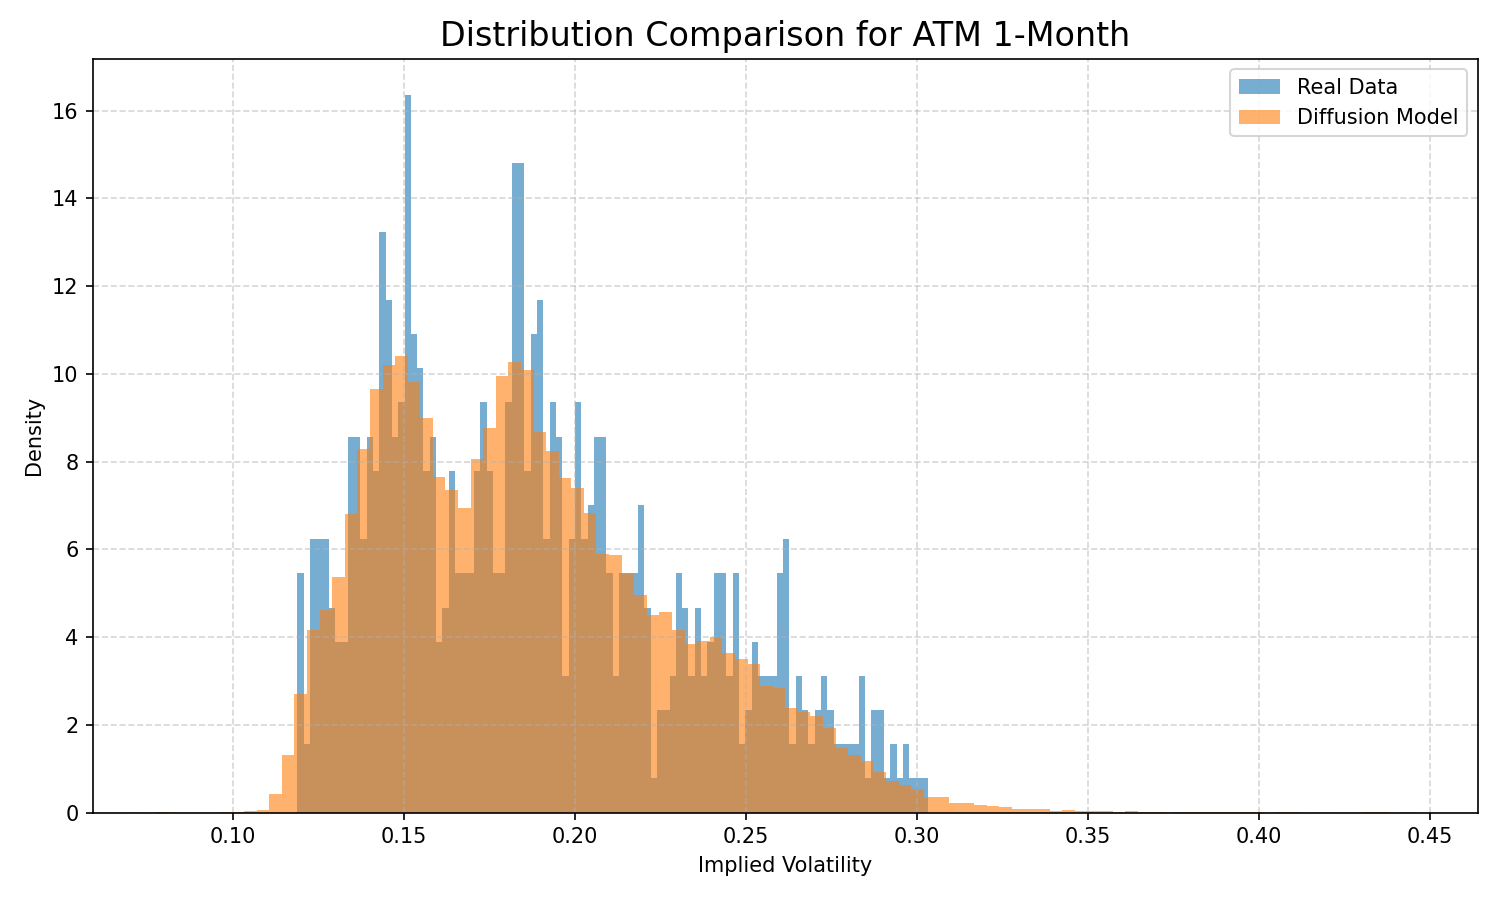
\includegraphics[width=\textwidth]{fig/Dist_ATM_1-Month_histogram.png}
        \caption{ATM 1-Month distribution histogram plot of real data and generated data.}
    \end{subfigure}

    \vspace{0.5cm} 

    % --- SECOND ROW ---
    \begin{subfigure}[b]{0.49\textwidth}
        \centering
        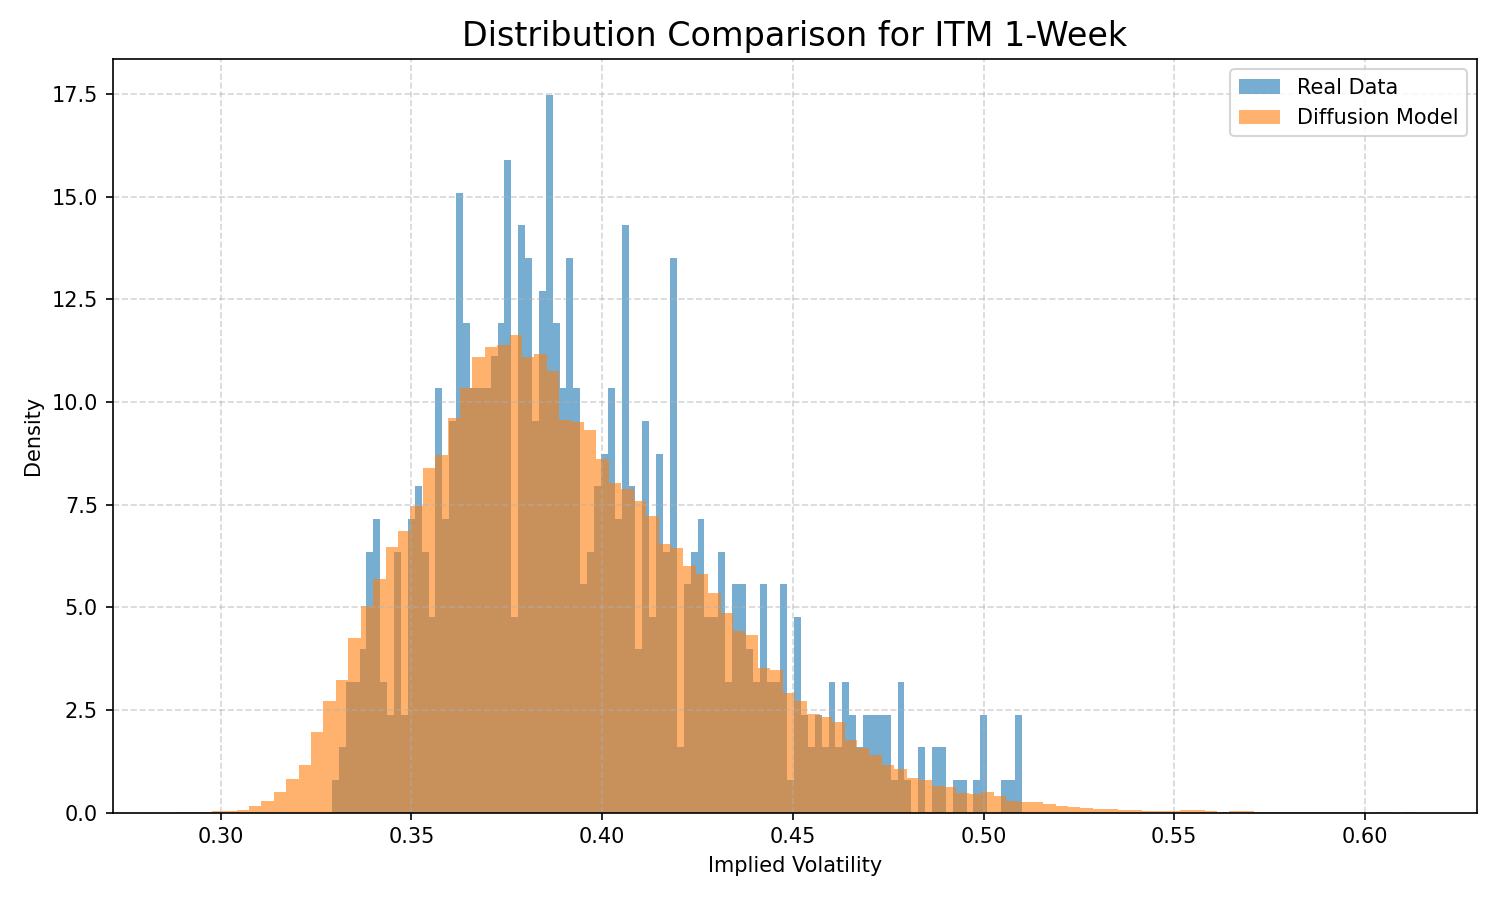
\includegraphics[width=\textwidth]{fig/Dist_ITM_1-Week_histogram.png}
        \caption{ITM 1-Week distribution histogram plot of real data and generated data.}
    \end{subfigure}
    \hfill
    \begin{subfigure}[b]{0.49\textwidth}
        \centering
        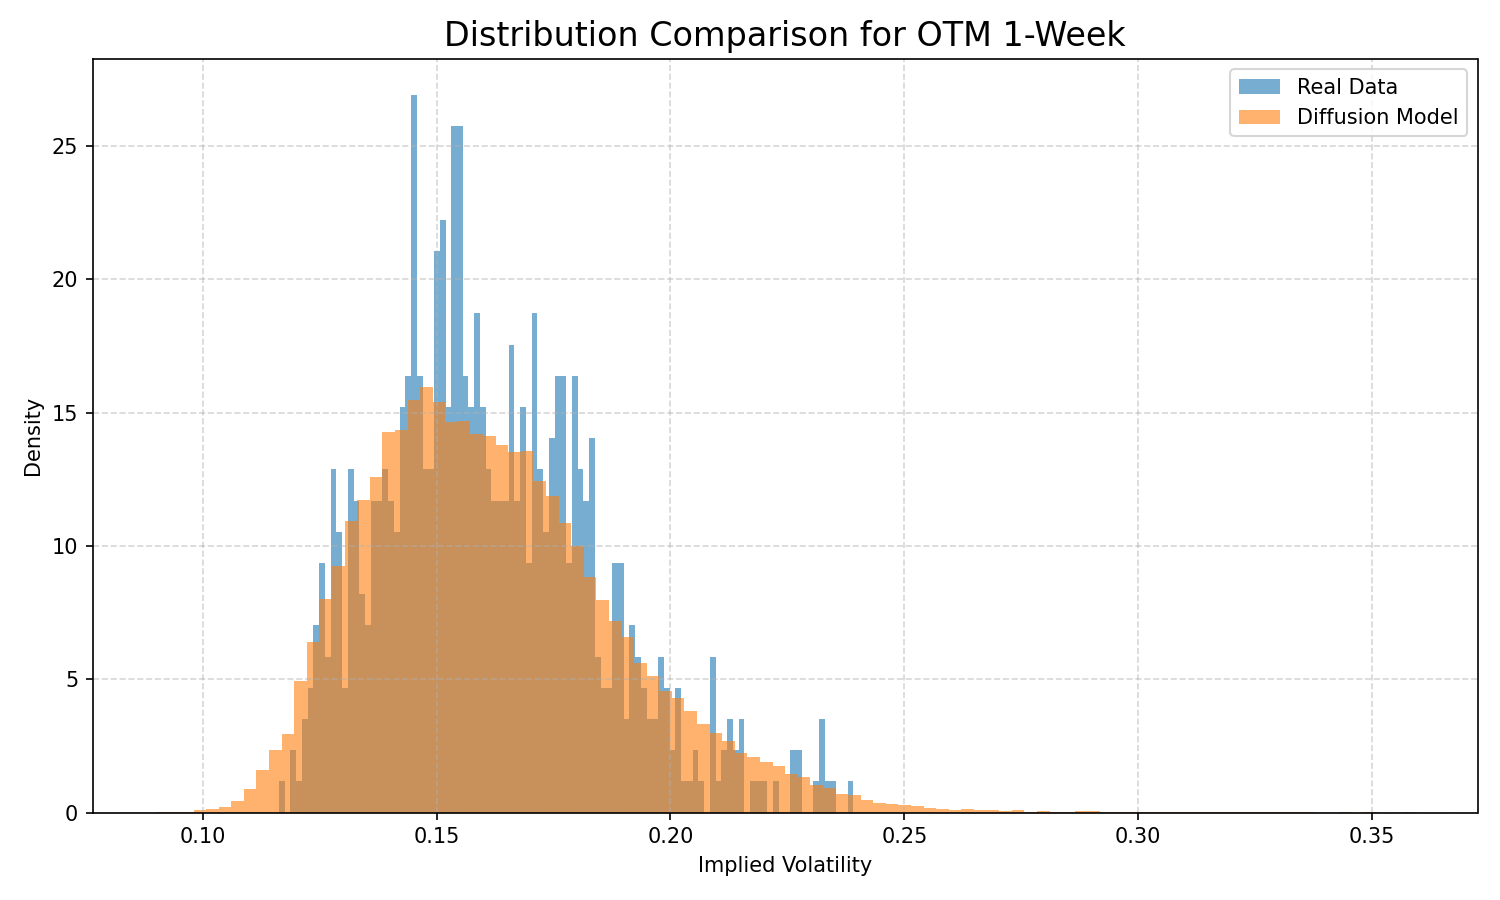
\includegraphics[width=\textwidth]{fig/Dist_OTM_1-Week_histogram.png}
        \caption{OTM 1-Week distribution histogram plot of real data and generated data.}
    \end{subfigure}

\end{figure}

\section{Conclusion}
\label{sec:conclusion}

In this paper, we introduced a conditional Denoising Diffusion Probabilistic Model (DDPM) for the one-day-ahead forecasting of implied volatility surfaces. We demonstrated that the stable training of diffusion models, combined with conditioning variables, provides a powerful and improved alternative to existing generative models like GANs.

We incorporates an explicit arbitrage penalty into the loss function that is dynamically weighted by the Signal-to-Noise Ratio (SNR). This approach successfully balances the financial plausibility, guiding the model towards the arbitrage-free manifold without destabilizing the training process given that the training data samples are not arbitrage-free. The empirical results confirmed the success of this method. Our model not only achieved a lower Overall MAPE than the VolGAN benchmark but, more critically, produced well-calibrated and statistically reliable 90\% confidence intervals.

Furthermore, we provided a formal convergence guarantee for this penalized loss, proving that the bias introduced by the penalty is bounded ($O(\lambda^2)$) and controllable. This result places our domain-specific loss function on a firm theoretical foundation, ensuring that the model's convergence properties are understood.

For future research, our model's uncertainty estimates for OTM options were shown to be overly conservative (CI breach rate $\approx$ 1\%). This could explore alternative loss-weighting schemes to improve calibration across the entire surface. Also, while our SNR-weighted penalty significantly reduces arbitrage, it remains a 'soft' constraint. Exploring methods to enforce arbitrage-free conditions as a 'hard' constraint, perhaps through a re-parameterization of the U-Net's output, would be a valuable extension.

\bibliographystyle{plainnat}
\bibliography{references}

\appendix
\section{Full Performance Metrics for All Trained Models}
\label{sec:appendix_full_table}

\begin{table}[h!]
\centering
\caption{Full comparison of performance metrics for all 9 trained VolGAN models and the proposed Diffusion model. VolGAN 5 was selected as the benchmark for comparison in the main text due to having the lowest Overall MAPE.}
\label{tab:full_performance_metrics}
\resizebox{\textwidth}{!}{%
\begin{tabular}{l rrrrrrrrrrrrr}
\toprule
% --- Hierarchical Column Headers ---
& \multicolumn{4}{c}{ATM} & \multicolumn{4}{c}{OTM} & \multicolumn{4}{c}{ITM} & \\
\cmidrule(lr){2-5} \cmidrule(lr){6-9} \cmidrule(lr){10-13}
% --- Sub-Headers ---
Metric & 1-Day & 1-Week & 1-Month & 3-Month & 1-Day & 1-Week & 1-Month & 3-Month & 1-Day & 1-Week & 1-Month & 3-Month & Overall \\
\midrule

% --- VolGAN 1 Data ---
\multicolumn{14}{l}{\textbf{VolGAN 1}} \\
MAPE (\%) & 7.0001 & 6.9535 & 6.5684 & 5.8614 & 9.4079 & 9.7788 & 8.6473 & 6.7865 & 4.9322 & 4.8257 & 4.2571 & 3.6685 & 6.6667 \\
Std. of APE (\%) & 4.2401 & 4.2771 & 4.1018 & 3.6491 & 5.8378 & 5.9709 & 5.3908 & 4.4841 & 3.0913 & 3.0571 & 2.7487 & 2.2577 &  \\
Mean CI Width & 0.0190 & 0.0192 & 0.0177 & 0.0183 & 0.0526 & 0.0504 & 0.0489 & 0.0355 & 0.0272 & 0.0225 & 0.0191 & 0.0100 &  \\
Std. CI Width & 0.0094 & 0.0092 & 0.0083 & 0.0058 & 0.0119 & 0.0108 & 0.0104 & 0.0076 & 0.0069 & 0.0055 & 0.0042 & 0.0019 &  \\
CI Breach \% & 87.2126 & 88.0747 & 88.5057 & 88.0747 & 48.2758 & 52.8735 & 48.7068 & 52.1551 & 85.1963 & 88.0747 & 89.6551 & 94.6839 &  \\
\addlinespace

% --- VolGAN 2 Data ---
\multicolumn{14}{l}{\textbf{VolGAN 2}} \\
MAPE (\%) & 4.2452 & 4.2468 & 4.1351 & 3.8260 & 4.3516 & 4.3417 & 4.1015 & 3.4180 & 2.5534 & 2.5314 & 2.4761 & 2.2700 & 3.1977 \\
Std. of APE (\%) & 4.2435 & 4.3466 & 4.1902 & 3.8217 & 4.1809 & 4.0501 & 4.1015 & 3.4180 & 2.4646 & 2.4578 & 2.3910 & 2.1277 &  \\
Mean CI Width & 0.0063 & 0.0063 & 0.0061 & 0.0057 & 0.0071 & 0.0070 & 0.0067 & 0.0059 & 0.0042 & 0.0041 & 0.0041 & 0.0039 &  \\
CI Breach \% & 32.4712 & 34.6537 & 33.7638 & 39.3090 & 41.5229 & 0.1437 & 0.5747 & 0.1437 & 35.6323 & 53.4482 & 66.2011 & 66.2011 &  \\
\addlinespace

% --- VolGAN 3 Data ---
\multicolumn{14}{l}{\textbf{VolGAN 3}} \\
MAPE (\%) & 4.9158 & 4.8870 & 4.7380 & 4.3006 & 5.0614 & 5.0153 & 4.7212 & 4.0155 & 3.5417 & 3.5375 & 3.0911 & 2.7011 & 4.3185 \\
Std. of APE (\%) & 4.1693 & 4.2790 & 4.1503 & 3.6596 & 5.4080 & 5.4496 & 5.0528 & 4.1803 & 2.8596 & 2.8687 & 2.7667 & 2.5827 &  \\
Mean CI Width & 0.0033 & 0.0033 & 0.0032 & 0.0030 & 0.0040 & 0.0040 & 0.0038 & 0.0033 & 0.0031 & 0.0030 & 0.0028 & 0.0025 &  \\
Std. CI Width & 0.0013 & 0.0013 & 0.0012 & 0.0011 & 0.0023 & 0.0023 & 0.0022 & 0.0017 & 0.0016 & 0.0015 & 0.0013 & 0.0011 &  \\
CI Breach \% & 71.2627 & 72.7011 & 74.2844 & 75.5747 & 92.9195 & 95.1150 & 95.1150 & 94.6839 & 82.3276 & 84.5229 & 94.4000 & 97.2701 &  \\
\addlinespace

% --- VolGAN 4 Data ---
\multicolumn{14}{l}{\textbf{VolGAN 4}} \\
MAPE (\%) & 4.9835 & 5.0119 & 4.7963 & 4.2089 & 5.3025 & 5.2542 & 4.8604 & 3.8761 & 3.2672 & 3.1011 & 2.7571 & 2.5994 & 4.2181 \\
Std. of APE (\%) & 4.2251 & 4.3025 & 4.1102 & 3.5221 & 5.2530 & 5.1780 & 4.6738 & 3.7088 & 2.7575 & 2.6288 & 2.3359 & 2.2215 &  \\
Mean CI Width & 0.0101 & 0.0101 & 0.0094 & 0.0087 & 0.0221 & 0.0210 & 0.0194 & 0.0146 & 0.0118 & 0.0101 & 0.0085 & 0.0059 &  \\
Std. CI Width & 0.0058 & 0.0057 & 0.0051 & 0.0039 & 0.0068 & 0.0064 & 0.0061 & 0.0045 & 0.0037 & 0.0031 & 0.0025 & 0.0015 &  \\
CI Breach \% & 62.0689 & 60.0574 & 59.1954 & 56.9080 & 46.8390 & 52.0114 & 41.2528 & 42.8160 & 53.4482 & 52.3005 & 53.0172 & 58.1609 &  \\
\addlinespace

% --- VolGAN 5 Data ---
\multicolumn{14}{l}{\textbf{VolGAN 5}} \\
MAPE (\%) & 4.8882 & 4.8595 & 4.6231 & 4.2498 & 5.5066 & 5.7265 & 5.0659 & 4.0762 & 2.9814 & 2.9420 & 2.6978 & 2.3652 & 3.7304 \\
Std. of APE (\%) & 4.0258 & 4.0304 & 3.9043 & 3.5292 & 4.8518 & 4.9798 & 4.3324 & 3.5471 & 2.4231 & 2.4151 & 2.2283 & 1.8661 &  \\
Mean CI Width & 0.0158 & 0.0159 & 0.0146 & 0.0151 & 0.0726 & 0.0679 & 0.0654 & 0.0474 & 0.0347 & 0.0292 & 0.0248 & 0.0128 &  \\
Std. CI Width & 0.0073 & 0.0072 & 0.0064 & 0.0047 & 0.0172 & 0.0149 & 0.0141 & 0.0099 & 0.0091 & 0.0075 & 0.0055 & 0.0023 &  \\
CI Breach \% & 44.8276 & 43.8218 & 45.6897 & 40.5172 & 1.5805 & 2.5862 & 1.0057 & 1.0057 & 31.4655 & 35.0575 & 36.7816 & 57.1839 &  \\
\addlinespace

% --- VolGAN 6 Data ---
\multicolumn{14}{l}{\textbf{VolGAN 6}} \\
MAPE (\%) & 4.5919 & 4.5842 & 4.4827 & 3.9911 & 4.9067 & 4.9871 & 4.1293 & 2.9027 & 2.9071 & 2.8081 & 2.5404 & 2.3304 & 3.5186 \\
Std. of APE (\%) & 4.0725 & 4.0620 & 3.9161 & 3.4862 & 4.4363 & 4.4077 & 3.8340 & 2.7309 & 2.4116 & 2.3661 & 2.1936 & 1.9480 &  \\
Mean CI Width & 0.0012 & 0.0012 & 0.0012 & 0.0011 & 0.0052 & 0.0048 & 0.0045 & 0.0031 & 0.0016 & 0.0015 & 0.0013 & 0.0009 &  \\
Std. CI Width & 0.0003 & 0.0003 & 0.0003 & 0.0003 & 0.0016 & 0.0014 & 0.0013 & 0.0008 & 0.0004 & 0.0004 & 0.0003 & 0.0002 &  \\
CI Breach \% & 97.2701 & 96.5528 & 97.5574 & 97.8448 & 98.1321 & 100 & 98.1321 & 100 & 94.1150 & 94.8275 & 94.2586 & 95.6896 &  \\
\addlinespace

% --- VolGAN 7 Data ---
\multicolumn{14}{l}{\textbf{VolGAN 7}} \\
MAPE (\%) & 5.2086 & 5.4404 & 5.0933 & 3.5758 & 10.2165 & 10.4572 & 5.3888 & 9.4522 & 2.7654 & 2.4677 & 2.2042 & 2.0596 & 5.1002 \\
Std. of APE (\%) & 4.1430 & 4.1090 & 3.7958 & 3.0917 & 6.2425 & 5.6217 & 4.3046 & 4.5954 & 2.1034 & 1.9688 & 1.8387 & 1.9649 &  \\
Mean CI Width & 0.0023 & 0.0023 & 0.0021 & 0.0017 & 0.0066 & 0.0059 & 0.0052 & 0.0040 & 0.0020 & 0.0017 & 0.0014 & 0.0009 &  \\
Std. CI Width & 0.0005 & 0.0005 & 0.0004 & 0.0003 & 0.0022 & 0.0019 & 0.0017 & 0.0010 & 0.0004 & 0.0003 & 0.0003 & 0.0002 &  \\
CI Breach \% & 96.9827 & 95.8390 & 95.5517 & 95.6954 & 95.6954 & 96.2643 & 98.8505 & 98.4195 & 91.0919 & 93.4023 & 96.1206 & 96.8390 &  \\
\addlinespace

% --- VolGAN 8 Data ---
\multicolumn{14}{l}{\textbf{VolGAN 8}} \\
MAPE (\%) & 9.2638 & 9.5120 & 9.5430 & 8.5866 & 5.5670 & 5.5821 & 5.1200 & 6.1042 & 4.9452 & 4.8576 & 4.8285 & 7.4301 & 6.7358 \\
Std. of APE (\%) & 4.9066 & 4.9712 & 4.9123 & 4.6773 & 5.1664 & 5.1768 & 4.7981 & 4.9984 & 3.5358 & 3.4839 & 3.5117 & 4.6300 &  \\
Mean CI Width & 0.0019 & 0.0019 & 0.0018 & 0.0017 & 0.0022 & 0.0022 & 0.0020 & 0.0019 & 0.0017 & 0.0016 & 0.0016 & 0.0022 &  \\
Std. CI Width & 0.0015 & 0.0015 & 0.0015 & 0.0013 & 0.0019 & 0.0019 & 0.0017 & 0.0013 & 0.0012 & 0.0011 & 0.0012 & 0.0015 &  \\
CI Breach \% & 93.5468 & 95.6954 & 95.4080 & 89.7988 & 79.5977 & 83.1609 & 83.1609 & 73.1321 & 83.5919 & 90.6609 & 98.9942 & 99.4252 &  \\
\addlinespace

% --- VolGAN 9 Data ---
\multicolumn{14}{l}{\textbf{VolGAN 9}} \\
MAPE (\%) & 7.0862 & 6.8310 & 6.2417 & 5.2863 & 8.0195 & 7.9536 & 7.0454 & 5.4578 & 5.1714 & 4.7146 & 3.9676 & 3.6654 & 6.0554 \\
Std. of APE (\%) & 4.7099 & 4.5428 & 4.1795 & 3.5511 & 6.0827 & 5.8643 & 5.2443 & 4.1952 & 3.8229 & 3.4960 & 2.9248 & 2.6517 &  \\
Mean CI Width & 0.0069 & 0.0067 & 0.0061 & 0.0053 & 0.0128 & 0.0121 & 0.0110 & 0.0082 & 0.0093 & 0.0079 & 0.0064 & 0.0044 &  \\
Std. CI Width & 0.0022 & 0.0021 & 0.0019 & 0.0015 & 0.0043 & 0.0039 & 0.0035 & 0.0025 & 0.0029 & 0.0023 & 0.0018 & 0.0011 &  \\
CI Breach \% & 90.0862 & 90.0862 & 91.0919 & 92.2356 & 94.2586 & 95.1150 & 95.1150 & 96.1206 & 90.8045 & 93.1149 & 95.8390 & 100 &  \\
\addlinespace

% --- Diffusion Data ---
\multicolumn{14}{l}{\textbf{Diffusion}} \\
MAPE (\%) & 4.6907 & 4.6884 & 4.5146 & 4.0202 & 3.5264 & 3.4573 & 3.1542 & 2.4555 & 2.5129 & 2.4992 & 2.4184 & 2.2024 & 3.0026 \\
Std. of APE (\%) & 4.0338 & 4.0091 & 3.8795 & 3.4909 & 2.6588 & 2.5785 & 2.3190 & 1.8739 & 2.3984 & 2.3844 & 2.2909 & 2.0393 &  \\
Mean CI Width & 0.0372 & 0.0369 & 0.0357 & 0.0327 & 0.0468 & 0.0457 & 0.0412 & 0.0311 & 0.0472 & 0.0463 & 0.0438 & 0.0384 &  \\
Std. CI Width & 0.0160 & 0.0159 & 0.0152 & 0.0134 & 0.0098 & 0.0095 & 0.0082 & 0.0057 & 0.0139 & 0.0137 & 0.0132 & 0.0124 & \\
CI Breach \% & 10.9195 & 10.4885 & 11.0632 & 10.0575 & 0.5747 & 0.7184 & 0.5747 & 1.0057 & 7.9023 & 7.9023 & 8.4770 & 7.9023 &  \\
\bottomrule
\end{tabular}
}
\end{table}

\end{document}
